% This is samplepaper.tex, a sample chapter demonstrating the
% LLNCS macro package for Springer Computer Science proceedings;
% Version 2.21 of 2022/01/12
%
\documentclass[runningheads]{llncs}
%\documentclass[draft]{llncs}
%
\usepackage[T1]{fontenc}
% T1 fonts will be used to generate the final print and online PDFs,
% so please use T1 fonts in your manuscript whenever possible.
% Other font encondings may result in incorrect characters.
%
\usepackage{graphicx}
\usepackage{hyperref}
% Used for displaying a sample figure. If possible, figure files should
% be included in EPS format.
%
% If you use the hyperref package, please uncomment the following two lines
% to display URLs in blue roman font according to Springer's eBook style:
\usepackage{color}
\renewcommand\UrlFont{\color{blue}\rmfamily}
\urlstyle{rm}

\usepackage{amsmath}
\usepackage{amssymb}
\usepackage{tikz}
\usepackage{wrapfig}
\usepackage{environ}
\usepackage{bbm}

\usepackage{changes}
\usepackage{algorithm}
\usepackage[noend]{algpseudocode}
\usepackage{varwidth}
\usepackage{mathtools}
\usepackage{pgfplots}
\usepackage[dvipsnames]{xcolor}
\usepackage[utf8]{inputenc}
\pgfplotsset{compat=1.18}
\usetikzlibrary {spy,arrows.meta,decorations.shapes}
\setauthormarkup{}
\definechangesauthor[name=jo, color=blue]{JO}
\definechangesauthor[name=rom, color=teal]{ROM}

% set of real numbers
\newcommand{\R}{\ensuremath{\mathbb{R}}}
% set of integer numbers
\newcommand{\Z}{\ensuremath{\mathbb{Z}}}
% cell complex build on the lattice \Z^d
\let\C\relax \DeclareMathOperator{\C}{\ensuremath{\mathcal{C}^d}} % modified because of incompatiblity with hyperref package
% cardinality of a set
\newcommand{\Card}[1]{\ensuremath{\#\left( #1 \right)}}
% Interior of a closed set.
\newcommand{\Int}[1]{\ensuremath{\mathrm{Int}\left( #1 \right)}}
% Some vectors and matrices
\newcommand{\vx}[0]{\ensuremath{\mathbf{x}}}
\newcommand{\vy}[0]{\ensuremath{\mathbf{y}}}
\newcommand{\vz}[0]{\ensuremath{\mathbf{z}}}
\newcommand{\vb}[0]{\ensuremath{\mathbf{b}}}
\newcommand{\vA}[0]{\ensuremath{\mathbf{A}}}
\newcommand{\va}[0]{\ensuremath{\mathbf{a}}}
\newcommand{\vc}[0]{\ensuremath{\mathbf{c}}}
\newcommand{\ve}[0]{\ensuremath{\mathbf{e}}}
\newcommand{\vm}[0]{\ensuremath{\mathbf{m}}}
\newcommand{\vn}[0]{\ensuremath{\mathbf{n}}}
\newcommand{\vu}[0]{\ensuremath{\mathbf{u}}}
\newcommand{\vv}[0]{\ensuremath{\mathbf{v}}}
\newcommand{\vw}[0]{\ensuremath{\mathbf{w}}}
\newcommand{\vp}[0]{\ensuremath{\mathbf{p}}}
\newcommand{\vq}[0]{\ensuremath{\mathbf{q}}}
\newcommand{\vr}[0]{\ensuremath{\mathbf{r}}}
\newcommand{\vs}[0]{\ensuremath{\mathbf{s}}}
\newcommand{\vt}[0]{\ensuremath{\mathbf{t}}}
% Convex hull
\newcommand{\Conv}[1]{\mathrm{CvxH}\left( #1 \right)}

% References
\newcommand{\Equ}[1]{(\ref{#1})}
\newcommand{\RefFigure}[1]{Figure~\ref{#1}}
\newcommand{\RefLemma}[1]{Lemma~\ref{#1}}
\newcommand{\RefLemmas}[2]{Lemmas~\ref{#1} and~\ref{#2}}
\newcommand{\RefTheorem}[1]{Theorem~\ref{#1}}
\newcommand{\RefCorollary}[1]{Corollary~\ref{#1}}
\newcommand{\RefAlgorithm}[1]{Algorithm~\ref{#1}}
\newcommand{\RefSection}[1]{Section~\ref{#1}}
\newcommand{\Refline}[1]{line~\ref{#1}}
\newcommand{\RefLine}[1]{Line~\ref{#1}}

% Star, closure, boundary of a complex
\newcommand{\Bd}[1]{\ensuremath{\mathrm{Bd}\left(#1\right)}}
\newcommand{\Star}[1]{\ensuremath{\mathrm{Star}\left(#1\right)}}
\newcommand{\Starop}[0]{\ensuremath{\mathrm{Star}}}
\newcommand{\Cl}[1]{\ensuremath{\mathrm{Cl}\left(#1\right)}}
% Closed interior
\newcommand{\CI}[1]{\ensuremath{\mathrm{ClInt}\left(#1\right)}}
% Body of a complex
\newcommand{\Body}[1]{\ensuremath{\left\|#1\right\|}}
% topological closure
\newcommand{\TCl}[1]{\ensuremath{\overline{#1}}}
% topological interior
\newcommand{\TInt}[1]{\ensuremath{\mathring{#1}}}
% topological boundary
\newcommand{\TBd}[1]{\ensuremath{\partial{#1}}}
% <=
\newcommand{\Le}{\ensuremath{\leqslant}}
% >=
\newcommand{\Ge}{\ensuremath{\geqslant}}


% Euclidean distance
\newcommand{\EDist}[0]{\ensuremath{\mathrm{d}_\mathbf{E}}}
% Hausdorff distance
\newcommand{\HDist}[0]{\ensuremath{\mathrm{d}_H}}
% Normal cone to S at p
\newcommand{\NC}[2]{\ensuremath{\mathrm{N}_{#1}(#2)}}

% l2 norm
\newcommand{\ltwo}[0]{\ensuremath{\ell_2}}
\newcommand{\loo}[0]{\ensuremath{\ell_\infty}}

% Reach
\newcommand{\Reach}[1]{\ensuremath{\mathrm{reach}(#1)}}
% Volume
\newcommand{\Vol}[1]{\ensuremath{\mathrm{Vol}\left(#1\right)}}
\newcommand{\Vold}[2]{\ensuremath{\mathrm{Vol}^{#1}\left(#2\right)}}
% Digitization
\newcommand{\Dig}[2]{\ensuremath{\mathrm{D}_{#1}\left(#2\right)}}
% Counting lattice points
\newcommand{\Lat}[1]{\ensuremath{\mathcal{L}_{#1}}}
\newcommand{\LatC}[2]{\ensuremath{\Lat{#1}(#2)}}


%
\begin{document}
%
    \title{Fast and exact visibility on digitized shapes and application to saliency-aware normal estimation}
%
    \titlerunning{Fast and exact visibility on digitized shapes}
% If the paper title is too long for the running head, you can set
% an abbreviated paper title here
%
    \author{Romain Negro\inst{1}\orcidID{0000-XXXX-YYYY-ZZZZ} \and
    Jacques-Olivier Lachaud\inst{1}\orcidID{0000-0003-4236-2133}}
%
    \authorrunning{R. Negro and J.-O. Lachaud}
% First names are abbreviated in the running head.
% If there are more than two authors, 'et al.' is used.
%
    \institute{Universit\'e Savoie Mont Blanc, CNRS, LAMA, F-73000 Chambéry, France\\
    \email{\{romain.negro|jacques-olivier.lachaud\}@univ-smb.fr}}
%
    \maketitle              % typeset the header of the contribution
%
    \begin{abstract}
        Computing visibility on a geometric object requires heavy
        computations since it requires to identify pairs of points that
        are visible to each other, i.e.\ there is a straight segment
        joining them that stays in the close vicinity of the object
        boundary. We propose to exploit a specific representation of
        digital sets based on lists of integral intervals in order to
        compute efficiently the complete visibility graph between
        lattice points of the digital shape. As a quite direct
        application, we show then how we can use visibility to estimate
        the normal vector field of a digital shape in an accurate and
        convergent manner while staying aware of the salient and sharp features of
        the shape.

        \keywords{Visibility \and Geometric inference \and Digital normal estimation \and Digital geometry}
    \end{abstract}

%%%%%%%%%%%%%%%%%%%%%%%%%%%%%%%%%%%%%%%%%%%%%%%%%%%%%%%%%%%%%%%%%%%%%%


    \section{Introduction}
        Visibility is a fundamental concept in computational geometry and
    digital topology, with applications ranging from computer vision
    (occlusions), geometric modeling (feature detection,
    geodesics) to computer graphics (path tracing,
    shadowmap). Visibility within polygons in the plane has been
    extensively studied in the litterature~\cite{ghosh:2007-book} and
    is still studied in higher dimensional
    spaces~\cite{orourke:2017-book}. The general problem has a high
    complexity. For instance, the 3d visibility complex between $n$
    spheres and occluding spheres has a complexity
    $O(n^4)$~\cite{durand:2002-tog}. Exact 3d visibility between
    polygons and occluding polygons is often cast into 5d Plücker
    space~\cite{nirenstein:2002-ewr}, which nicely represents 3d lines
    and their respective positions. The computational cost remains
    high even with decomposition into coarse cells for speed up
    (several days of computation for 1M triangles at the time).

    To increase efficiency, several authors have cast the
    visibility problem into a digital space, generally $\Z^3$ or its
    decomposition into cubical cells. Visibility is simplified as
    whether there is a connected digital straight line
    joining a pair of cells without occluding cell(s)
    (e.g.\ Soille~\cite{soille:1994-prl} uses Bresenham
    segments). Coeurjolly \emph{et al.}~\cite{coeurjolly:2004-prl}
    use a non-symmetric visibility definition and preimage
    computations to speed up these
    algorithms. Chica~\cite{chica:2008-spm} uses a half-cell erosion
    of the complementary space and Bresenham lines to decide
    visibility.

    We propose an algorithm that solves the following visibility
    problem: given a digital set $X \subset \Z^d$, two points $p,q$ of
    $X$ are \emph{visible} whenever the Euclidean straight line
    segment $\lbrack p,q \rbrack$ is never at chessboard distance
    ($\infty$-distance) greater or equal to $1$ from $X$. It is
    equivalent to the \emph{cotangency} of $p$ and $q$ in $X$, as
    formalized in~\cite{lachaud:2021-dgmm,lachaud:2022-jmiv}, and can
    be viewed as an inclusion problem between sets of lattice points
    in this form. Indeed, cells surounding $X$ can be encoded as
    lattice points (Khalimsky coding), as well as the cells covering
    lattice directions. The originality of our method is to encode
    subsets of lattice points as sets of integer intervals and to
    reduce all the inclusion problems as intersections and
    translations of integer intervals. For a given lattice vector
    $\mathbf{t}$, we solve the visibility of every pair of points
    $(p,p+\mathbf{t})$ of $X$. Global visibility is achieved by
    testing all sought directions within a given range, and is
    parallelized straightforwardly.

    We focus on solving efficiently this problem because it is crucial
    in computing geometric normals along digital surfaces that are
    aware of salient features. Indeed, 2d discrete tangent estimators
    based on tangency or discrete line segments have proven to be both
    sensitive to sharp corners and multigrid convergent on the
    boundary of digitized smooth shapes~\cite{feschet:1999-dgci,lachaud:2007-ivc,nguyen:2011-pr}.
    Many ad hoc methods have been proposed for tangent plane or normal
    estimation on 3d digital surfaces
    (e.g. \cite{fourey:2009-cg,charrier:2011-iwcia,Cuel:2014-dgci,Lachaud:2017-lnm,mareche:2024-ispr}).
    If two of these methods~\cite{Cuel:2014-dgci,Lachaud:2017-lnm}
    have been shown to be multigrid convergent on digitization of
    shapes with smooth boundary, their formulation intrinsically
    smoothes features, e.g.\ in contrast with the method of
    Mar{ê}ch{é} \emph{et al.}~\cite{mareche:2024-ispr}, whose
    convergence is not established. We propose here a normal estimator
    defined as the most orthogonal vector to the cone of visibility at
    the point of interest. Visibility is high in smooth regions and
    the induced visibility vectors are good approximations of tangent
    vectors. On the contrary the visibility is blocked at sharp
    features, so the normal vector is not influenced by the
    geometry on the other side of the features. We demonstrate the
    superiority of this normal estimator for estimating curvatures
    along digital surfaces with sharp features.

    Note that our algorithm for computing visibility is in fact much
    more general. The same algorithm could be used to recognize if any
    pattern of lattice points is present on a shape. It is similar to
    an erosion algorithm where the structuring element is the chosen
    pattern, and could also be used for morphological operations~\cite{soille1999morphological}.
    The paper outline is as follows. In Section~2, we recall some
    definitions and present tangency of chords and its equivalence
    to visibility. Section~3 describes the specific data structure
    for encoding set of grid cells, and the main algorithm that
    exploits this encoding to compute visibility exactly. Section~4
    presents experimental results on visibility, its usage as a
    discrete normal estimator, and how it improves curvature estimates
    on digital surfaces. Finally, Section 5 concludes and gives some
    perspectives to this work.
    %% , notably other usages of this algorithm in the field.

%    \deleted[id=JO]{
%    Visibility is a fundamental concept in computational geometry and digital topology, with applications ranging from computer vision to geometric modeling and computer graphics.
%    In this work, we explore visibility through the lens of chord tangency, introducing a novel approach that builds on discrete geometric structures.
%    Our framework leverages the discrete setting of and cell complexes, providing a rigorous foundation for analyzing visibility properties in digital spaces.
%    }
%
%
%    \deleted[id=JO]{
%    We recall essential definitions from previous works, particularly the notions of cell complexes and the star operator as formalized in~\cite{lachaud:2021-dgmm} and~\cite{lachaud:2022-jmiv}.
%    The integer grid serves as our primary space of study, where geometric structures are discretized using cell complexes.
%    A cell complex is a decomposition of space into elementary units (vertices, edges, faces, and higher-dimensional counterparts) forming a combinatorial representation of geometric objects.
%    The star of a cell, as defined in these works, consists of all higher-dimensional cells that contain it, a crucial concept for analyzing local neighborhoods and connectivity.
%    }
%
%    \deleted[id=JO]{
%      Building on these foundations, our study focuses on visibility as determined by the tangency of chords in discrete geometry.
%    We define and analyze how visibility relationships emerge in this context and investigate their combinatorial and topological implications.
%    This approach provides a new perspective on discrete visibility, offering potential applications in digital imaging, surface reconstruction, and computational topology.
%    }
%
%    \deleted[id=JO]{
%      The remainder of this paper is structured as follows.
%    In Section 2, we formalize the concept of chord tangency and its role in visibility analysis.
%    Section 3 enters into the usage of integer intervals intersections to quickly scan the figure in order to recover this visibiltiy.
%    Section 4 presents our main results, using this visibility to compute normals using the CNC estimator~\cite{lachaud:2022-dcg}.
%    Finally, Section 5 concludes with some other applications of integer intervals intersections in the field.
%    }


%%%%%%%%%%%%%%%%%%%%%%%%%%%%%%%%%%%%%%%%%%%%%%%%%%%%%%%%%%%%%%%%%%%%%%


    \section{Visibility through tangency of chords}
        All the theory and algorithms presented in this section are
    defined and valid in arbitrary dimension $d$. They will however be
    illustrated in 2d for clarity, while experiments willl be
    performed on 3d digital shapes.  Let $\Z^d$ be the $d$-dimensional
    digital space.  Let $\mathcal{C}^d$ be the (cubical) cell complex
    induced by the lattice $\Z^d$ : its 0-cells are the points of
    $\Z^d$, its 1-cells are the open unit segments joining two 0-cells
    at distance 1, its 2-cells are the open unit squares, \ldots, and
    its $d$-cells are the $d$-dimensional open unit hypercubes with
    vertices in $\Z^d$.  We denote by $\mathcal{C}^d_k$ the set of its
    $k$-cells, for $0 \Le k \Le d$.  In the following, a cell always
    designates an element of $\mathcal{C}^d$, and the term subcomplex
    always indicates a subset of $\mathcal{C}^d$.

    The \emph{topological closure} of a cell $\tau$ is denoted by
    $\bar{\tau}$. The \emph{star} of a cell $\sigma$ is the subcomplex
    $\Star{\sigma}\coloneqq\{\tau \in \mathcal{C}, \sigma \subset \bar{\tau}
    \}$. It is naturally extended to any subcomplex $K$ by union,
    i.e. $\Star{K} \coloneqq \cup_{\sigma \in K} \Star{\sigma}$, and more
    generally to any subset $Y$ of $\R^d$ as $\Star{Y}\coloneqq\{ c \in \C,
    \bar{c} \cap Y \neq \emptyset \}$. The \emph{body} $\|K\|$ of $K$
    is its realization in $\R^d$, i.e. $\|K\|\coloneqq\cup_{c \in K} c$. One
    can check that $\Star{K}=\Star{\|K\|}$, so these definitions are
    sound.

    %% A cell $\sigma$ is a face of another cell $\tau$ whenever $\sigma$
    %% is a subset of the topological closure $\bar{\tau}$ of $\tau$,
    %% written $\sigma \preccurlyeq \tau$.  Given any subcomplex K of
    %% $\mathcal{C}^d$, the star $Star(K)$ of K is $\{\tau \in
    %% \mathcal{C}^d, s.t.\ \exists\sigma \in K,\sigma \preccurlyeq
    %% \tau\}$.
    \begin{definition}[Visibility]
      Let $Z \subset \Z^d$ be a digital set. Two digital points $p$
      and $q$ are \emph{visible in $Z$} if and only if the straight
      segment $[p, q]$ is included in $\Star{Z}$, i.e., $\Star{[p, q]}
      \subseteq \Star{Z}$.
    \end{definition}
    This definition corresponds to the concept of tangency presented
    in~\cite{lachaud:2022-jmiv}, limited to pairs of points. One can
    check that $p$ and $q$ must belong to $Z$ to be visible.
    Figure~\ref{fig:visibility-2d} illustrates what is considered
    visible or not on some examples.


    % Examples of visibility in 2D
    \begin{figure}[t]
      \centering
      \begin{tabular}{c@{~}|@{~}c@{~}|@{~}c@{~}|@{~}c}
  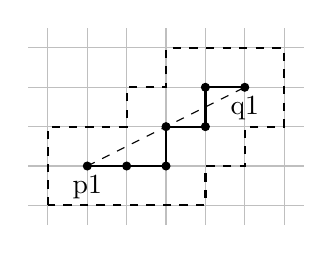
\begin{tikzpicture}
    \draw[step=0.5,lightgray,thin,xshift=-1cm,yshift=-1cm] (0.25,0.25) grid (3.75,2.75);
    \draw[dashed] (0,0) -- (2,1);
    \filldraw[black] (0,0) circle (0.05) node[anchor=north] {p1};
    \filldraw[black] (2,1) circle (0.05) node[anchor=north] {q1};
    \foreach \x/\y in {1/0,2/0,2/1,3/1,3/2} {
      \filldraw[black] (0.5*\x,0.5*\y) circle (0.05);
    }
    \draw [thick] (0,0) -- (0.5,0) -- (1,0) -- (1,0.5) -- (1.5,0.5) -- (1.5,1) -- (2,1);
    \draw[thick,dashed] (-0.5,-0.5) -- (-0.5,0.5) -- (0.5,0.5) -- (0.5,1) -- (1,1) -- (1,1.5) -- (2.5,1.5) -- (2.5,0.5) -- (2,0.5) -- (2,0) -- (1.5,0) -- (1.5,-0.5) -- (-0.5,-0.5);
  \end{tikzpicture} &
  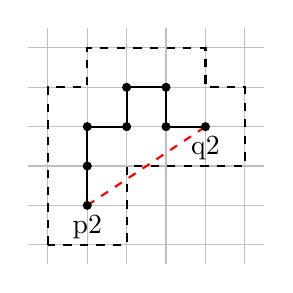
\begin{tikzpicture}
    \draw[step=0.5,lightgray,thin,xshift=-1cm,yshift=-1cm] (0.25,0.25) grid (3.25,3.25);
    \draw[red,dashed,thick] (0,0) -- (1.5,1);
    \filldraw[black] (0,0) circle (0.05) node[anchor=north] {p2};
    \filldraw[black] (1.5,1) circle (0.05) node[anchor=north] {q2};
    \foreach \x/\y in {0/1,0/2,1/2,1/3,2/3,2/2} {
      \filldraw[black] (0.5*\x,0.5*\y) circle (0.05);
    }
    \draw [thick] (0,0) -- (0,1) -- (0.5,1) -- (0.5,1.5) -- (1,1.5) -- (1,1) -- (1.5,1);
    \draw[thick,dashed] (-0.5,-0.5) -- (-0.5,1.5) -- (0,1.5) -- (0,2) -- (1.5,2) -- (1.5,1.5) -- (2,1.5)  -- (2,0.5) -- (0.5,0.5) -- (0.5,-0.5) -- (-0.5,-0.5);
  \end{tikzpicture} &
  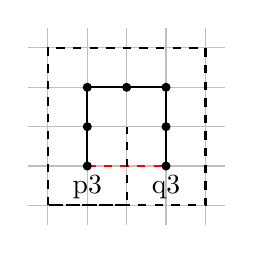
\begin{tikzpicture}
    \draw[step=0.5,lightgray,thin,xshift=-1cm,yshift=-1cm] (0.25,0.25) grid (2.75,2.75);
    \draw[red,dashed,thick] (0,0) -- (1,0);
    \filldraw[black] (0,0) circle (0.05) node[anchor=north] {p3};
    \filldraw[black] (1,0) circle (0.05) node[anchor=north] {q3};
    \foreach \x/\y in {0/1,0/2,1/2,2/2,2/1} {
      \filldraw[black] (0.5*\x,0.5*\y) circle (0.05);
    }
    \draw [thick] (0,0) -- (0,1) -- (1,1) -- (1,0);
    \draw[thick,dashed] (-0.5,-0.5) -- (-0.5,1.5) -- (1.5,1.5) -- (1.5,-0.5) -- (-0.5,-0.5) -- (0.5,-0.5) -- (0.5,0.5);
  \end{tikzpicture} &
  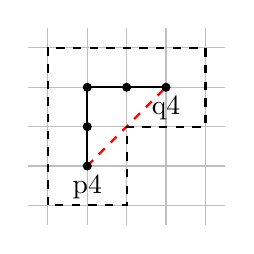
\begin{tikzpicture}
    \draw[step=0.5,lightgray,thin,xshift=-1cm,yshift=-1cm] (0.25,0.25) grid (2.75,2.75);
    \draw[red,dashed,thick] (0,0) -- (1,1);
    \filldraw[black] (0,0) circle (0.05) node[anchor=north] {p4};
    \filldraw[black] (1,1) circle (0.05) node[anchor=north] {q4};
    \foreach \x/\y in {0/1,0/2,1/2} {
      \filldraw[black] (0.5*\x,0.5*\y) circle (0.05);
    }
    \draw [thick] (0,0) -- (0,1) -- (1,1);
    \draw[thick,dashed] (-0.5,-0.5) -- (-0.5,1.5) -- (1.5,1.5) -- (1.5,0.5) -- (0.5,0.5) -- (0.5,-0.5) -- (-0.5,-0.5);
  \end{tikzpicture} \\
  Visible     & Non-Visible                   &
  Non-Visible & Non-Visible
\end{tabular}

%% \begin{tabular}{cc|cc}
%%   \begin{tikzpicture}
%%     \draw[step=0.5,lightgray,thin,xshift=-1cm,yshift=-1cm] (0.25,0.25) grid (3.75,2.75);
%%     \draw[dashed] (0,0) -- (2,1);
%%     \filldraw[black] (0,0) circle (0.05) node[anchor=north] {p1};
%%     \filldraw[black] (2,1) circle (0.05) node[anchor=north] {q1};
%%     \draw [thick] (0,0) -- (0.5,0) -- (1,0) -- (1,0.5) -- (1.5,0.5) -- (1.5,1) -- (2,1);
%%     \draw[thick,dashed] (-0.5,-0.5) -- (-0.5,0.5) -- (0.5,0.5) -- (0.5,1) -- (1,1) -- (1,1.5) -- (2.5,1.5) -- (2.5,0.5) -- (2,0.5) -- (2,0) -- (1.5,0) -- (1.5,-0.5) -- (-0.5,-0.5);
%%   \end{tikzpicture} & & &
%%   \begin{tikzpicture}
%%     \draw[step=0.5,lightgray,thin,xshift=-1cm,yshift=-1cm] (0.25,0.25) grid (3.25,3.25);
%%     \draw[red,dashed,thick] (0,0) -- (1.5,1);
%%     \filldraw[black] (0,0) circle (0.05) node[anchor=north] {p2};
%%     \filldraw[black] (1.5,1) circle (0.05) node[anchor=north] {q2};
%%     \draw [thick] (0,0) -- (0,1) -- (0.5,1) -- (0.5,1.5) -- (1,1.5) -- (1,1) -- (1.5,1);
%%     \draw[thick,dashed] (-0.5,-0.5) -- (-0.5,1.5) -- (0,1.5) -- (0,2) -- (1.5,2) -- (1.5,1.5) -- (2,1.5)  -- (2,0.5) -- (0.5,0.5) -- (0.5,-0.5) -- (-0.5,-0.5);
%%   \end{tikzpicture} \\
%%   Visible                       & & & Non Visible                   \\\\
%%   \hline\\
%%   \begin{tikzpicture}
%%     \draw[step=0.5,lightgray,thin,xshift=-1cm,yshift=-1cm] (0.25,0.25) grid (2.75,2.75);
%%     \draw[red,dashed,thick] (0,0) -- (1,0);
%%     \filldraw[black] (0,0) circle (0.05) node[anchor=north] {p3};
%%     \filldraw[black] (1,0) circle (0.05) node[anchor=north] {q3};
%%     \draw [thick] (0,0) -- (0,1) -- (1,1) -- (1,0);
%%     \draw[thick,dashed] (-0.5,-0.5) -- (-0.5,1.5) -- (1.5,1.5) -- (1.5,-0.5) -- (-0.5,-0.5) -- (0.5,-0.5) -- (0.5,0.5);
%%   \end{tikzpicture} & & &
%%   \begin{tikzpicture}
%%     \draw[step=0.5,lightgray,thin,xshift=-1cm,yshift=-1cm] (0.25,0.25) grid (2.75,2.75);
%%     \draw[red,dashed,thick] (0,0) -- (1,1);
%%     \filldraw[black] (0,0) circle (0.05) node[anchor=north] {p4};
%%     \filldraw[black] (1,1) circle (0.05) node[anchor=north] {q4};
%%     \draw [thick] (0,0) -- (0,1) -- (1,1);
%%     \draw[thick,dashed] (-0.5,-0.5) -- (-0.5,1.5) -- (1.5,1.5) -- (1.5,0.5) -- (0.5,0.5) -- (0.5,-0.5) -- (-0.5,-0.5);
%%   \end{tikzpicture}\\
%%   Non Visible (from a 1-d cell) & & & Non Visible (from a 0-d cell)
%% \end{tabular}

      \caption{Examples of visibility and non visibility in 2D within
        the set $X$ (represented with black disks $\bullet$).}
      \label{fig:visibility-2d}
    \end{figure}


    A quite unexpected fact about visibility it that the set of
    visible points from a source $p$ is not necessarily digitally
    connected in $X$. Indeed, for $n \in \Z, n \Ge 1$, we say that
    $p,q$ are \emph{$n$-neighbors} when $\|q-p\|_\infty \Le n$, and
    this induces the $n$-adjacency and $n$-connectedness relation in
    $X$. As illustrated on
    Figure~\ref{fig:visibility-2d-not-connected}, the set of points
    visible from $p$ is clearly not $1$-connected. As our experiments
    have shown, we even conjecture that it may not be $n$-connected
    for $n$ arbitrarily large.

    This characteristic has implications for the applicability of~\cite[Algorithm 3]{lachaud:2022-jmiv}, which is a breadth-first
    like algorithm for computing all the points of $X$ visible in $X$
    to a source point $p$. This algorithm sometimes outputs an
    incomplete collection of visible points. This is why in the next
    section we present an algorithm that computes the exact visibility
    pairs within $X$, without recourse to connectedness in its formulation.

    %% We note that one particular
    %% aspect of this visibility definition is that all visible points
    %% from a given point taken as a separate complex are not necessarily
    %% 26-connected~\ref{fig:visibility-2d-not-connected}.  Furthermore,
    %% we conjecture that they even may not be $n$-connected for $n$
    %% arbitrarily large.  This characteristic has implications for the
    %% applicability of Algorithm 3 from~\cite{lachaud:2022-jmiv}, as the
    %% algorithm assumes that visited points are 26-connected,
    %% potentially leading to incomplete collection of visible points.

    % Example of visibility not necessarily connected
    % Path from p to q : r u r u r r r r r u r
    \begin{figure}[t]
        \centering
        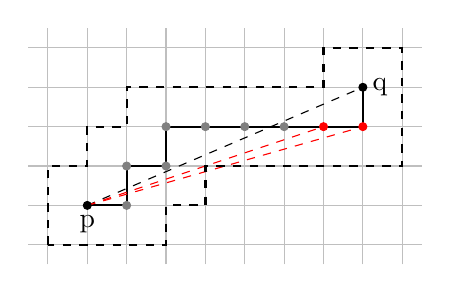
\begin{tikzpicture}
            \draw[step=0.5,lightgray,thin,xshift=-1cm,yshift=-1cm] (0.25,0.25) grid (5.25,3.25);
            \draw[thick] (0,0) -- (0.5,0) -- (0.5,0.5) -- (1,0.5) -- (1,1) -- (3.5,1) -- (3.5,1.5);
            \draw [black, dashed] (0,0) -- (3.5,1.5);
            \draw [red, dashed] (0,0) -- (3.5,1);
            \draw [red, dashed] (0,0) -- (3,1);
            \filldraw[black] (0,0) circle (0.05) node[anchor=north] {p};
            \filldraw[gray] (0.5,0) circle (0.05);
            \filldraw[gray] (0.5,0.5) circle (0.05);
            \filldraw[gray] (1,0.5) circle (0.05);
            \filldraw[gray] (1,1) circle (0.05);
            \filldraw[gray] (1.5,1) circle (0.05);
            \filldraw[gray] (2,1) circle (0.05);
            \filldraw[gray] (2.5,1) circle (0.05);
            \filldraw[red] (3,1) circle (0.05);
            \filldraw[red] (3.5,1) circle (0.05);
            \filldraw[black] (3.5,1.5) circle (0.05) node[anchor=west] {q};
            \draw[thick,dashed] (-0.5,-0.5) -- (-0.5,0.5) -- (0,0.5) -- (0,1) -- (0.5,1) -- (0.5,1.5) -- (3,1.5) -- (3,2) -- (4,2) -- (4,0.5) -- (1.5,0.5) -- (1.5,0) -- (1,0) -- (1,-0.5) -- (-0.5,-0.5);
        \end{tikzpicture}
        \caption{The set of visible points in $X$ from source $p$ is not $1$-connected.}
        \label{fig:visibility-2d-not-connected}
    \end{figure}


%%%%%%%%%%%%%%%%%%%%%%%%%%%%%%%%%%%%%%%%%%%%%%%%%%%%%%%%%%%%%%%%%%%%%%


    \section{Fast computation using integer intervals intersections}

    To improve computation time, we will use lattice maps of integer intervals.

    \begin{definition}
        A sequence of intervals is an ordered list of intervals $L = ([a_i,b_i])_{i=1,\ldots,n}$ such that $b_i + 1 < a_{i+1}$, i.e., disjoint intervals with at least a missing integer.
    \end{definition}

    \begin{definition}
        A translation of an interval $A$ is defined as $A+t \coloneqq [a+t, b+t]$
    \end{definition}

    \begin{definition}
        A translation of a sequence of intervals $L$ is the sequence defined as $L+t \coloneqq \{L_1+t,\ldots,L_n+t\}$
    \end{definition}

    \begin{definition}
        All translations $T$ of an interval or a sequence of intervals $A$ in a sequence of intervals $L$ are defined as $ T \coloneqq \{ t, st. A+t \subset L\}$
    \end{definition}

    We will consider lattice maps as pairs of (shift, intervals), where shifts are points $p \in \R^{d-1}$. All coordinates are doubled, so that the represented cell $\forall c \in \R^d$ will have a dimension equal to $\sum_{i=1}^d \left(c[i]\mod d\right)$.
    In figure~\ref{fig:lattice-representation}, we display a representation of lattice maps applied to a 2-d cell complex where all coordinates are already doubled. Note that the examples are in 2-d, the shown results are in 3-d and the algorithm is for n-d.

    \begin{figure}
        \centering
        \label{fig:lattice-representation}
        % \usetikzlibrary {arrows.meta,decorations.shapes}
        \begin{tabular}{c c}
            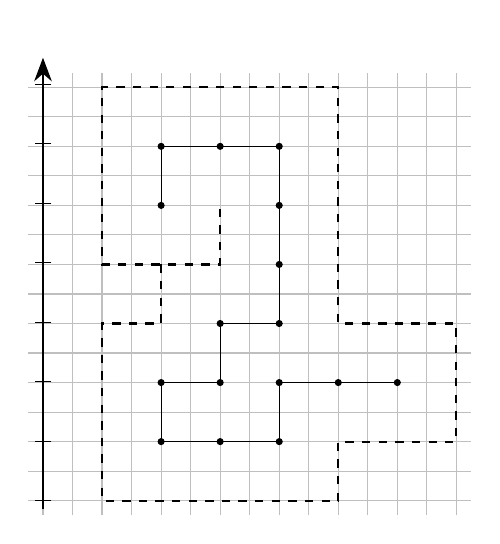
\begin{tikzpicture}[scale=0.75]
                \draw[step=0.5,lightgray,thin,xshift=-1cm,yshift=-1cm] (-0.25,-0.25) grid (7.25,7.25);
                \filldraw[black] (1,4) circle (0.05);
                \filldraw[black] (1,5) circle (0.05);
                \filldraw[black] (2,5) circle (0.05);
                \filldraw[black] (3,5) circle (0.05);
                \filldraw[black] (3,4) circle (0.05);
                \filldraw[black] (3,3) circle (0.05);
                \filldraw[black] (3,2) circle (0.05);
                \filldraw[black] (2,2) circle (0.05);
                \filldraw[black] (2,1) circle (0.05);
                \filldraw[black] (1,1) circle (0.05);
                \filldraw[black] (1,0) circle (0.05);
                \filldraw[black] (2,0) circle (0.05);
                \filldraw[black] (3,0) circle (0.05);
                \filldraw[black] (3,1) circle (0.05);
                \filldraw[black] (4,1) circle (0.05);
                \filldraw[black] (5,1) circle (0.05);
                \draw[-{Stealth[length=3mm]}=black] (-1,-1) -- (-1,6.5);
                \draw decorate [decoration={crosses,transform={rotate=45},shape size=1.5mm,segment length=21.5pt}] {(-1,-1) -- (-1,7)};
                \draw[black] (1,4) -- (1,5) -- (3,5) -- (3,2) -- (2,2) -- (2,1) -- (1,1) -- (1,0) -- (3,0) -- (3,1) -- (5,1);
                \draw[thick,dashed] (1,3) -- (1,2) -- (0,2) -- (0,-1) -- (4,-1) -- (4,0) -- (6,0) -- (6,2) -- (4,2) -- (4,6) -- (0,6) -- (0,3) -- (2,3) -- (2,4);
            \end{tikzpicture} &
            %      \begin{tikzpicture}
            %     \foreach \y in {1,1.5,...,6} {
            %       \draw[thin, lightgray,xshift=-1cm,yshift=-1cm] (0.75,\y) -- (6.25,\y);
            %     }
            %     \draw[-{Stealth[length=3mm]}=black] (0,0) -- (0,5.5);
            %     \draw decorate [decoration={crosses,transform={rotate=45},shape size=1.5mm,segment length=10mm}] {(0,0) -- (0,5)};
            %     \draw[black] (1,4) -- (1,5) -- (3,5) -- (3,2) -- (2,2) -- (2,1) -- (1,1) -- (1,0) -- (3,0) -- (3,1) -- (5,1);
            %     \draw[thick, arrows = {Bracket[sharp]-Bracket[sharp]}] (0.9,5)--(3.1,5);
            %     \draw[thick, arrows = {Bracket[sharp]-Bracket[sharp]}] (0.9,4.5)--(1.1,4.5);
            %     \draw[thick, arrows = {Bracket[sharp]-Bracket[sharp]}] (2.9,4.5)--(3.1,4.5);
            %     \draw[thick, arrows = {Bracket[sharp]-Bracket[sharp]}] (0.9,4)--(1.1,4);
            %     \draw[thick, arrows = {Bracket[sharp]-Bracket[sharp]}] (2.9,4)--(3.1,4);
            %     \draw[thick, arrows = {Bracket[sharp]-Bracket[sharp]}] (2.9,3.5)--(3.1,3.5);
            %     \draw[thick, arrows = {Bracket[sharp]-Bracket[sharp]}] (2.9,3)--(3.1,3);
            %     \draw[thick, arrows = {Bracket[sharp]-Bracket[sharp]}] (2.9,2.5)--(3.1,2.5);
            %     \draw[thick, arrows = {Bracket[sharp]-Bracket[sharp]}] (1.9,2)--(3.1,2);
            %     \draw[thick, arrows = {Bracket[sharp]-Bracket[sharp]}] (1.9,1.5)--(2.1,1.5);
            %     \draw[thick, arrows = {Bracket[sharp]-Bracket[sharp]}] (0.9,1)--(2.1,1);
            %     \draw[thick, arrows = {Bracket[sharp]-Bracket[sharp]}] (2.9,1)--(5.1,1);
            %     \draw[thick, arrows = {Bracket[sharp]-Bracket[sharp]}] (0.9,0.5)--(1.1,0.5);
            %     \draw[thick, arrows = {Bracket[sharp]-Bracket[sharp]}] (2.9,0.5)--(3.1,0.5);
            %     \draw[thick, arrows = {Bracket[sharp]-Bracket[sharp]}] (0.9,0)--(3.1,0);
            %     \filldraw[white,yshift=-1cm] (0,0) circle (0.01); % readjust the height to match the original path
            % \end{tikzpicture} &
            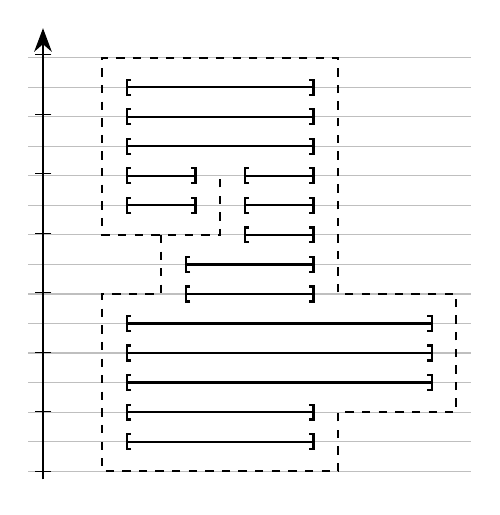
\begin{tikzpicture}[scale=0.75]
                \foreach \y in {0,0.5,...,7} {
                    \draw[thin, lightgray,xshift=-1cm,yshift=-1cm] (-0.25,\y) -- (7.25,\y);
                }
                \draw[-{Stealth[length=3mm]}=black] (-1,-1) -- (-1,6.5);
                \draw decorate [decoration={crosses,transform={rotate=45},shape size=1.5mm,segment length=21.5pt}] {(-1,-1) -- (-1,6.5)};
                \draw[thick,dashed] (1,3) -- (1,2) -- (0,2) -- (0,-1) -- (4,-1) -- (4,0) -- (6,0) -- (6,2) -- (4,2) -- (4,6) -- (0,6) -- (0,3) -- (2,3) -- (2,4);
                \draw[thick, arrows = {Bracket[sharp]-Bracket[sharp]}] (0.4,5.5)--(3.6,5.5);
                \draw[thick, arrows = {Bracket[sharp]-Bracket[sharp]}] (0.4,5)--(3.6,5);
                \draw[thick, arrows = {Bracket[sharp]-Bracket[sharp]}] (0.4,4.5)--(3.6,4.5);
                \draw[thick, arrows = {Bracket[sharp]-Bracket[sharp]}] (0.4,4)--(1.6,4);
                \draw[thick, arrows = {Bracket[sharp]-Bracket[sharp]}] (2.4,4)--(3.6,4);
                \draw[thick, arrows = {Bracket[sharp]-Bracket[sharp]}] (0.4,3.5)--(1.6,3.5);
                \draw[thick, arrows = {Bracket[sharp]-Bracket[sharp]}] (2.4,3.5)--(3.6,3.5);
                \draw[thick, arrows = {Bracket[sharp]-Bracket[sharp]}] (2.4,3)--(3.6,3);
                \draw[thick, arrows = {Bracket[sharp]-Bracket[sharp]}] (1.4,2.5)--(3.6,2.5);
                \draw[thick, arrows = {Bracket[sharp]-Bracket[sharp]}] (1.4,2)--(3.6,2);
                \draw[thick, arrows = {Bracket[sharp]-Bracket[sharp]}] (0.4,1.5)--(5.6,1.5);
                \draw[thick, arrows = {Bracket[sharp]-Bracket[sharp]}] (0.4,1)--(5.6,1);
                \draw[thick, arrows = {Bracket[sharp]-Bracket[sharp]}] (0.4,0.5)--(5.6,0.5);
                \draw[thick, arrows = {Bracket[sharp]-Bracket[sharp]}] (0.4,0)--(3.6,0);
                \draw[thick, arrows = {Bracket[sharp]-Bracket[sharp]}] (0.4,-0.5)--(3.6,-0.5);
                \filldraw[white,yshift=-1.25cm] (0,0) circle (0.01); % readjust the height to match the original path
            \end{tikzpicture}
        \end{tabular}
        \caption{Representation of a 2d cell complex (here the star of a given curve) as a lattice map. From 31 cells from the star on the left, we get 15 intervals on the right}
    \end{figure}

    \colorlet{MyGreen}{green!80!gray}
    \begin{figure}
        \centering
        \begin{tabular}{c c}
            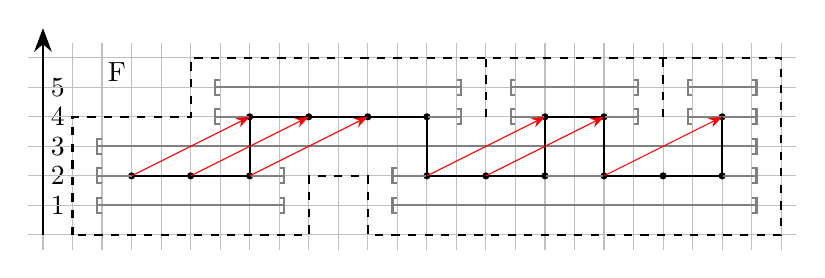
\begin{tikzpicture}[scale=0.75]
                \foreach[count=\i] \y in {-0.5,0,...,1.5} {
                    \draw (0,0) node at (-1.25,\y) {\i};
                }
                \draw[step=0.5,lightgray,thin,xshift=-1cm,yshift=-1cm] (-0.75,-0.25) grid (12.25,3.25);
                \draw[-{Stealth[length=3mm]}=black] (-1.5,-1) -- (-1.5,2.5);
                \filldraw[black] (0,0) circle (0.05);
                \filldraw[black] (1,0) circle (0.05);
                \filldraw[black] (2,0) circle (0.05);
                \filldraw[black] (2,1) circle (0.05);
                \filldraw[black] (3,1) circle (0.05);
                \filldraw[black] (4,1) circle (0.05);
                \filldraw[black] (5,1) circle (0.05);
                \filldraw[black] (5,0) circle (0.05);
                \filldraw[black] (6,0) circle (0.05);
                \filldraw[black] (7,0) circle (0.05);
                \filldraw[black] (7,1) circle (0.05);
                \filldraw[black] (8,1) circle (0.05);
                \filldraw[black] (8,0) circle (0.05);
                \filldraw[black] (9,0) circle (0.05);
                \filldraw[black] (10,0) circle (0.05);
                \filldraw[black] (10,1) circle (0.05);
                \draw[thick,gray, arrows = {Bracket[sharp]-Bracket[sharp]}] (-0.6,-0.5)--(2.6,-0.5);
                \draw[thick,gray, arrows = {Bracket[sharp]-Bracket[sharp]}] (4.4,-0.5)--(10.6,-0.5);
                \draw[thick,gray, arrows = {Bracket[sharp]-Bracket[sharp]}] (-0.6,0)--(2.6,0);
                \draw[thick,gray, arrows = {Bracket[sharp]-Bracket[sharp]}] (4.4,0)--(10.6,0);
                \draw[thick,gray, arrows = {Bracket[sharp]-Bracket[sharp]}] (-0.6,0.5)--(10.6,0.5);
                \draw[thick,gray, arrows = {Bracket[sharp]-Bracket[sharp]}] (1.4,1)--(5.6,1);
                \draw[thick,gray, arrows = {Bracket[sharp]-Bracket[sharp]}] (6.4,1)--(8.6,1);
                \draw[thick,gray, arrows = {Bracket[sharp]-Bracket[sharp]}] (9.4,1)--(10.6,1);
                \draw[thick,gray, arrows = {Bracket[sharp]-Bracket[sharp]}] (1.4,1.5)--(5.6,1.5);
                \draw[thick,gray, arrows = {Bracket[sharp]-Bracket[sharp]}] (6.4,1.5)--(8.6,1.5);
                \draw[thick,gray, arrows = {Bracket[sharp]-Bracket[sharp]}] (9.4,1.5)--(10.6,1.5);
                \draw[thick, black] (0,0) -- (2,0) -- (2,1) -- (5,1) -- (5,0) -- (7,0) -- (7,1) -- (8,1) -- (8,0) -- (10,0) -- (10,1);
                \draw[thick,dashed] (6,1) -- (6,2);
                \draw[thick,dashed] (9,1) -- (9,2);
                \draw[thick,dashed] (-1,-1) -- (-1,1) -- (1,1) -- (1,2) -- (11,2) -- (11,-1) -- (4,-1) -- (4,0) -- (3,0) -- (3,-1) -- (-1,-1);

                \draw (0,0) node at (-0.25,1.75) {F};

                \draw[red,arrows = {-Stealth[]}] (0,0)--(2,1);
                \draw[red,arrows = {-Stealth[]}] (1,0)--(3,1);
                \draw[red,arrows = {-Stealth[]}] (2,0)--(4,1);
                \draw[red,arrows = {-Stealth[]}] (5,0)--(7,1);
                \draw[red,arrows = {-Stealth[]}] (6,0)--(8,1);
                \draw[red,arrows = {-Stealth[]}] (8,0)--(10,1);


            \end{tikzpicture} &
            \begin{tikzpicture}[scale=0.75]
                \draw[step=0.5,lightgray,thin,xshift=-1cm,yshift=-1cm] (-0.75,-0.25) grid (4.25,3.25);
                \draw[-{Stealth[length=3mm]}=black] (-1.5,-1) -- (-1.5,2.5);
                \foreach[count=\i] \y in {-0.5,0,...,1.5} {
                    \draw (0,0) node at (-1.25,\y) {\i};
                }
                \filldraw[black] (0,0) circle (0.05);
                \filldraw[black] (2,1) circle (0.05);
                \draw[thick, black] (0,0) -- (2,1);
                \draw[thick,dashed] (-1,-1) -- (-1,1) -- (1,1) -- (1,2) -- (3,2) -- (3,0) -- (1,0) --  (1,-1) -- (-1,-1);
                \draw[thick,MyGreen, arrows = {Bracket[sharp]-Bracket[sharp]}] (-0.6,-0.5)--(0.6,-0.5);
                \draw[thick,MyGreen, arrows = {Bracket[sharp]-Bracket[sharp]}] (-0.6,0)--(0.6,0);
                \draw[thick,MyGreen, arrows = {Bracket[sharp]-Bracket[sharp]}] (-0.6,0.5)--(2.6,0.5);
                \draw[thick,MyGreen, arrows = {Bracket[sharp]-Bracket[sharp]}] (1.4,1)--(2.6,1);
                \draw[thick,MyGreen, arrows = {Bracket[sharp]-Bracket[sharp]}] (1.4,1.5)--(2.6,1.5);

                \draw (0,0) node at (-0.25,1.75) {V};
            \end{tikzpicture} \\
            \hline
            \multicolumn{2}{c}{
                \begin{tikzpicture}[scale=0.75]
                    \foreach \y in {0,0.5,...,12.5} {
                        \draw[thin, lightgray] (-1.25,\y) -- (11.25,\y);
                    }
                    \foreach \y in {0,2.5,...,12.5} {
                        \draw[blue] (-7,\y) -- (11.25,\y);
                    }

                    \foreach[count=\i] \y in {12,9.5,...,2} {
                        \draw (0,0) node at (-4,\y) {$V_{\i}$};
                    }
                    \foreach[count=\i] \y in {11.5,9,...,1.5} {
                        \draw (0,0) node at (-4,\y) {$F_{\i}$};
                    }
                    \draw (0,0) node at (-4,11) {$T_{1} = \text{Translations}(V_{1},F_{1})$};
                    \foreach[count=\i] \y in {8.5,6,...,1} {
                        \draw (0,0) node at (-4,\y) {$T_{\the\numexpr\i+1\relax}$};
                    }
                    \draw (0,0) node at (-4,10.5) {$R_1 = T_1$};

                    \foreach[count=\i] \y in {8,5.5,...,0.5} {

                        \draw (0,0) node at (-4,\y) {$R_{\the\numexpr\i+1\relax} = T_{\the\numexpr\i+1\relax} \cap R_{\i}$};
                    }

                    \draw[thick,MyGreen,arrows = {Bracket[sharp]-Bracket[sharp]}] (-0.6,12)--(0.6,12);
                    \draw[thick,gray,arrows = {Bracket[sharp]-Bracket[sharp]}] (-0.6,11.5)--(2.6,11.5);
                    \draw[thick,gray,arrows = {Bracket[sharp]-Bracket[sharp]}] (4.4,11.5)--(10.6,11.5);
                    \draw[thick,violet,arrows = {Bracket[sharp]-Bracket[sharp]}] (-0.6,11)--(1.6,11);
                    \draw[thick,violet,arrows = {Bracket[sharp]-Bracket[sharp]}] (4.4,11)--(9.6,11);
                    \draw[thick,red,arrows = {Bracket[sharp]-Bracket[sharp]}] (-0.6,10.5)--(1.6,10.5);
                    \draw[thick,red,arrows = {Bracket[sharp]-Bracket[sharp]}] (4.4,10.5)--(9.6,10.5);
                    \filldraw[black] (-0.5,10.5) circle (0.05);
                    \filldraw[black] (0.5,10.5) circle (0.05);
                    \filldraw[black] (1.5,10.5) circle (0.05);
                    \filldraw[black] (4.5,10.5) circle (0.05);
                    \filldraw[black] (5.5,10.5) circle (0.05);
                    \filldraw[black] (6.5,10.5) circle (0.05);
                    \filldraw[black] (7.5,10.5) circle (0.05);
                    \filldraw[black] (8.5,10.5) circle (0.05);
                    \filldraw[black] (9.5,10.5) circle (0.05);


                    \draw[thick,MyGreen,arrows = {Bracket[sharp]-Bracket[sharp]}] (-0.6,9.5)--(0.6,9.5);
                    \draw[thick,gray,arrows = {Bracket[sharp]-Bracket[sharp]}] (-0.6,9)--(2.6,9);
                    \draw[thick,gray,arrows = {Bracket[sharp]-Bracket[sharp]}] (4.4,9)--(10.6,9);
                    \draw[thick,violet,arrows = {Bracket[sharp]-Bracket[sharp]}] (-0.6,8.5)--(1.6,8.5);
                    \draw[thick,violet,arrows = {Bracket[sharp]-Bracket[sharp]}] (4.4,8.5)--(9.6,8.5);
                    \draw[thick,red,arrows = {Bracket[sharp]-Bracket[sharp]}] (-0.6,8)--(1.6,8);
                    \draw[thick,red,arrows = {Bracket[sharp]-Bracket[sharp]}] (4.4,8)--(9.6,8);
                    \filldraw[black] (-0.5,8) circle (0.05);
                    \filldraw[black] (0.5,8) circle (0.05);
                    \filldraw[black] (1.5,8) circle (0.05);
                    \filldraw[black] (4.5,8) circle (0.05);
                    \filldraw[black] (5.5,8) circle (0.05);
                    \filldraw[black] (6.5,8) circle (0.05);
                    \filldraw[black] (7.5,8) circle (0.05);
                    \filldraw[black] (8.5,8) circle (0.05);
                    \filldraw[black] (9.5,8) circle (0.05);

                    \draw[thick,MyGreen,arrows = {Bracket[sharp]-Bracket[sharp]}] (-0.6,7)--(2.6,7);
                    \draw[thick,gray,arrows = {Bracket[sharp]-Bracket[sharp]}] (-0.6,6.5)--(10.6,6.5);
                    \draw[thick,violet,arrows = {Bracket[sharp]-Bracket[sharp]}] (-0.6,6)--(7.6,6);
                    \draw[thick,red,arrows = {Bracket[sharp]-Bracket[sharp]}] (-0.6,5.5)--(1.6,5.5);
                    \draw[thick,red,arrows = {Bracket[sharp]-Bracket[sharp]}] (4.4,5.5)--(7.6,5.5);
                    \filldraw[black] (-0.5,5.5) circle (0.05);
                    \filldraw[black] (0.5,5.5) circle (0.05);
                    \filldraw[black] (1.5,5.5) circle (0.05);
                    \filldraw[black] (4.5,5.5) circle (0.05);
                    \filldraw[black] (5.5,5.5) circle (0.05);
                    \filldraw[black] (6.5,5.5) circle (0.05);
                    \filldraw[black] (7.5,5.5) circle (0.05);

                    \draw[thick,black,arrows = {-Stealth[]}] (-0.6,4.5)--(1.4,4.5);
                    \draw[thick,MyGreen,arrows = {Bracket[sharp]-Bracket[sharp]}] (1.4,4.5)--(2.6,4.5);
                    \draw[thick,gray,arrows = {Bracket[sharp]-Bracket[sharp]}] (1.4,4)--(5.6,4);
                    \draw[thick,gray,arrows = {Bracket[sharp]-Bracket[sharp]}] (6.4,4)--(8.6,4);
                    \draw[thick,gray,arrows = {Bracket[sharp]-Bracket[sharp]}] (9.4,4)--(10.6,4);
                    \draw[thick,violet,arrows = {Bracket[sharp]-Bracket[sharp]}] (-0.6,3.5)--(2.6,3.5);
                    \draw[thick,violet,arrows = {Bracket[sharp]-Bracket[sharp]}] (4.4,3.5)--(5.6,3.5);
                    \draw[thick,violet,arrows = {Bracket[sharp]-Bracket[sharp]}] (7.4,3.5)--(7.6,3.5);
                    \draw[thick,red,arrows = {Bracket[sharp]-Bracket[sharp]}] (-0.6,3)--(1.6,3);
                    \draw[thick,red,arrows = {Bracket[sharp]-Bracket[sharp]}] (4.4,3)--(5.6,3);
                    \draw[thick,red,arrows = {Bracket[sharp]-Bracket[sharp]}] (7.4,3)--(7.6,3);
                    \filldraw[black] (-0.5,3) circle (0.05);
                    \filldraw[black] (0.5,3) circle (0.05);
                    \filldraw[black] (1.5,3) circle (0.05);
                    \filldraw[black] (4.5,3) circle (0.05);
                    \filldraw[black] (5.5,3) circle (0.05);
                    \filldraw[black] (7.5,3) circle (0.05);

                    \draw[thick,black,arrows = {-Stealth[]}] (-0.6,2)--(1.4,2);
                    \draw[thick,MyGreen,arrows = {Bracket[sharp]-Bracket[sharp]}] (1.4,2)--(2.6,2);
                    \draw[thick,gray,arrows = {Bracket[sharp]-Bracket[sharp]}] (1.4,1.5)--(5.6,1.5);
                    \draw[thick,gray,arrows = {Bracket[sharp]-Bracket[sharp]}] (6.4,1.5)--(8.6,1.5);
                    \draw[thick,gray,arrows = {Bracket[sharp]-Bracket[sharp]}] (9.4,1.5)--(10.6,1.5);
                    \draw[thick,violet,arrows = {Bracket[sharp]-Bracket[sharp]}] (-0.6,1)--(2.6,1);
                    \draw[thick,violet,arrows = {Bracket[sharp]-Bracket[sharp]}] (4.4,1)--(5.6,1);
                    \draw[thick,violet,arrows = {Bracket[sharp]-Bracket[sharp]}] (7.4,1)--(7.6,1);
                    \draw[thick,red,arrows = {Bracket[sharp]-Bracket[sharp]}] (-0.6,0.5)--(1.6,0.5);
                    \draw[thick,red,arrows = {Bracket[sharp]-Bracket[sharp]}] (4.4,0.5)--(5.6,0.5);
                    \draw[thick,red,arrows = {Bracket[sharp]-Bracket[sharp]}] (7.4,0.5)--(7.6,0.5);
                    \filldraw[black] (-0.5,0.5) circle (0.05);
                    \filldraw[black] (0.5,0.5) circle (0.05);
                    \filldraw[black] (1.5,0.5) circle (0.05);
                    \filldraw[black] (4.5,0.5) circle (0.05);
                    \filldraw[black] (5.5,0.5) circle (0.05);
                    \filldraw[black] (7.5,0.5) circle (0.05);

                \end{tikzpicture}}
        \end{tabular}
        \caption{Evolution of the visibility check algorithm for a 2,1 vector. Green is the vector lattice map, black is the figure lattice map, red are the current intervals of positions where the visibility is still possible. The last red intervals are the visible positions. We travel the lattice maps from bottom-up. The found possible visibilities are shown on the original figure}
        \label{fig:visibility-algorithm-evolution}
    \end{figure}

    \begin{algorithm}
        \caption{Given a cell complex C and a radius $r$, compute the visibility at every point of C up to distance $r$. We assume z being the main axis of the lattice maps, x and y being the auxiliary axises}
        \label{alg:visibility}
        \begin{algorithmic}
            \Function{Visibility}{C: Cell complex, r: Integer}
                \State $\Omega \gets \Call{Star}{C}$ \Comment{Lattice map of the star of the studied cell complex}
                \State $Directions \gets \Call{GetAllPrimalDirections}{r}$
                \State $V: \text{vector of boolean} \gets [0, \ldots, 0]$ \Comment{length $Size(Directions) \times \#C.pointels$}
                \State $low, high \gets \Call{BoundingBoxZ}{\Omega}$
                \ForAll{$d$ in $Directions$}
                    \ForAll{shift $S$ in $\Omega$}
                        \State $R \gets [low, high]$
                        \ForAll{pair $P$ in $\Call{Star}{\text{d}}$}
                            \State $R \gets R \cap \Call{Translations}{P.intervals,\Omega[S + P.shift]}$
                        \EndFor
                        \State \Call{UpdateVisibility}{$V$, $R$}
                    \EndFor
                \EndFor
                \State \Return $V$
            \EndFunction
        \end{algorithmic}
    \end{algorithm}

    In order to compute the visibility, we first compute $\Omega = \text{Star}(C)$. Then for each primal direction of
    coordinates at most $r$, we look at all the possible positions this specific direction does link 2 visible points
    of the cell complex. In order to do so, for each shift in $\Omega$, we compute the positions where points are
    visible using the same method as presented in~\ref{fig:visibility-algorithm-evolution}. Some results of visible
    points are present in figure~\ref{fig:visibility-results}.

    \begin{algorithm}
        \caption{Given 2 lists of intervals $K$ and $L$, find $K \cap L$, the intersection of those 2 lists}
        \label{alg:intersection}
        \begin{algorithmic}
            \Function{Intersection ($\cap$)}{\text{K, L}: Intervals}
                \State $R \gets \emptyset$; $k, l \gets 0$
                \While{$k < K.nbIntervals \And l < L.nbIntervals$}
                    \State $[a,b] \gets K[k]$; $[c,d] \gets L[l]$
                    \State $e \gets \max(a, c)$; $f \gets \min(b, d)$
                    \If{$e \leq f$}
                        \State $R.append([e, f])$
                    \EndIf
                    \If{$b \leq d$}
                        \State $k \gets k+1$
                    \EndIf
                    \If{$d \leq b$}
                        \State $l \gets l+1$
                    \EndIf
                \EndWhile
                \State \Return $R$
            \EndFunction
        \end{algorithmic}
    \end{algorithm}

    To efficiently compute the intersection of 2 lists of intervals $K$ and $L$, we go through the first 2 unvisited
    elements of the 2 lists. If they don't overlap (i.e.\ the start and end of the 1st interval are both smaller than
    the start of the other), then we can discard the smaller interval. Else, we construct the intersection of these
    2 intervals as one of the resulting intervals. We then can skip the interval with the smallest end. If both
    intervals have the same end, then both intervals can be skipped. Doing this computation until one of the lists
    is empty returns the intersection of both lists of intervals.

    % Insert visibility results images

    \begin{figure}
        \centering
        \begin{tabular}{c c}
            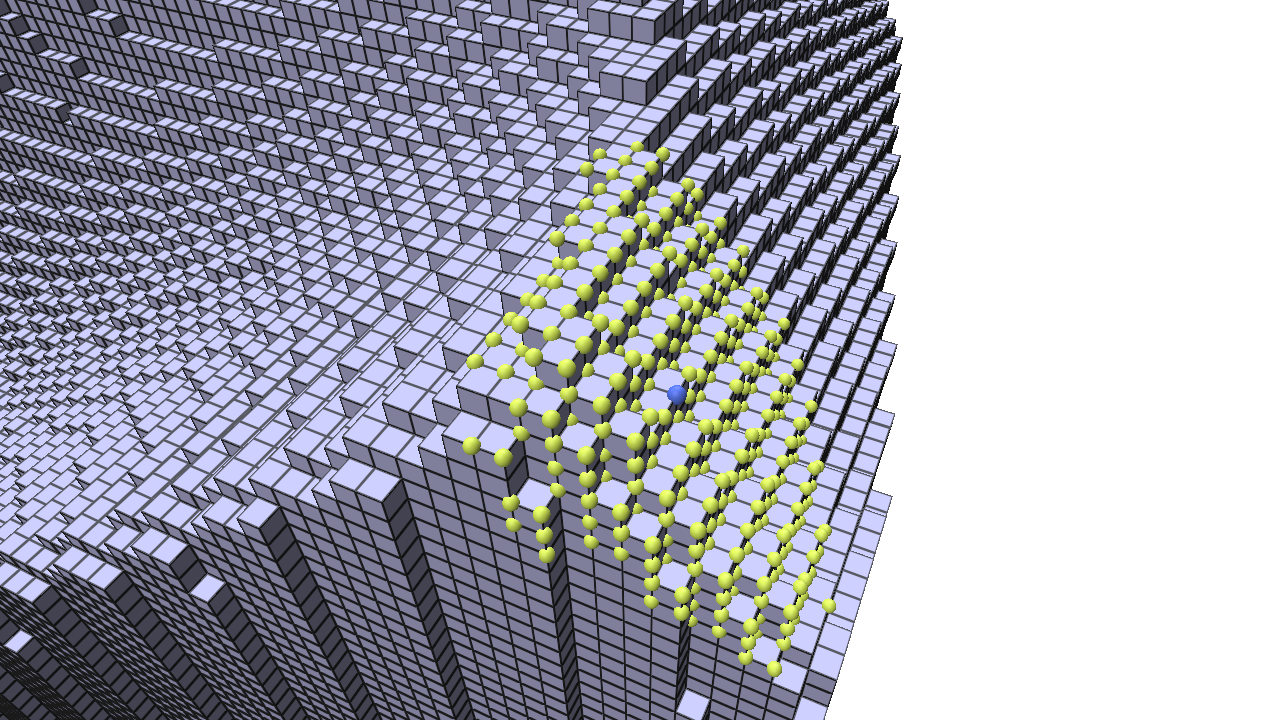
\includegraphics[width=0.4\textwidth]{pictures/visibility_from_given_point_r_10} &
            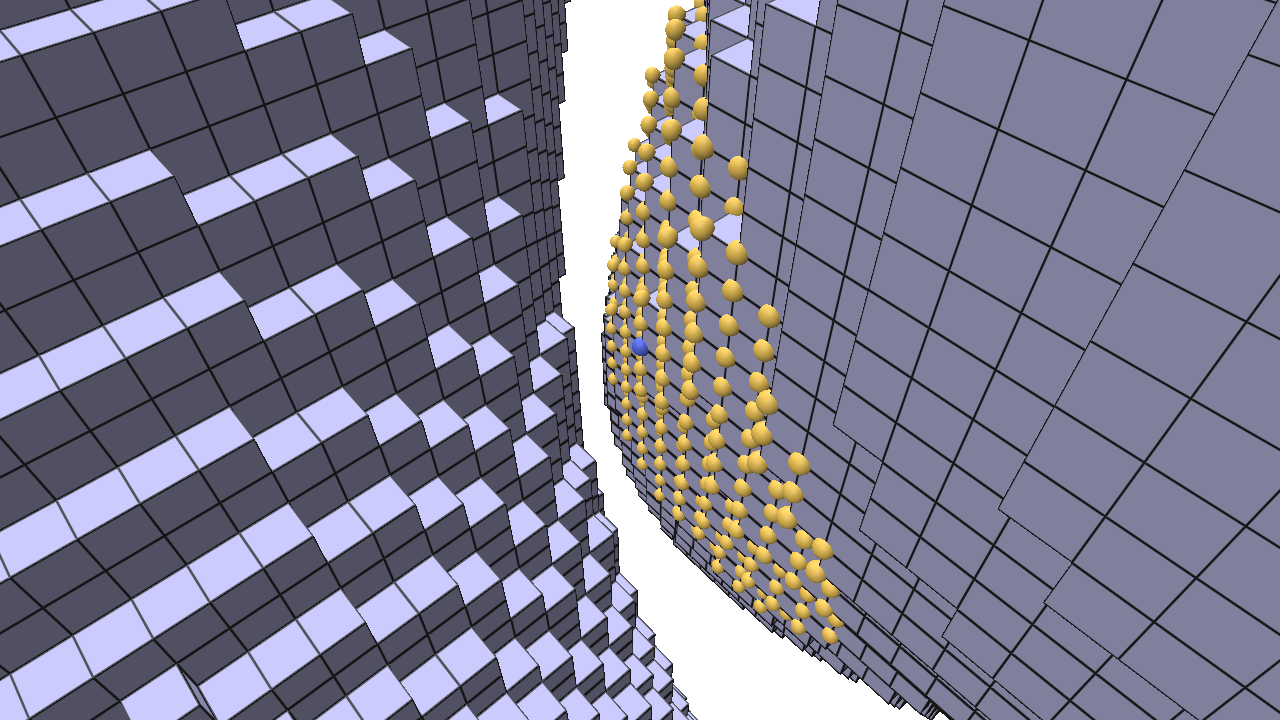
\includegraphics[width=0.4\textwidth]{pictures/visibility_aware_of_features}
        \end{tabular}
        \caption{Examples of visibility on a fandisk and a torus knot. First one is on the edge
        of a fandisk, where the visibility stops at the edges. The other one is in the interior
        of a torus knot, where we can see that the visibility is feature-aware and doesn't see
        the other side of the torus' branch.}
        \label{fig:visibility-results}
    \end{figure}
%
%    \begin{figure}
%        \begin{center}
%            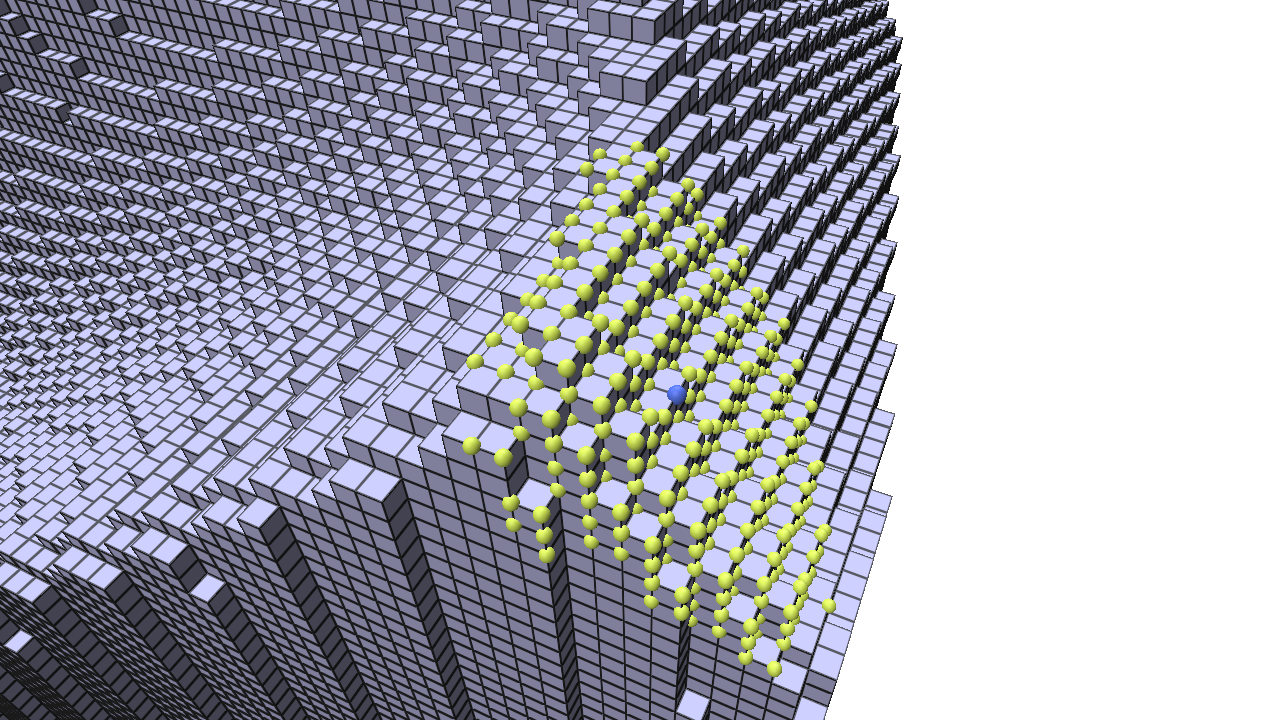
\includegraphics[width=0.8\textwidth]{pictures/visibility_from_given_point_r_10}
%            \caption{Visibility of a point on an edge of a fandisk}
%            \label{fig:visibility-fandisk}
%        \end{center}
%    \end{figure}
%    \begin{figure}
%        \begin{center}
%            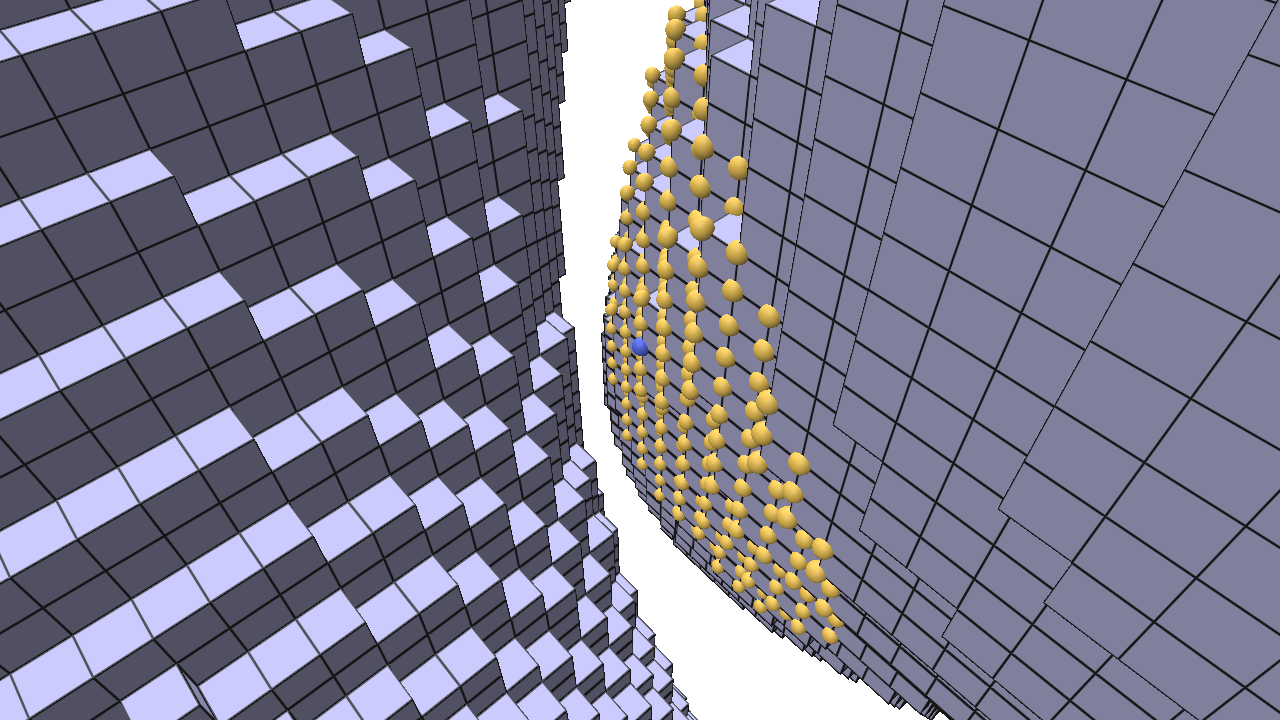
\includegraphics[width=0.8\textwidth]{pictures/visibility_aware_of_features}
%            \caption{Visibility of a point on a torus knot (the visibility is feature-aware)}
%            \label{fig:visibility-torus-knot}
%        \end{center}
%    \end{figure}


    % Quantitative results

    \begin{figure}
        \begin{tikzpicture}
            \centering
            \begin{axis}[
                width=0.8\textwidth,
                legend columns=3,
                xlabel={Gridstep},
                ylabel={Mean distance},
                x dir=reverse,
                legend pos=north west,
                ymajorgrids=true,
                grid style=dashed,
                ymax=50,
                ymode=log,
                xmode=log,
                log ticks with fixed point,
            ]

                \addplot[
                    color=cyan,
                ] coordinates {
                    (0.0625,7.61948)(0.125,5.49755)(0.25,3.97418)(0.375,3.00921)(0.5,2.85702)(0.625,2.34448)(0.75,1.85023)(0.875,2.16868)(1.0,1.85023)
                };
                \addlegendentry{sphere1}
                \addplot[
                    color=red,
                ] coordinates {
                    (0.0625,38.1045)(0.125,26.8765)(0.25,19.6747)(0.375,16.6192)(0.5,14.0867)(0.625,12.5062)(0.75,11.3734)(0.875,10.2845)(1,8.90781)
                };
                \addlegendentry{goursat}
                \addplot[
                    color=violet,
                ] coordinates {
                    (0.0625,25.5024)(0.125,18.2364)(0.25,12.3975)(0.375,9.41303)(0.5,8.69558)(0.625,7.37667)(0.75,6.82131)(0.875,6.05735)(1,6.33877)
                };
                \addlegendentry{torus}
                \addplot[
                    color=MyGreen,
                ] coordinates {
                    (0.0625,27.9287)(0.125,17.5104)(0.25,10.8007)(0.375,8.69514)(0.5,7.26074)(0.625,6.2309)(0.75,5.6897)(0.875,5.28197)(1,4.96098)
                };
                \addlegendentry{leopold}
                \addplot[
                    color=yellow!80!black,
                ] coordinates {
                    (0.0625,41.9816)(0.125,27.7104)(0.25,18.2339)(0.375,14.6475)(0.5,12.3618)(0.625,9.55647)(0.75,9.83208)(0.875,7.51861)(1,7.99732)
                };
                \addlegendentry{rcube}
                \addplot [
                    color=black,
                    thick,
                    domain=0.25:1,
                    samples=100,
                ] {x^(-0.5)};
                \addlegendentry{$\sqrt{h}=\sqrt{\frac{1}{x}}$}
            \end{axis}
        \end{tikzpicture}
        \caption{Mean Visibility Distance as a Function of Grid Resolution}
        \label{fig:meanvisibility-gridstep}
    \end{figure}
    \begin{figure}
        \begin{tikzpicture}
            \centering
            \begin{axis}[
                width=0.8\textwidth,
                xlabel={\#Pointels},
                ylabel={Computation Time (ms)},
                legend pos=north west,
                ymajorgrids=true,
                grid style=dashed,
                ymode=log,
                xmode=log,
                log ticks with fixed point,
            ]
                \addplot[
                    red,
                    only marks,
                    mark=halfcircle,
                    mark options={solid}
                ] table[row sep=crcr] {
                    10624 2246.69\\
                    4968 793.426\\
                    2584 328.535\\
                    1840 190.401\\
                    1176 93.2502\\
                    912 78.7981\\
                    624 56.3769\\
                    28568 10193.5\\
                    12632 4004.92\\
                    7088 2010.63\\
                    4664 1188.73\\
                    3080 755.754\\
                    2408 545.347\\
                    1736 366.541\\
                    24320 11169.1\\
                    10760 4720.44\\
                    6056 2397.79\\
                    3944 1380.38\\
                    2648 874.979\\
                    2000 580.0\\
                    1520 415.373\\
                    8336 3196.55\\
                    3720 1268.46\\
                    2104 639.305\\
                    1336 342.873\\
                    928 177.54\\
                    680 112.142\\
                    520 87.0747\\
                    37592 12335.6\\
                    16712 5582.38\\
                    9512 2976.21\\
                    6056 1731.32\\
                    4088 990.78\\
                    3032 788.507\\
                    2456 548.66\\
                    97844 49226.3\\
                    390235 181322\\
                };
                \addlegendentry{radius 10};
                \addplot[
                    MyGreen,
                    only marks,
                    mark=halfcircle,
                    mark options={solid}
                ] table[row sep=crcr] {
                    10624 9522.43\\
                    4968 2876.81\\
                    2584 1152.25\\
                    1840 635.332\\
                    1176 347.973\\
                    912 304.801\\
                    624 250.126\\
                    28568 70137.9\\
                    12632 26063.0\\
                    7088 11985.8\\
                    4664 6239.51\\
                    3080 3468.31\\
                    2408 2059.84\\
                    1736 1254.2\\
                    24320 86616.9\\
                    10760 26605.7\\
                    6056 11813.5\\
                    3944 6516.92\\
                    2648 3564.03\\
                    2000 1949.32\\
                    1520 1244.89\\
                    8336 18125.5\\
                    3720 5157.11\\
                    2104 2029.09\\
                    1336 896.186\\
                    928 446.136\\
                    680 306.651\\
                    520 259.078\\
                    37592 76316.3\\
                    16712 27747.3\\
                    9512 13608.6\\
                    6056 7140.03\\
                    4088 3704.52\\
                    3032 2624.2\\
                    2456 1422.6\\
                    97844 378906\\
                    390235 1747780\\
                };
                \addlegendentry{radius 20};
                \addplot[
                    blue,
                    only marks,
                    mark=halfcircle,
                    mark options={solid}
                ] table[row sep=crcr] {
                    10624 18283.5\\
                    4968 4957.93\\
                    2584 2133.36\\
                    1840 1292.53\\
                    1176 922.51\\
                    912 863.731\\
                    624 813.638\\
                    28568 188784.0\\
                    12632 62237.1\\
                    7088 24874.9\\
                    4664 9043.39\\
                    3080 4407.09\\
                    2408 2641.04\\
                    1736 1820.31\\
                    24320 227432.0\\
                    10760 69706.8\\
                    6056 25408.9\\
                    3944 10094.7\\
                    2648 5269.56\\
                    2000 2948.16\\
                    1520 2082.02\\
                    8336 45045.4\\
                    3720 8638.42\\
                    2104 3238.48\\
                    1336 1731.9\\
                    928 1122.69\\
                    680 928.084\\
                    520 890.592\\
                    37592 257981.0\\
                    16712 84729.7\\
                    9512 36298.8\\
                    6056 15640.2\\
                    4088 6662.17\\
                    3032 4431.71\\
                    2456 2621.98\\
                    97844 1157400\\
                    390235 10493200\\
                };
                \addlegendentry{radius 30};
                \addplot[
                    orange,
                    only marks,
                    mark=square,
                    mark options={solid}
                ] table[row sep=crcr] {
                    % torus
                    10624 7172.49\\
                    4968 2330.69\\
                    2584 883.559\\
                    1840 568.776\\
                    1176 278.712\\
                    912 212.285\\
                    624 122.615\\
                    % rcube
                    28568 20358.9\\
                    12632 5964.1\\
                    7088 2631.15\\
                    4664 1394.49\\
                    3080 742.638\\
                    2408 554.389\\
                    1736 334.654\\
                    % sphere9
                    24320 21263.4\\
                    10760 6225.27\\
                    6056 2829.2\\
                    3944 1494.98\\
                    2648 833.047\\
                    2000 579.561\\
                    1520 394.169\\
                    % leopold
                    8336 6866.82\\
                    3720 2232.34\\
                    2104 1050.28\\
                    1336 576.853\\
                    928 354.691\\
                    680 243.249\\
                    520 174.452\\
                    % goursat
                    37592 26954.6\\
                    16712 8358.2\\
                    9512 3748.3\\
                    6056 1921.43\\
                    4088 1088.38\\
                    3032 706.378\\
                    2456 531.932\\
                    % d20
                    97844 26392.3\\
                    390235 110416.0\\
                };
                \addlegendentry{naive breadth first};
                \addplot [
                    color=black,
                    thick,
                    domain=500:60000,
                    samples=100,
                ] {0.01*x^(1.5)};
                \addlegendentry{$0.01\times x\sqrt{x}$}
            \end{axis}
        \end{tikzpicture}
        \caption{Computation Time of Visibility as a Function of Grid Resolution}
        \label{fig:meanvisibility-computationComplexity}
    \end{figure}


%%%%%%%%%%%%%%%%%%%%%%%%%%%%%%%%%%%%%%%%%%%%%%%%%%%%%%%%%%%%%%%%%%%%%%


    \section{Saliency-aware normal and curvature estimation}

    \newcommand{\Kernel}[1]{\ensuremath{w_{\sigma}(#1)}}

    \paragraph{Saliency-aware normal estimator.}
    We propose a new normal estimator on digital surfaces, which uses
    the visibility of the point of interest while taking into account
    a user-given scale $\sigma$. If $\sigma$ is proportionnal to the
    average length between visible points (so some
    $\Theta\left(\sqrt{h}\right)$), then this estimator is observed to be
    multigrid convergent along digitization of smooth shapes. However,
    since the computation window is limited by the visibility, it
    better approximates the geometry near sharp or salient features.

    More precisely, we choose a Gaussian function
    $\Kernel{x}\coloneqq e^{-\frac{x^2}{2\sigma^2}}$ as a weight kernel. Let
    $V_p$ be the set of visible points from the point $p$. Let $c_p$
    be the weighted centroid of the visible points around $p$,
    i.e. $c_p \coloneqq \frac{\sum_{q \in V_p} \Kernel{\|q-p\|}q}{\sum_{q \in
    V_p} \Kernel{\|q-p\|}}$. We form the weighted covariance matrix
    $\mathcal{V}_p$ of the points $V_p$ as:
    \begin{equation}
        \mathcal{V}_p = \sum_{q \in V_p} \Kernel{\|q-p\|}(q - c_p)(q - c_p)^T.
    \end{equation}
    The \emph{visibility normal} $\vec{n}(p)$ of point $p$ at scale $\sigma$ is defined
    as the first eigenvector of the covariance matrix $\mathcal{V}_p$
    of the visible points, corresponding to its smallest
    eigenvalue. Its orientation is chosen so as to point in the same
    direction as the average of the trivial normals to the surfels
    touching the point $p$.


    \paragraph{Experimental validation.} [TO COMPLETE]
    Figure~\ref{fig:normals-estimation} shows an example
    of our normals compared to normals computed with the integral invariant (II) estimator~\cite{Lachaud:2017-lnm}.

    \begin{figure}
        \centering
        \begin{tabular}{|c||c|c|}
            \hline
            Normals & With cube edges & Flat (no shading) \\
            \hline
            \hline
            \raisebox{18mm}{II} &
            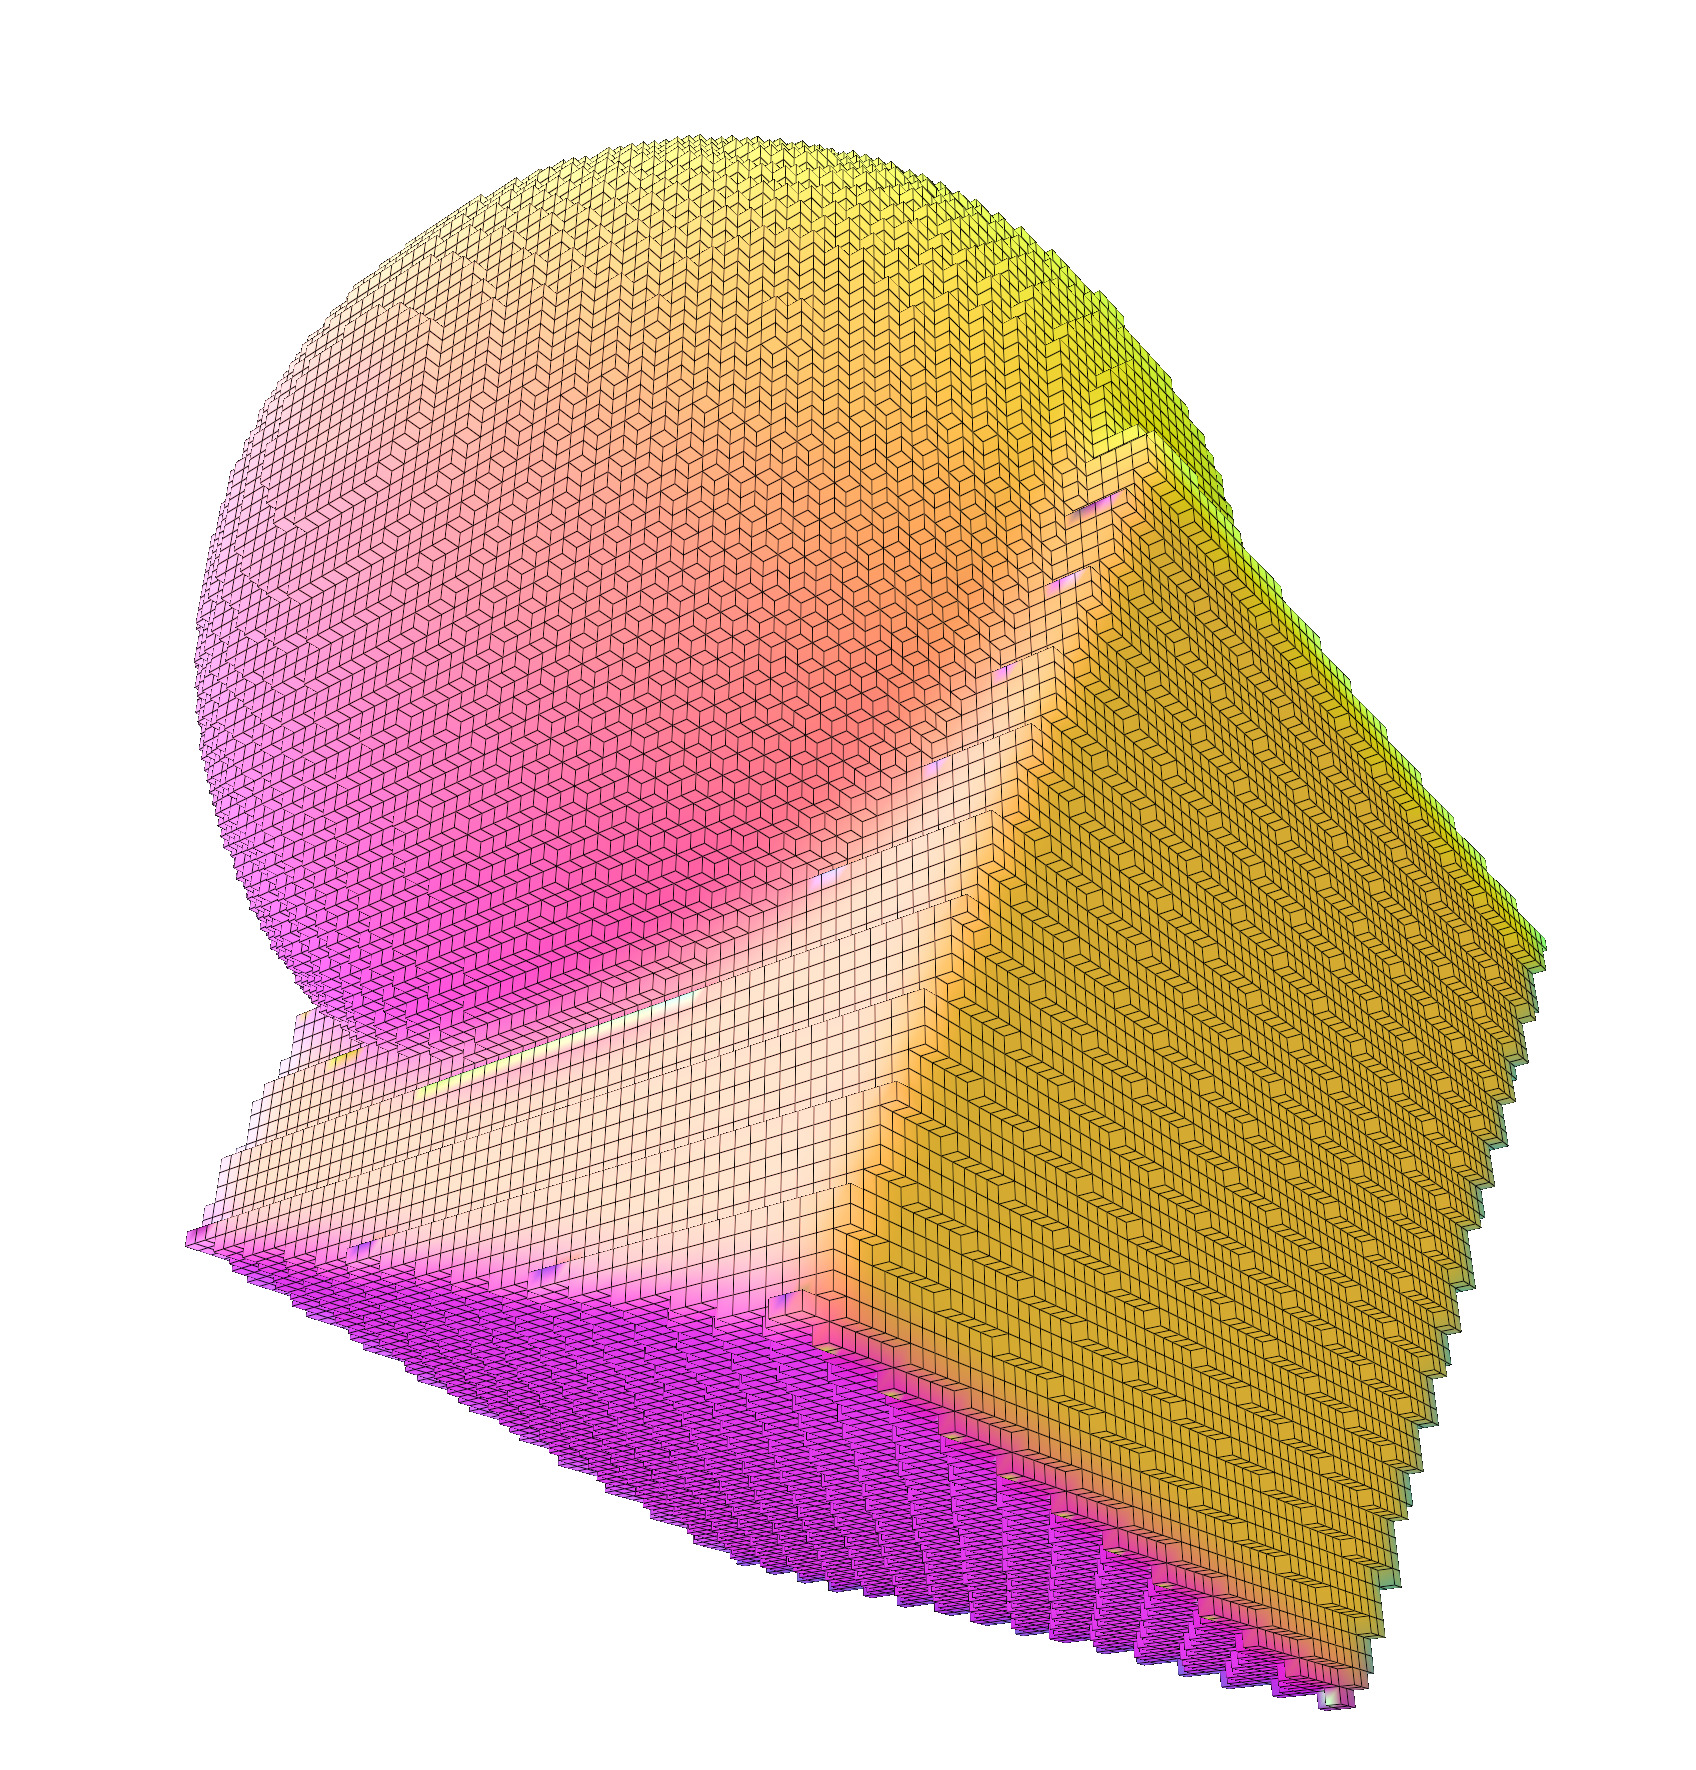
\includegraphics[width=0.3\textwidth]{pictures/cps-IIN-flat-edge} &
            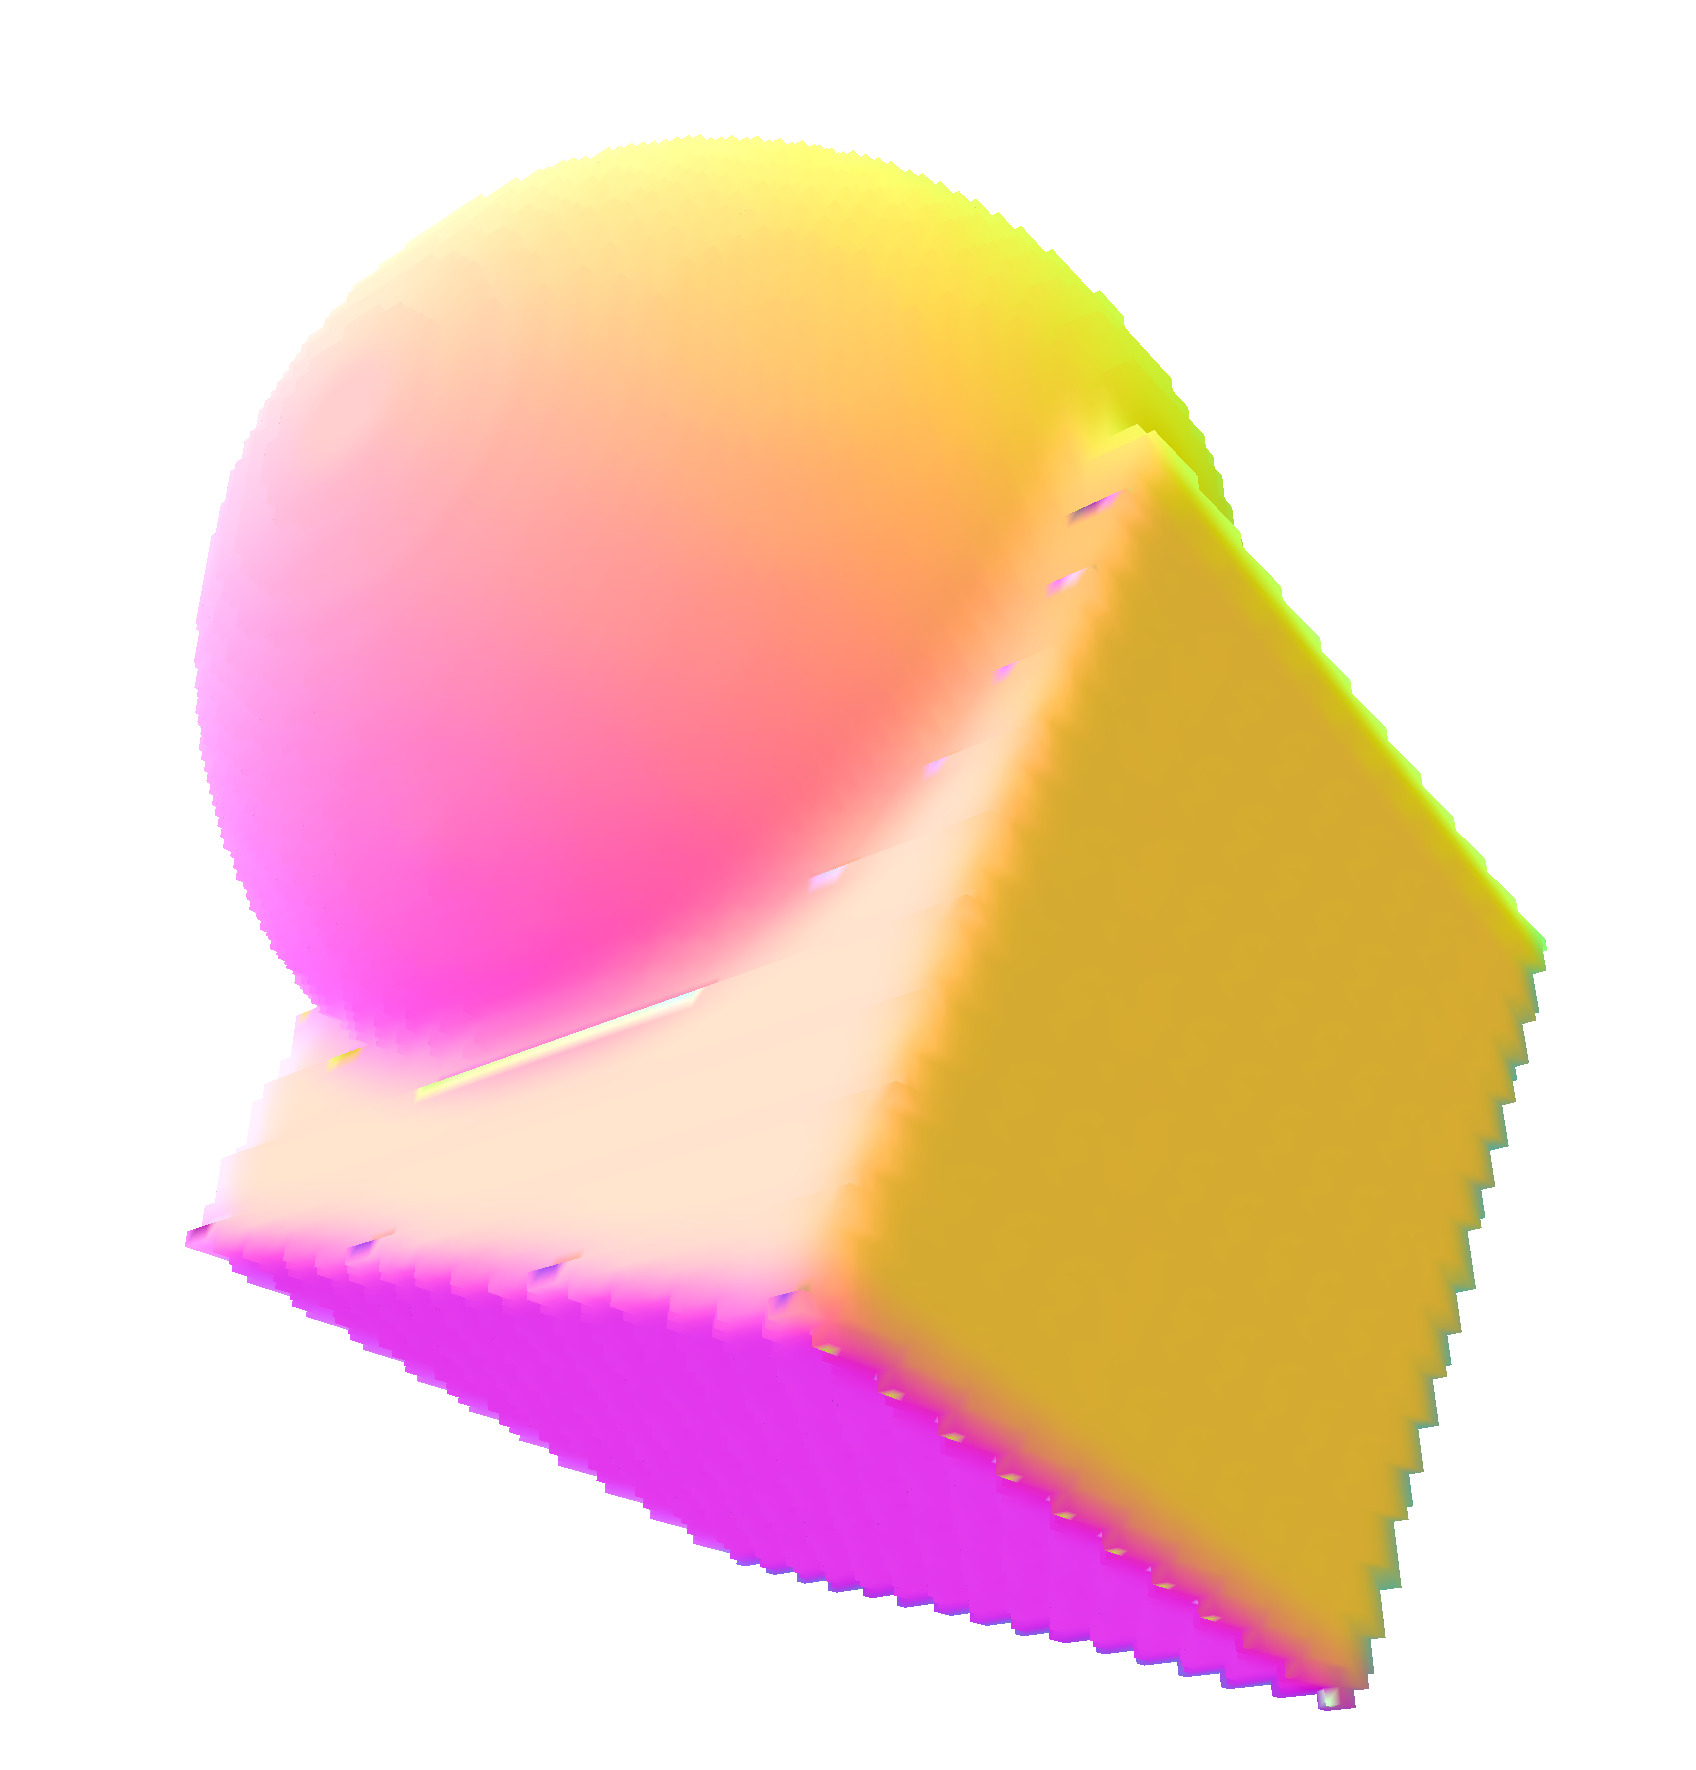
\includegraphics[width=0.3\textwidth]{pictures/cps-IIN-flat} \\
            %% 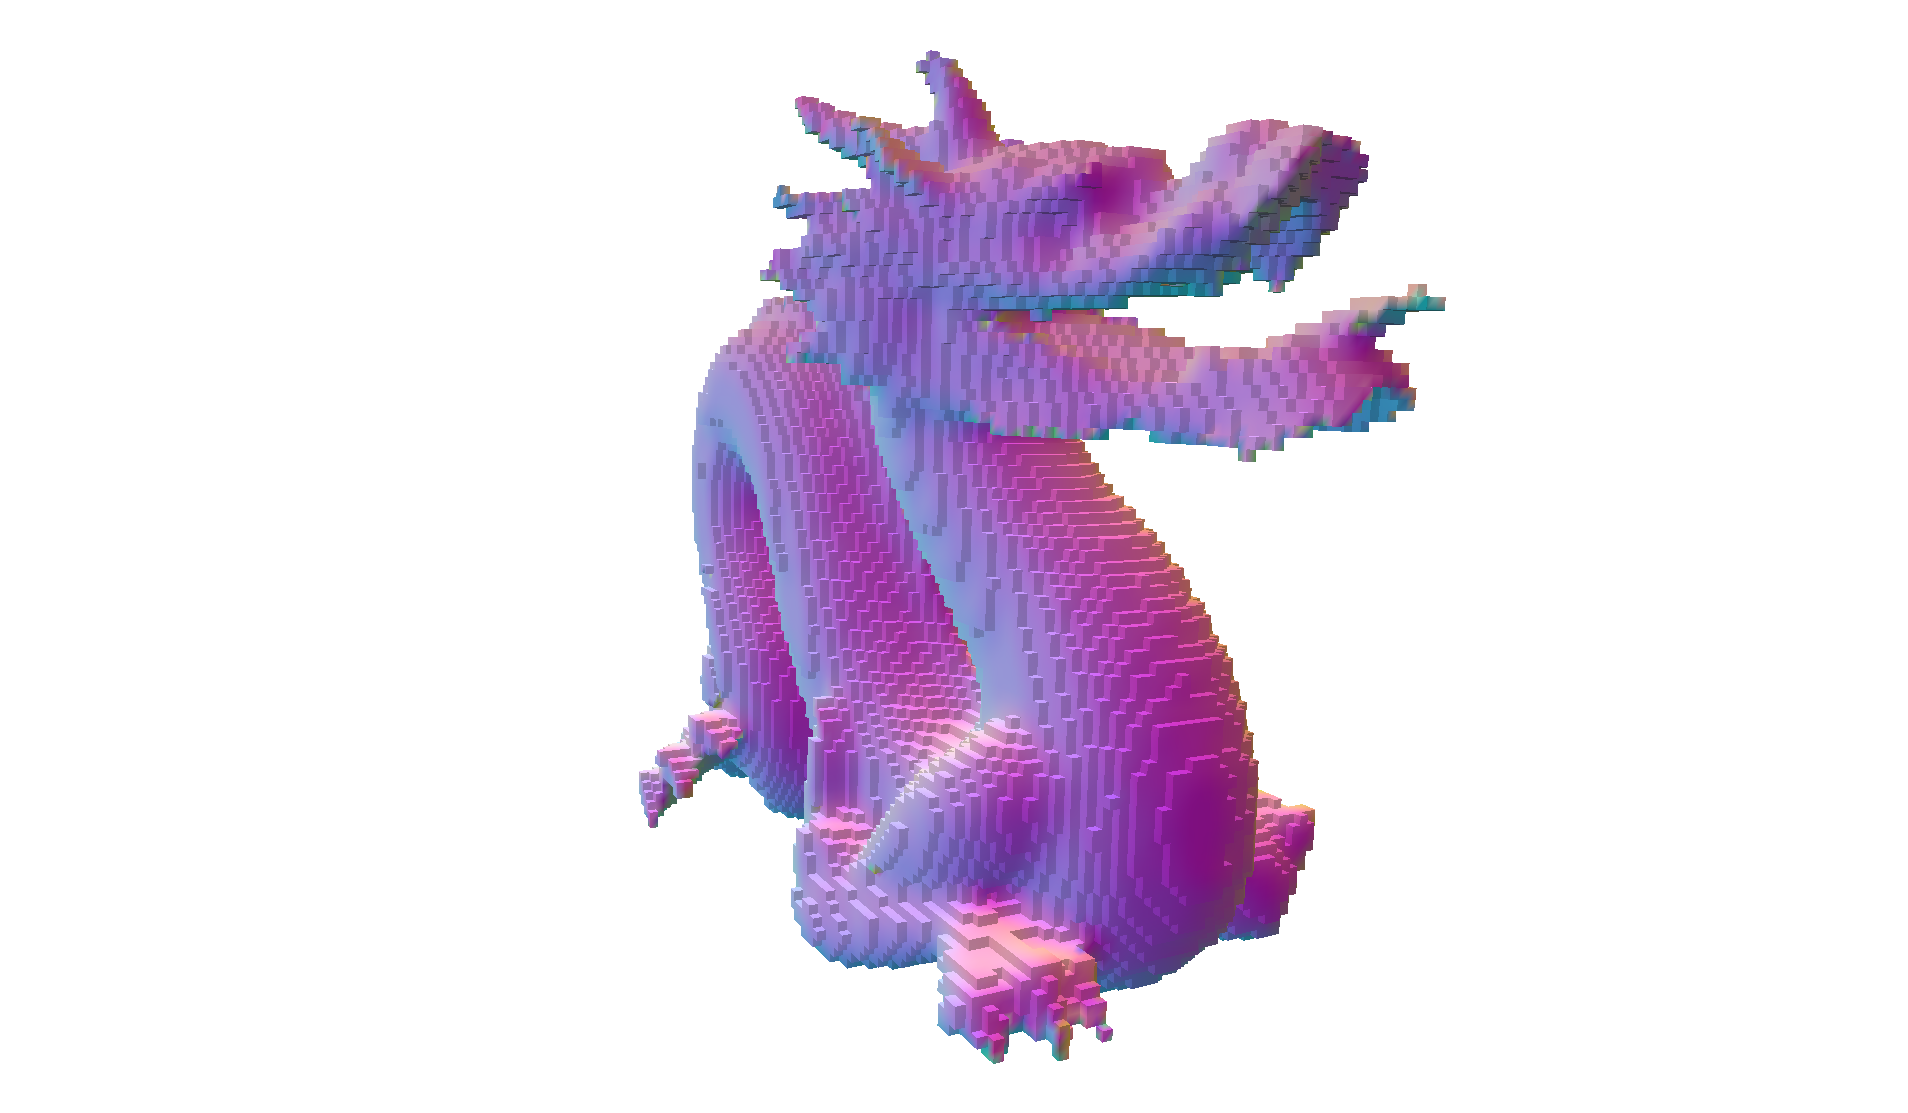
\includegraphics[width=0.4\textwidth]{pictures/chinese-dragon-normal-estimation-cubes-II} &
            %% 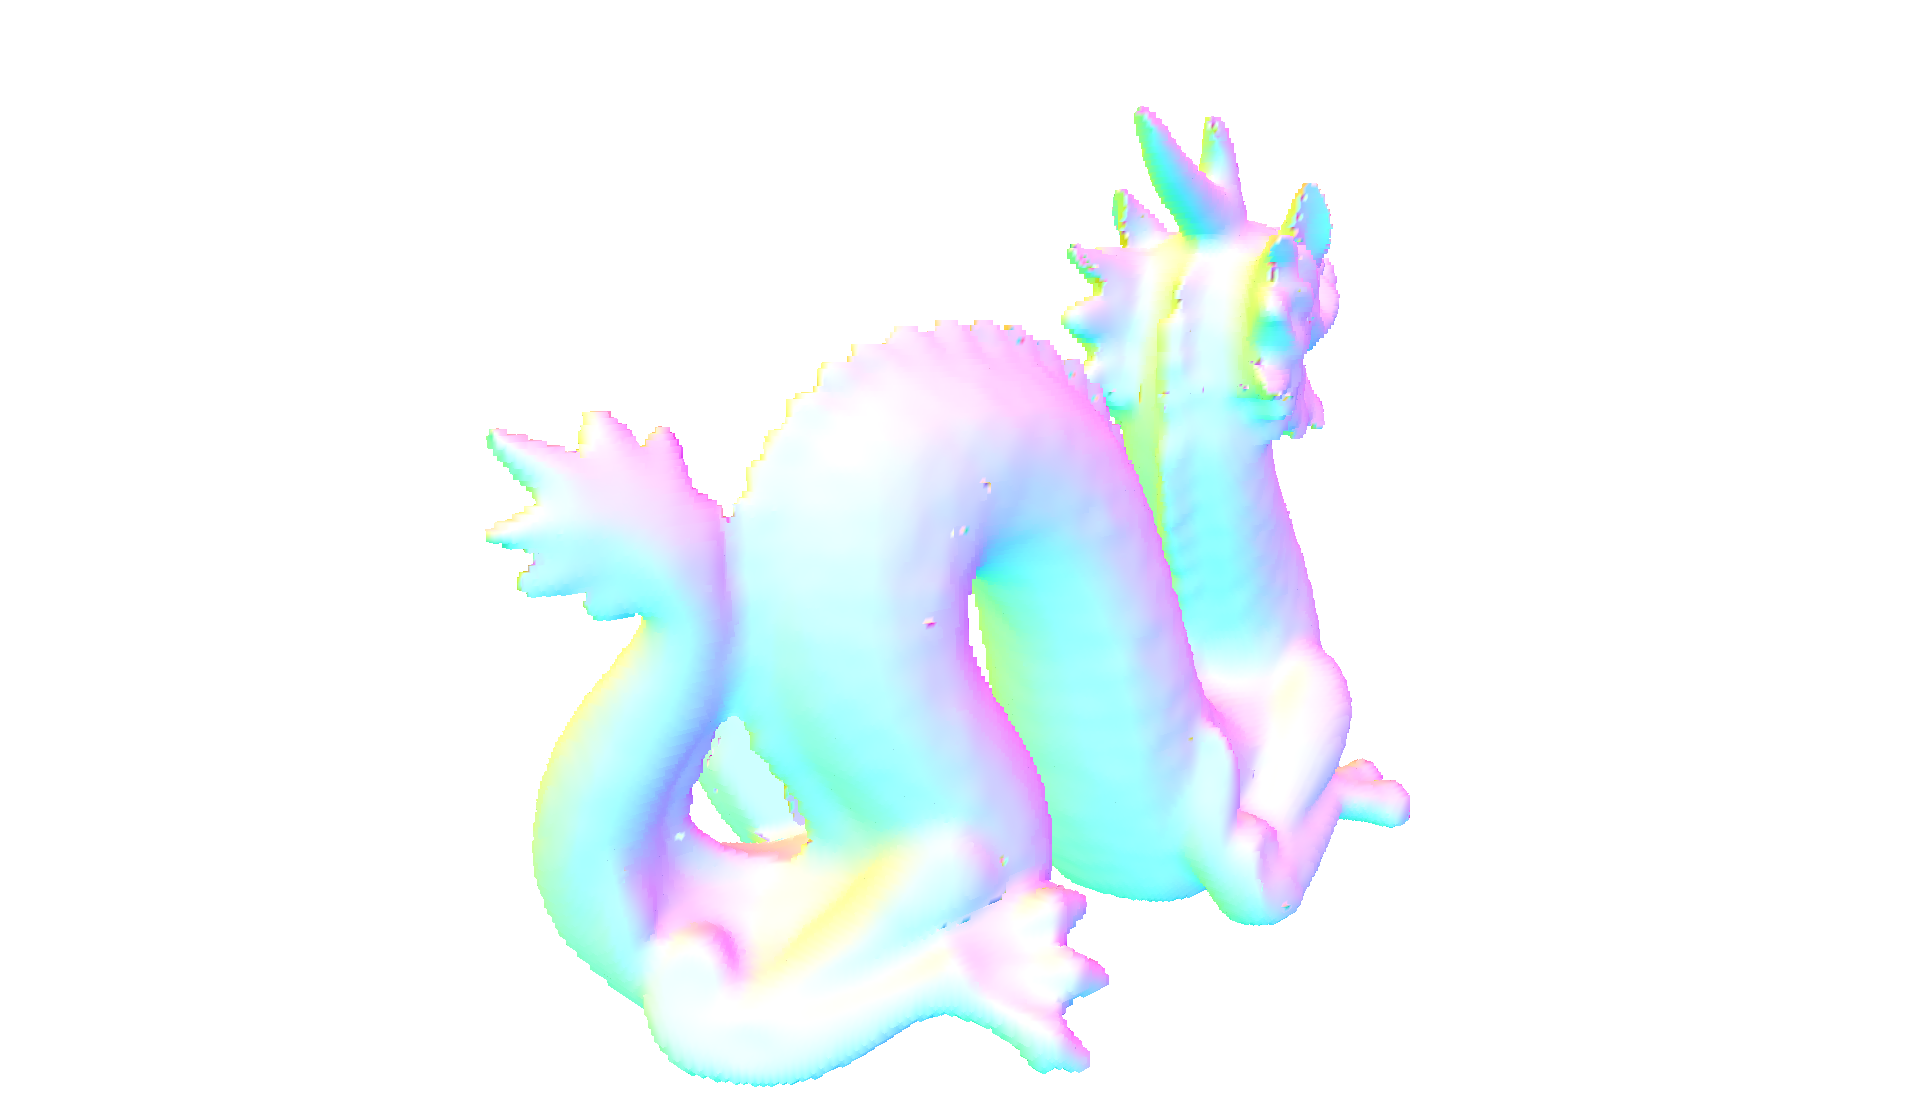
\includegraphics[width=0.4\textwidth]{pictures/chinese-dragon-normal-estimation-smooth-II} \\
            \hline
            \raisebox{18mm}{Ours} &
            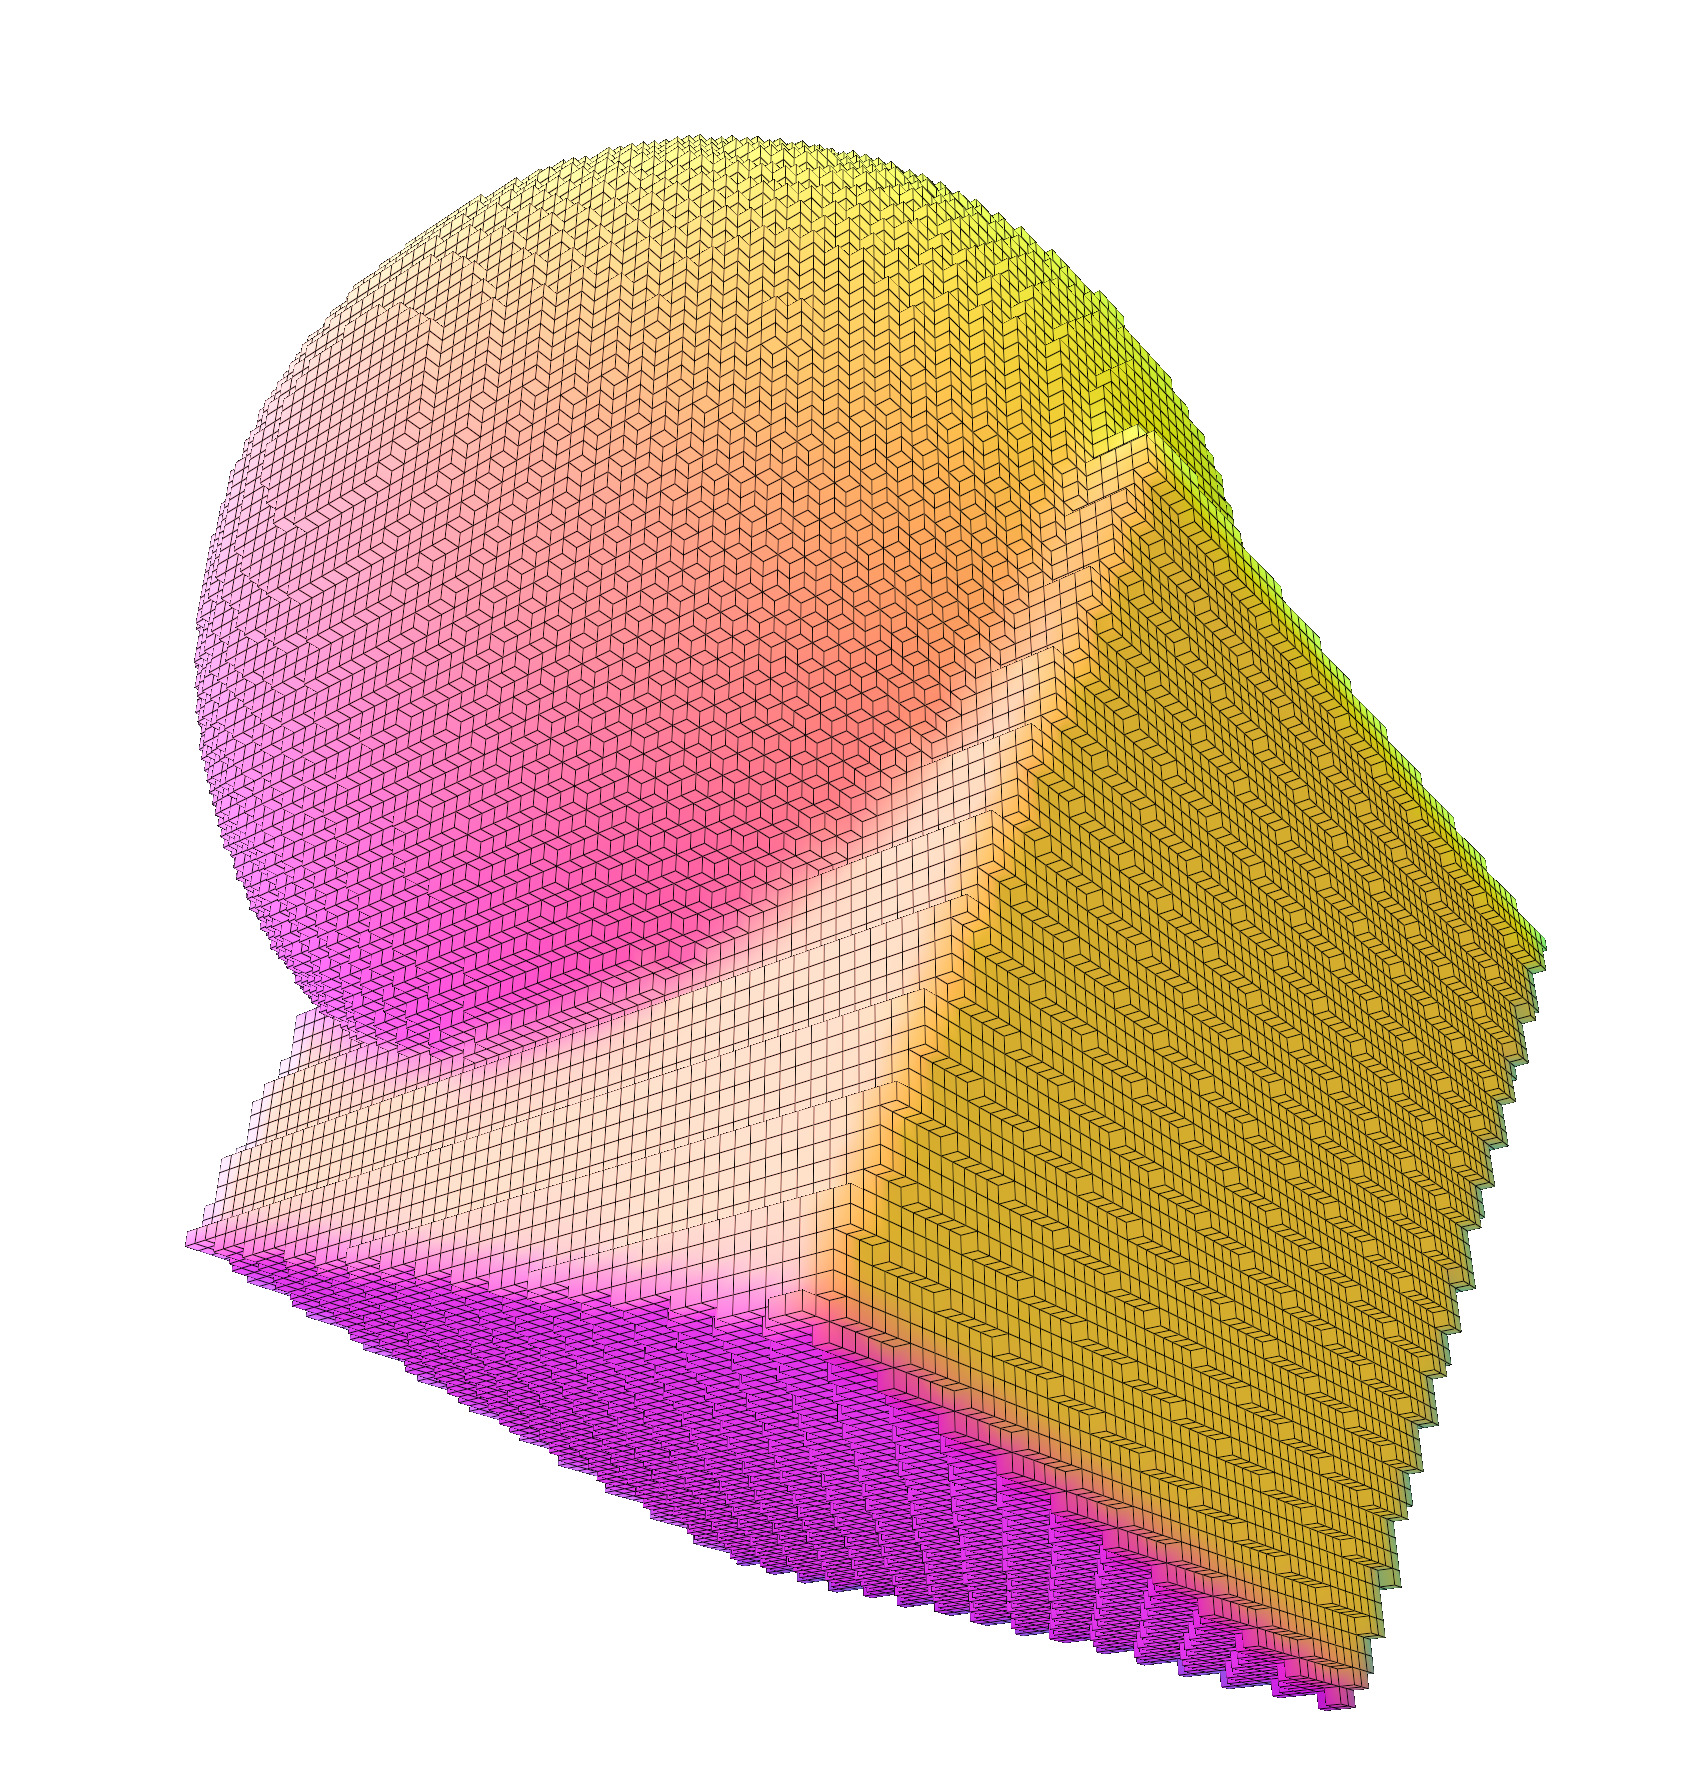
\includegraphics[width=0.3\textwidth]{pictures/cps-VN-flat-edge} &
            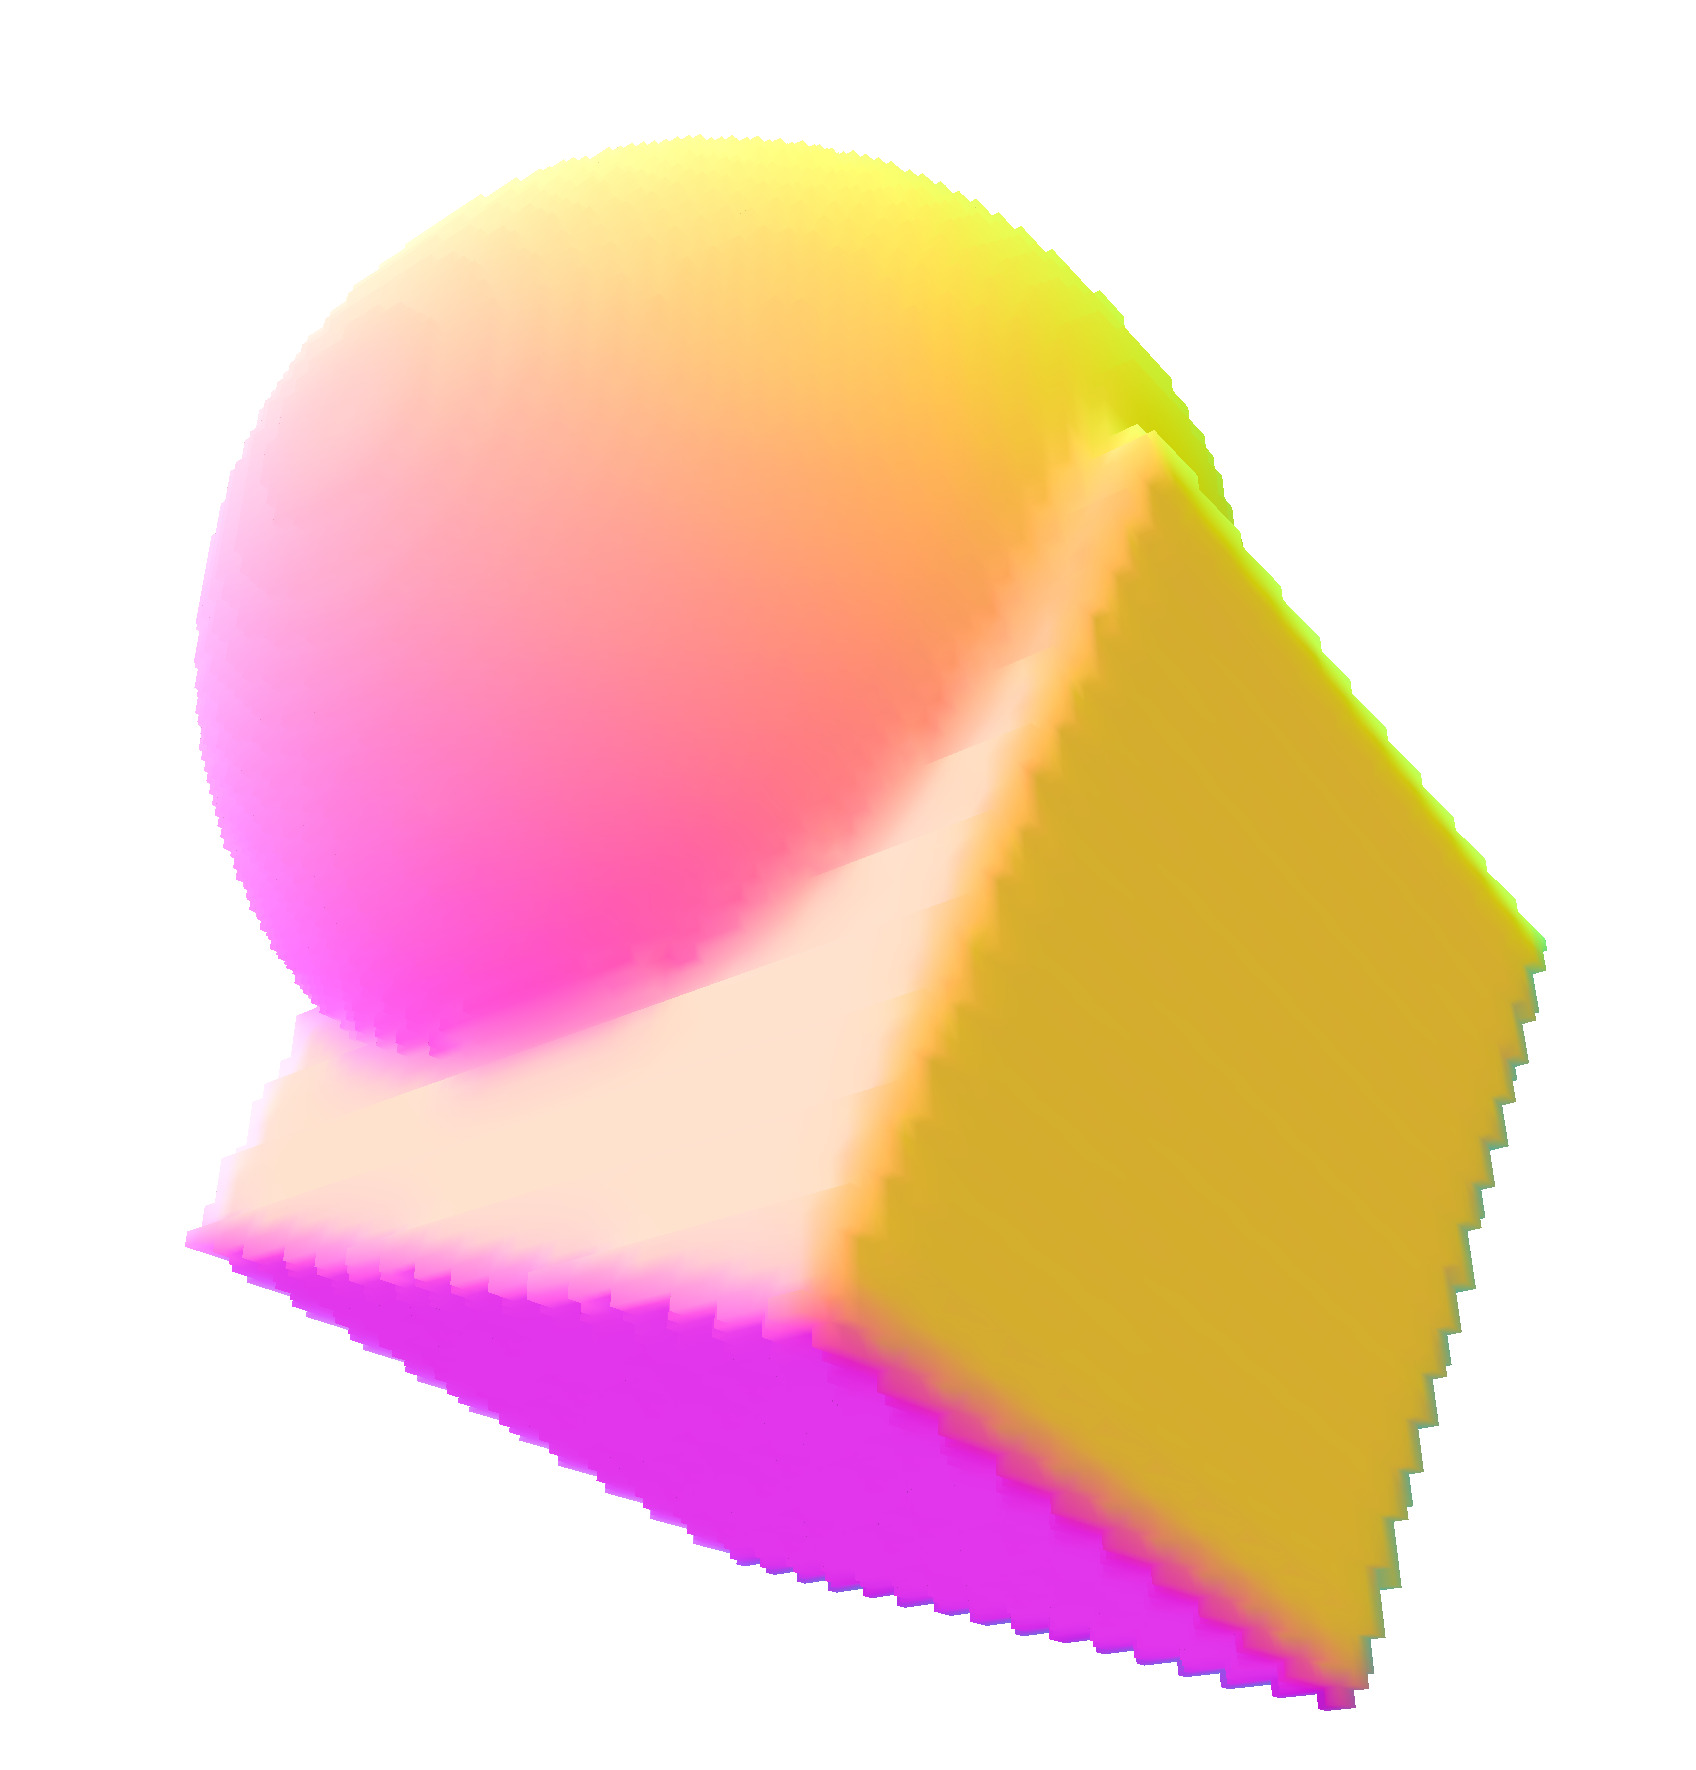
\includegraphics[width=0.3\textwidth]{pictures/cps-VN-flat} \\
            %% 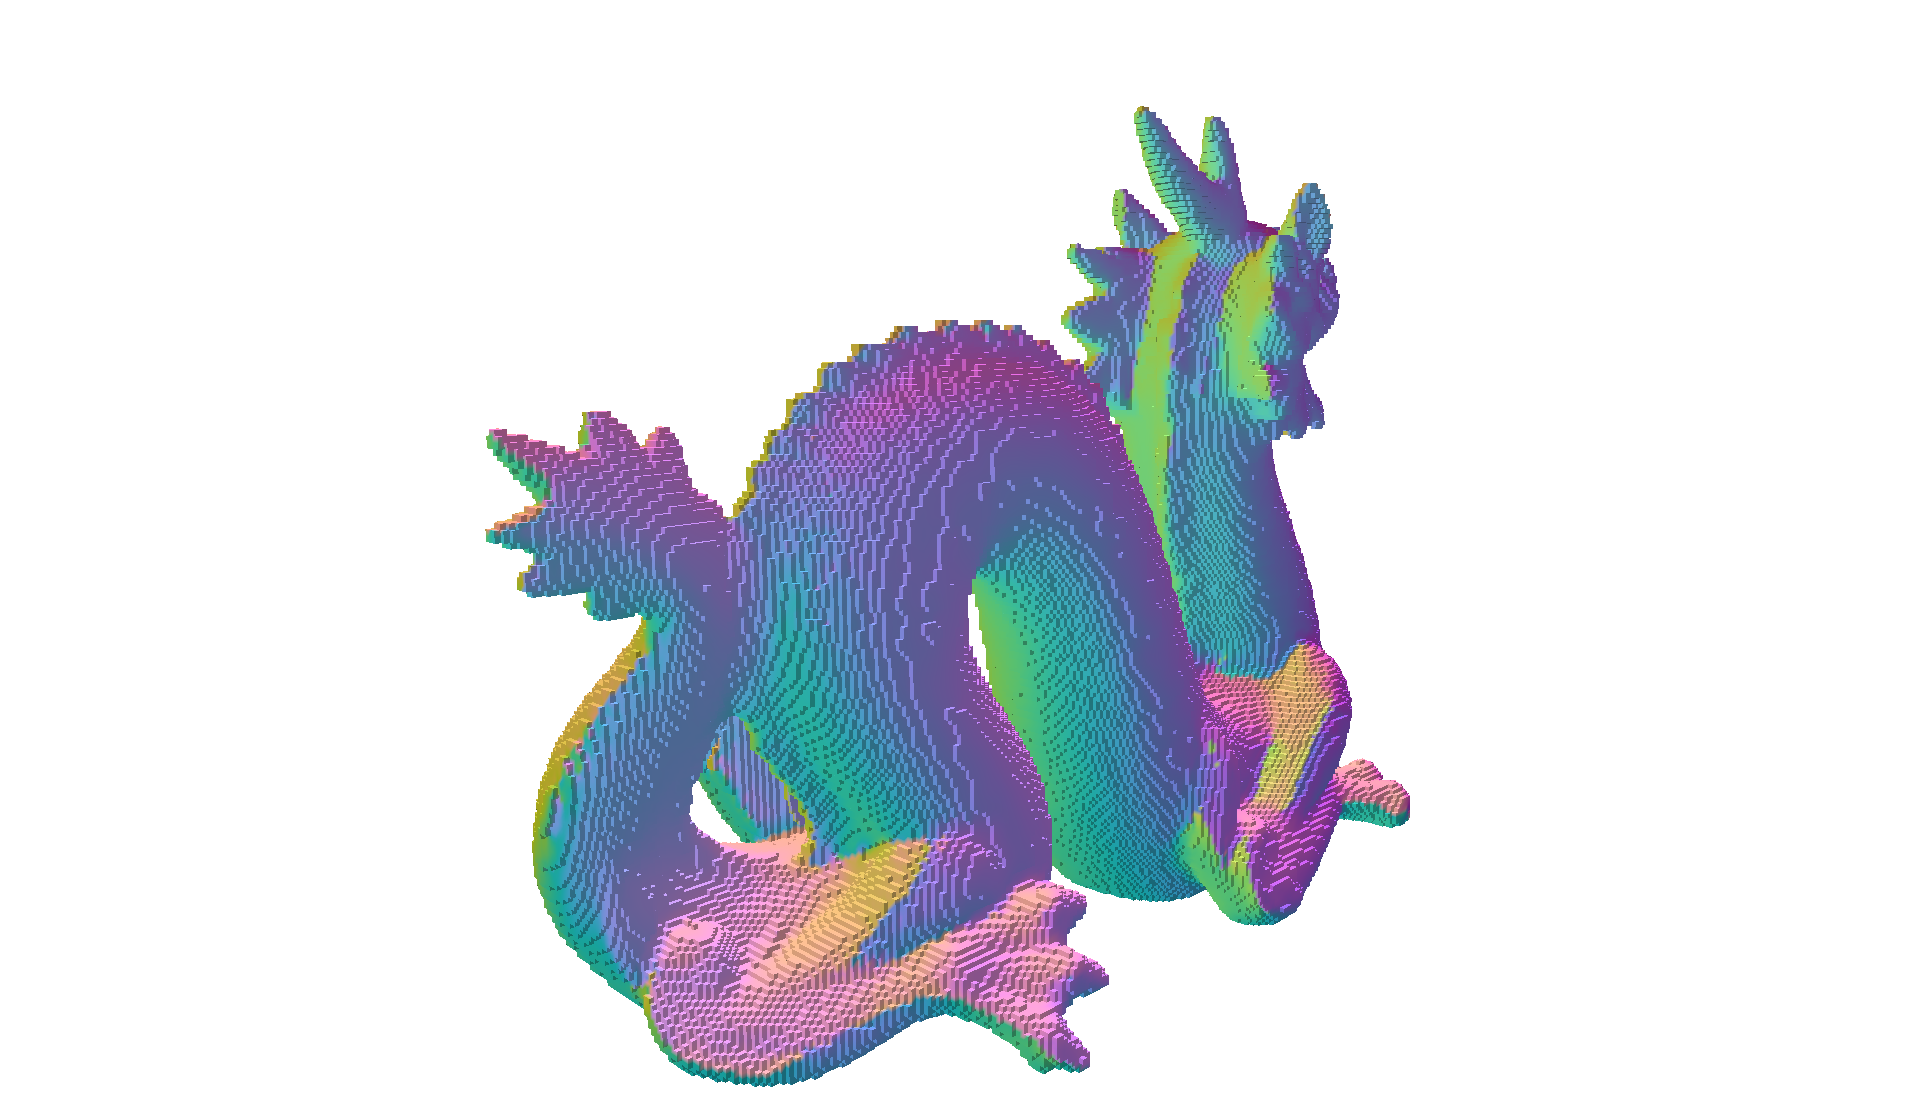
\includegraphics[width=0.4\textwidth]{pictures/chinese-dragon-normal-estimation-cubes-NV} &
            %% 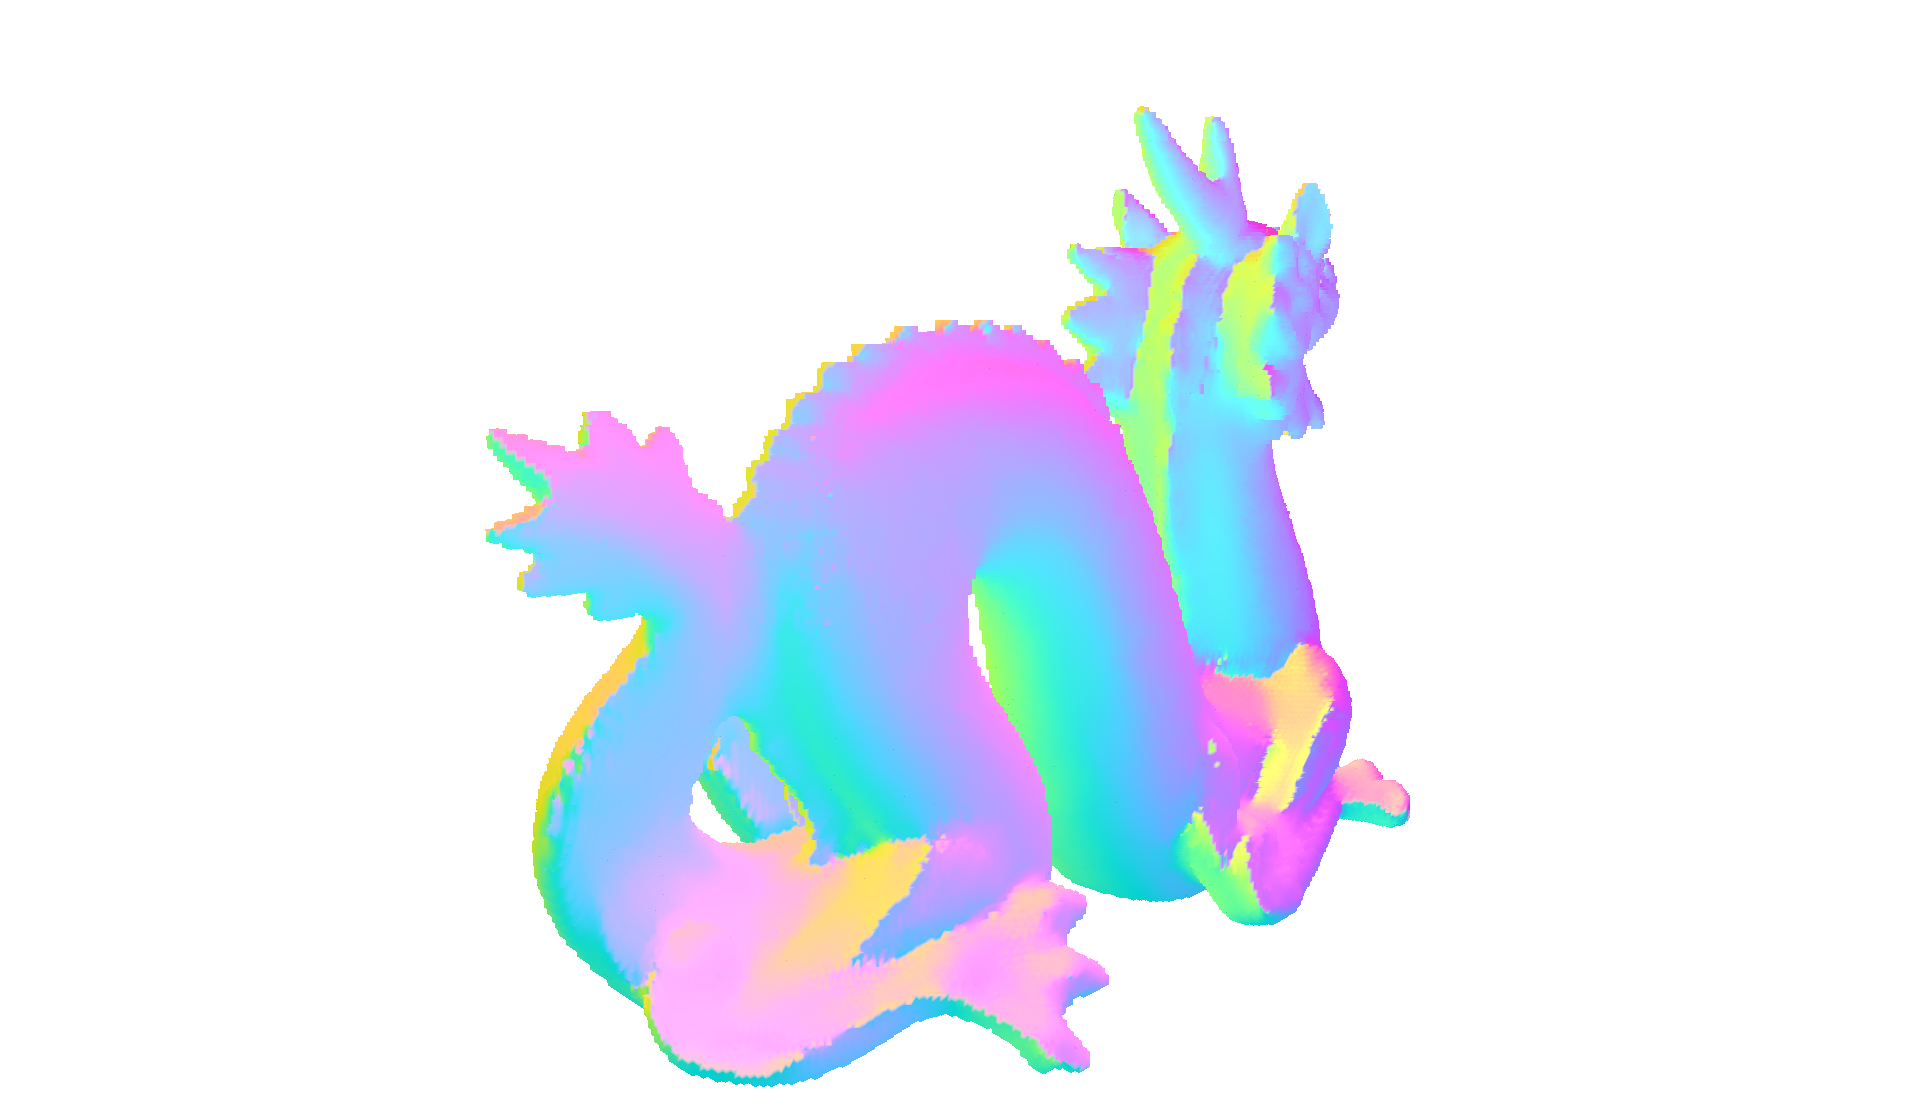
\includegraphics[width=0.4\textwidth]{pictures/chinese-dragon-normal-estimation-smooth-NV} \\
            \hline
            \raisebox{18mm}{II} &
            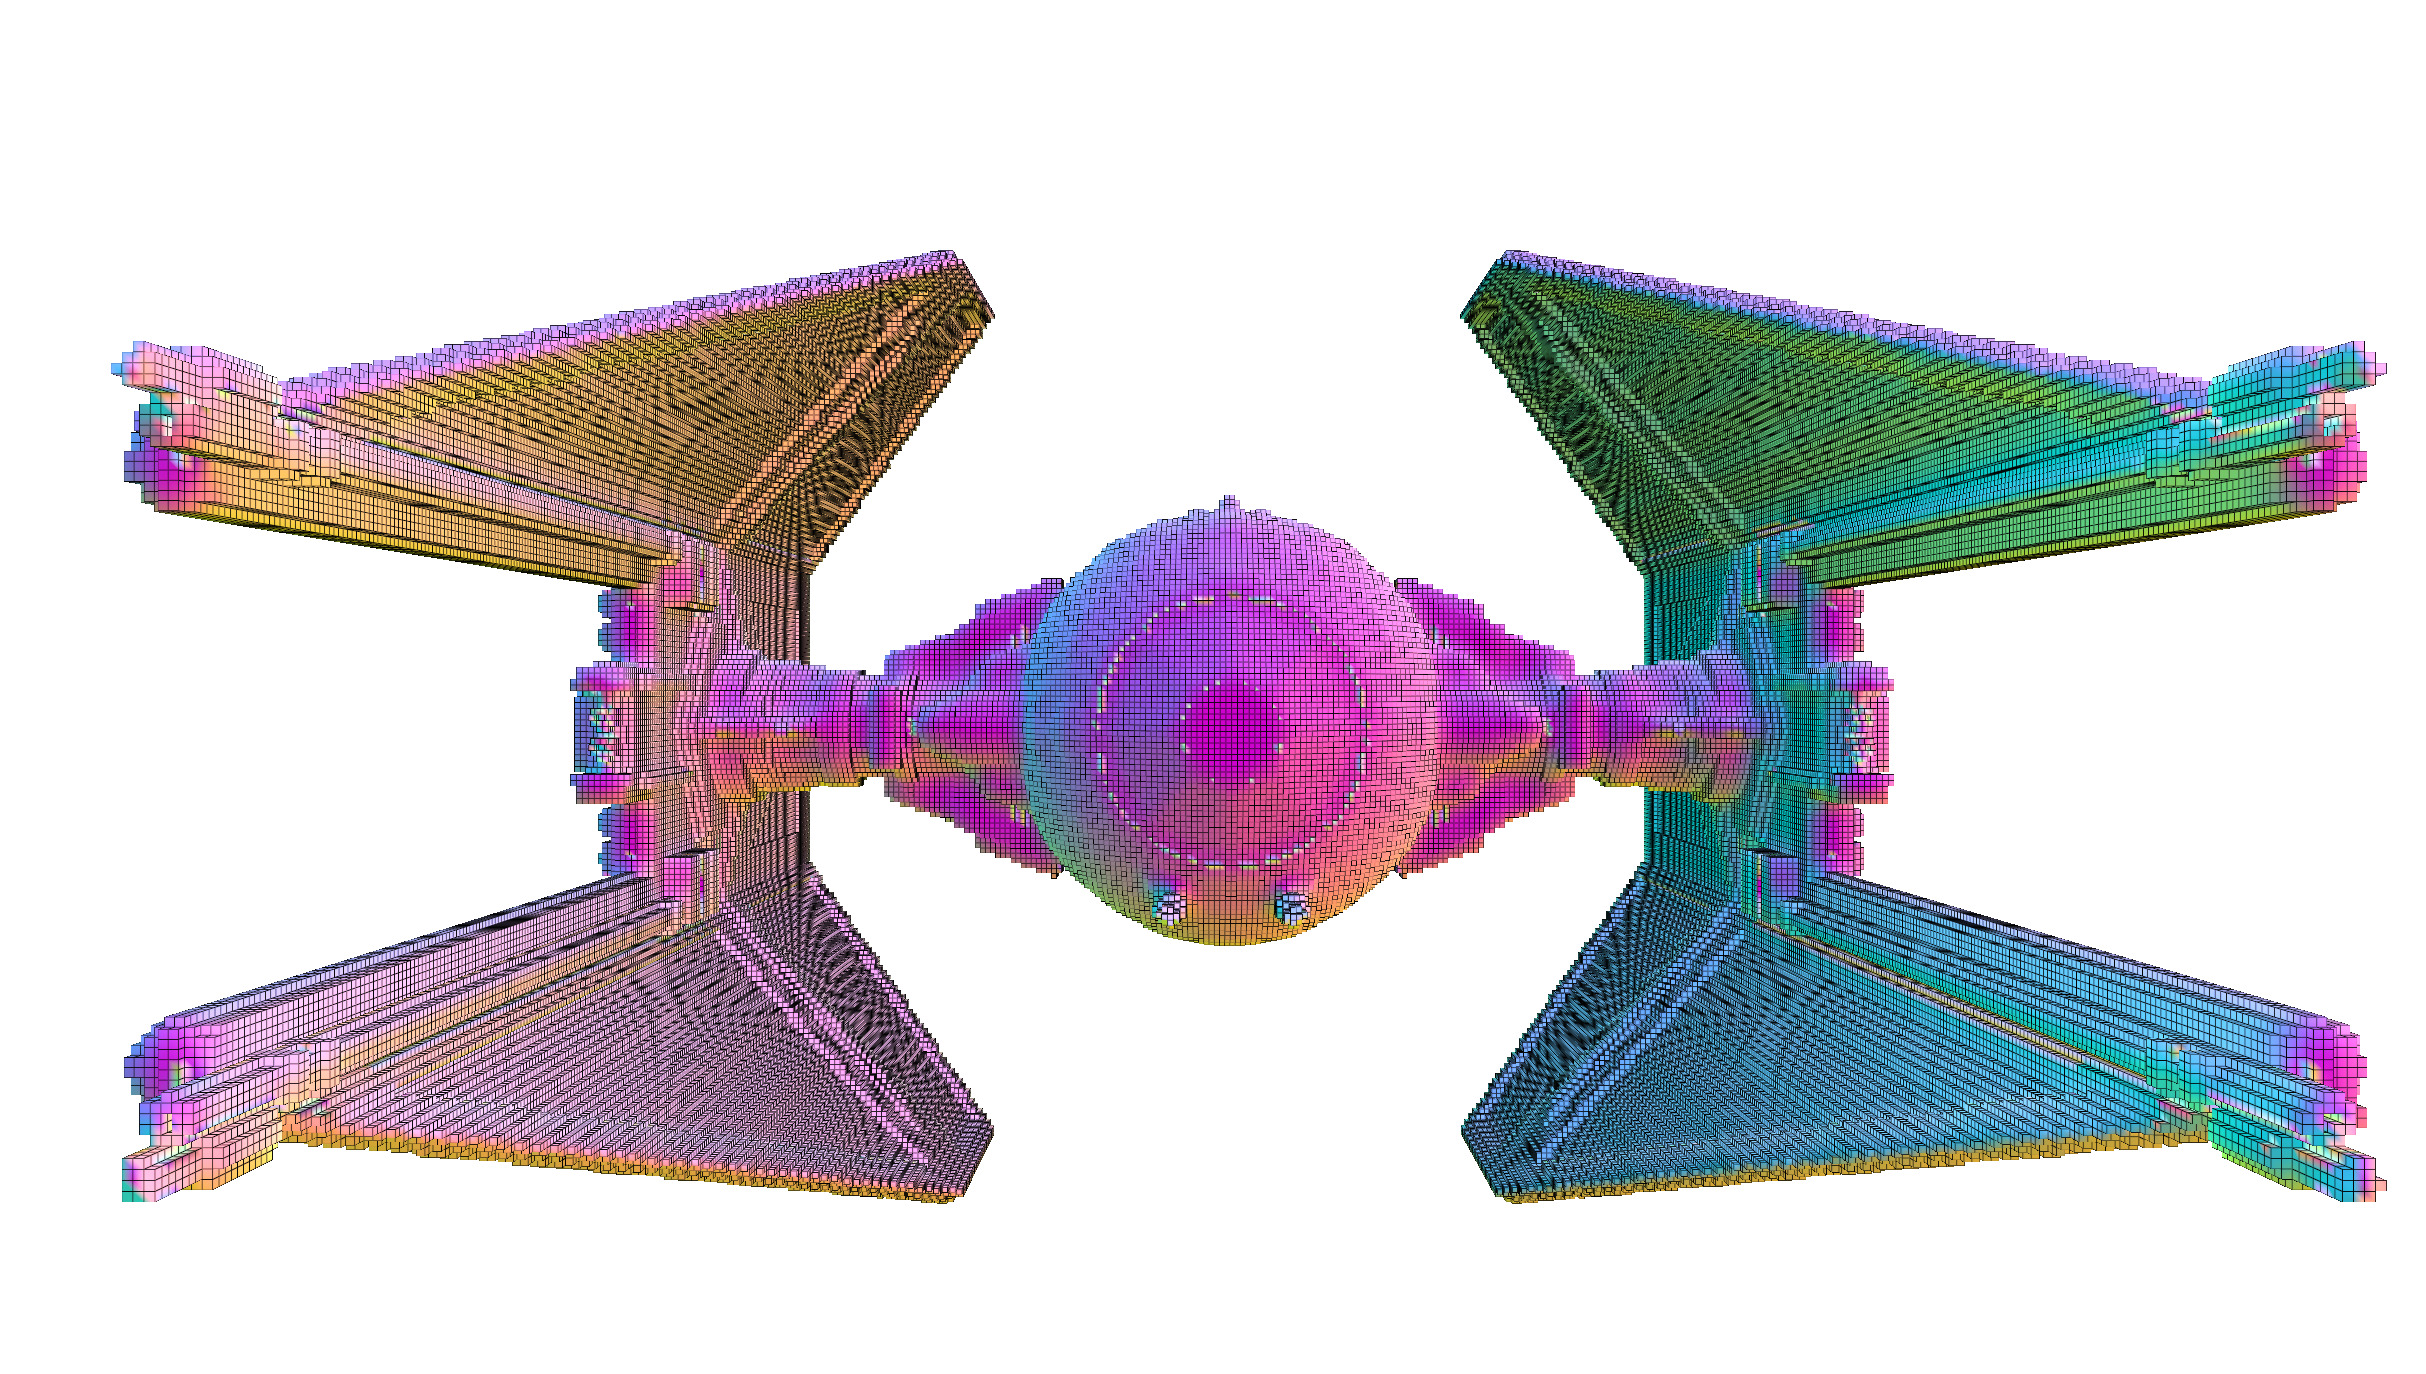
\includegraphics[width=0.43\textwidth]{pictures/tie256-IIN-flat-edge} &
            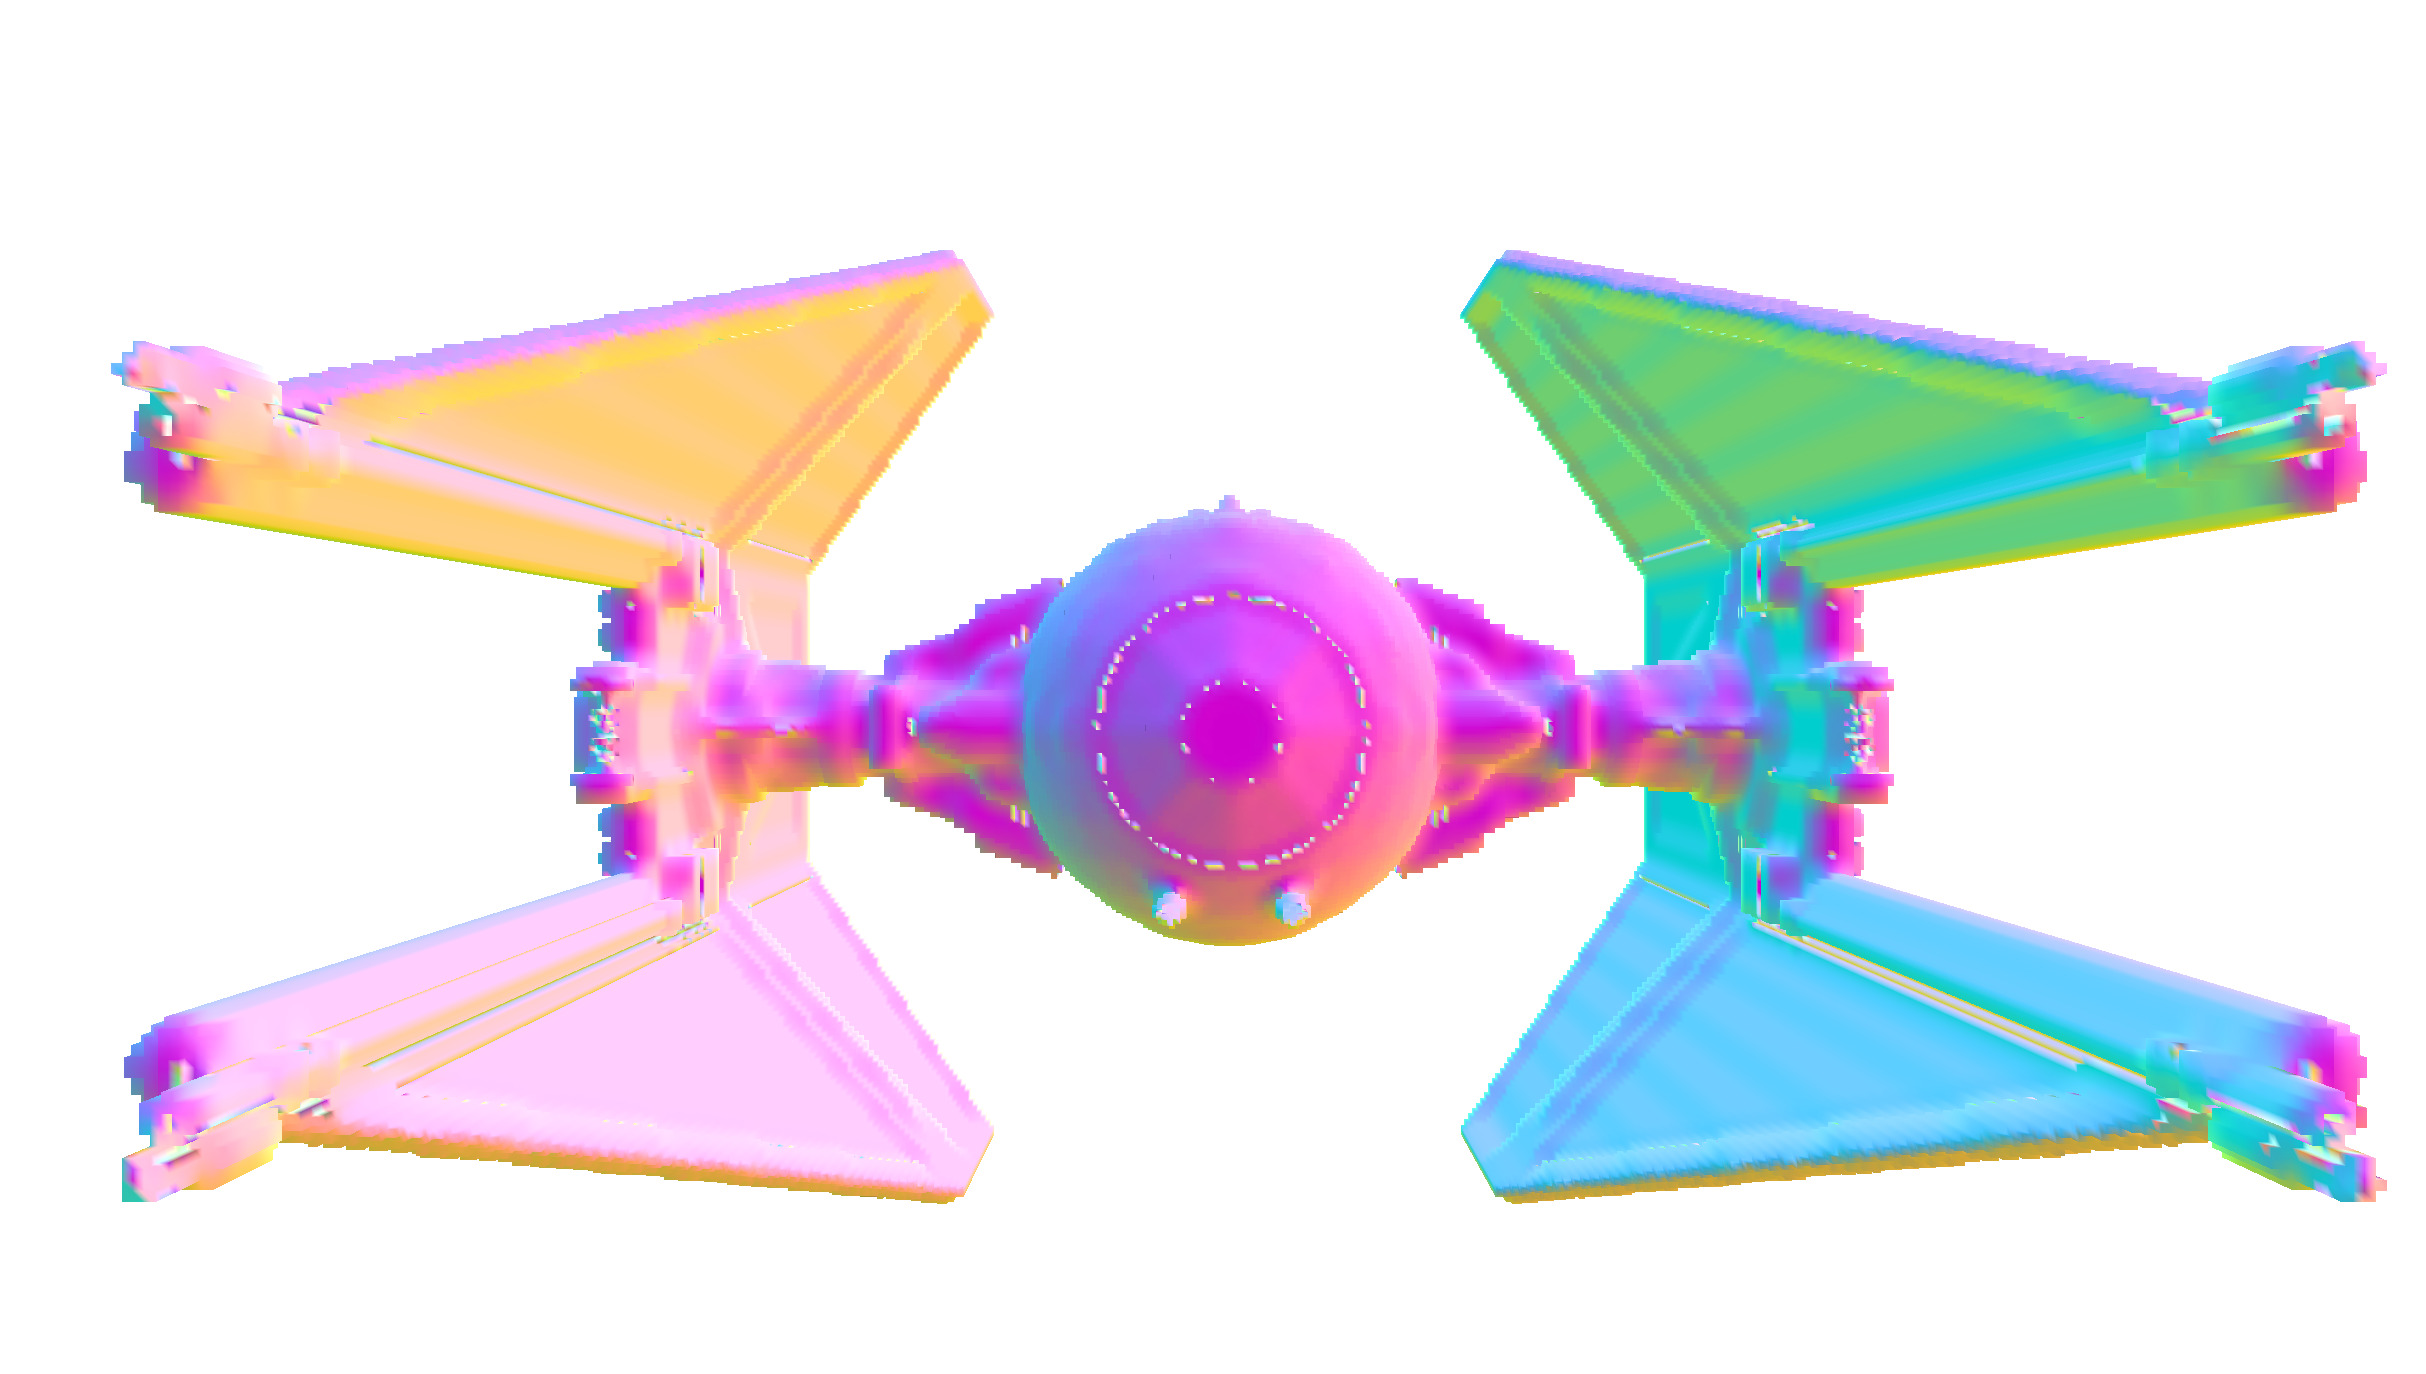
\includegraphics[width=0.43\textwidth]{pictures/tie256-IIN-flat} \\
            %% 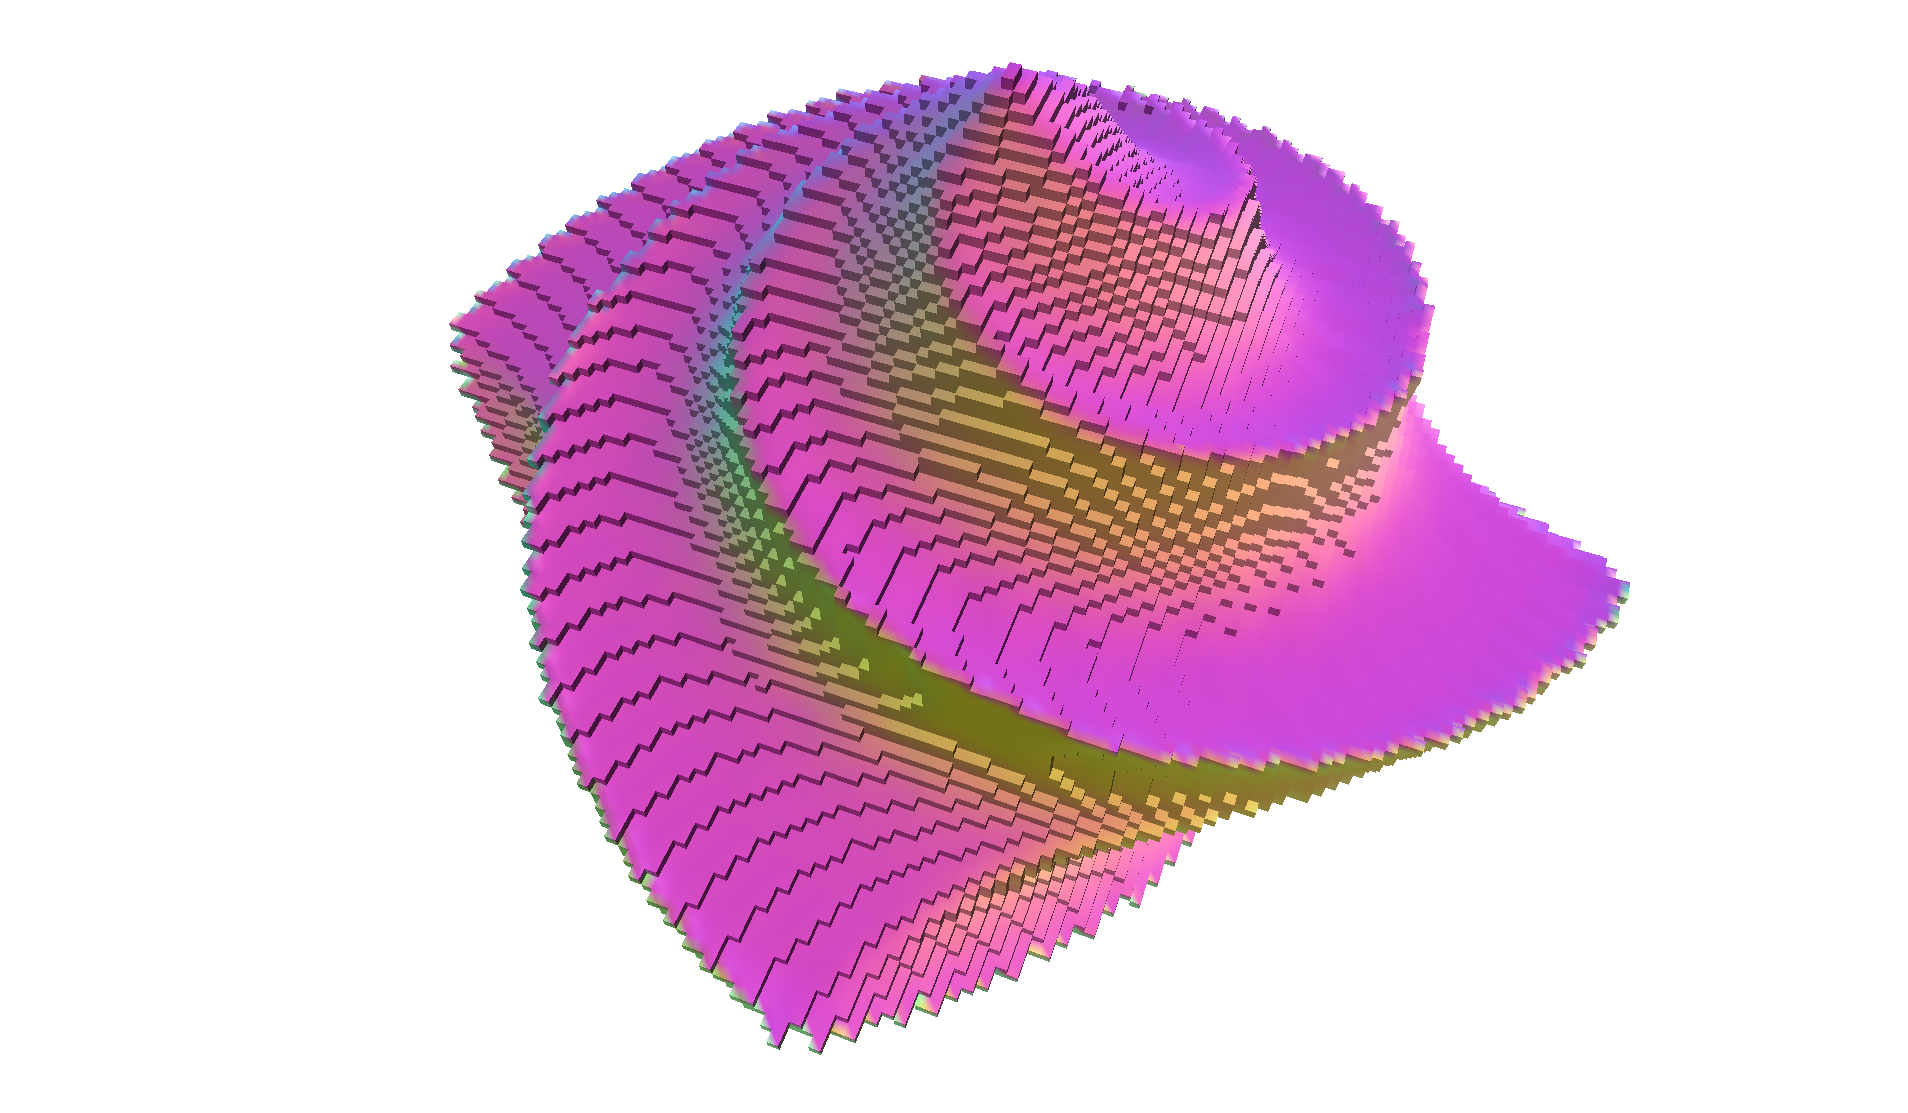
\includegraphics[width=0.4\textwidth]{pictures/octaflower-normal-estimation-cubes-II} &
            %% 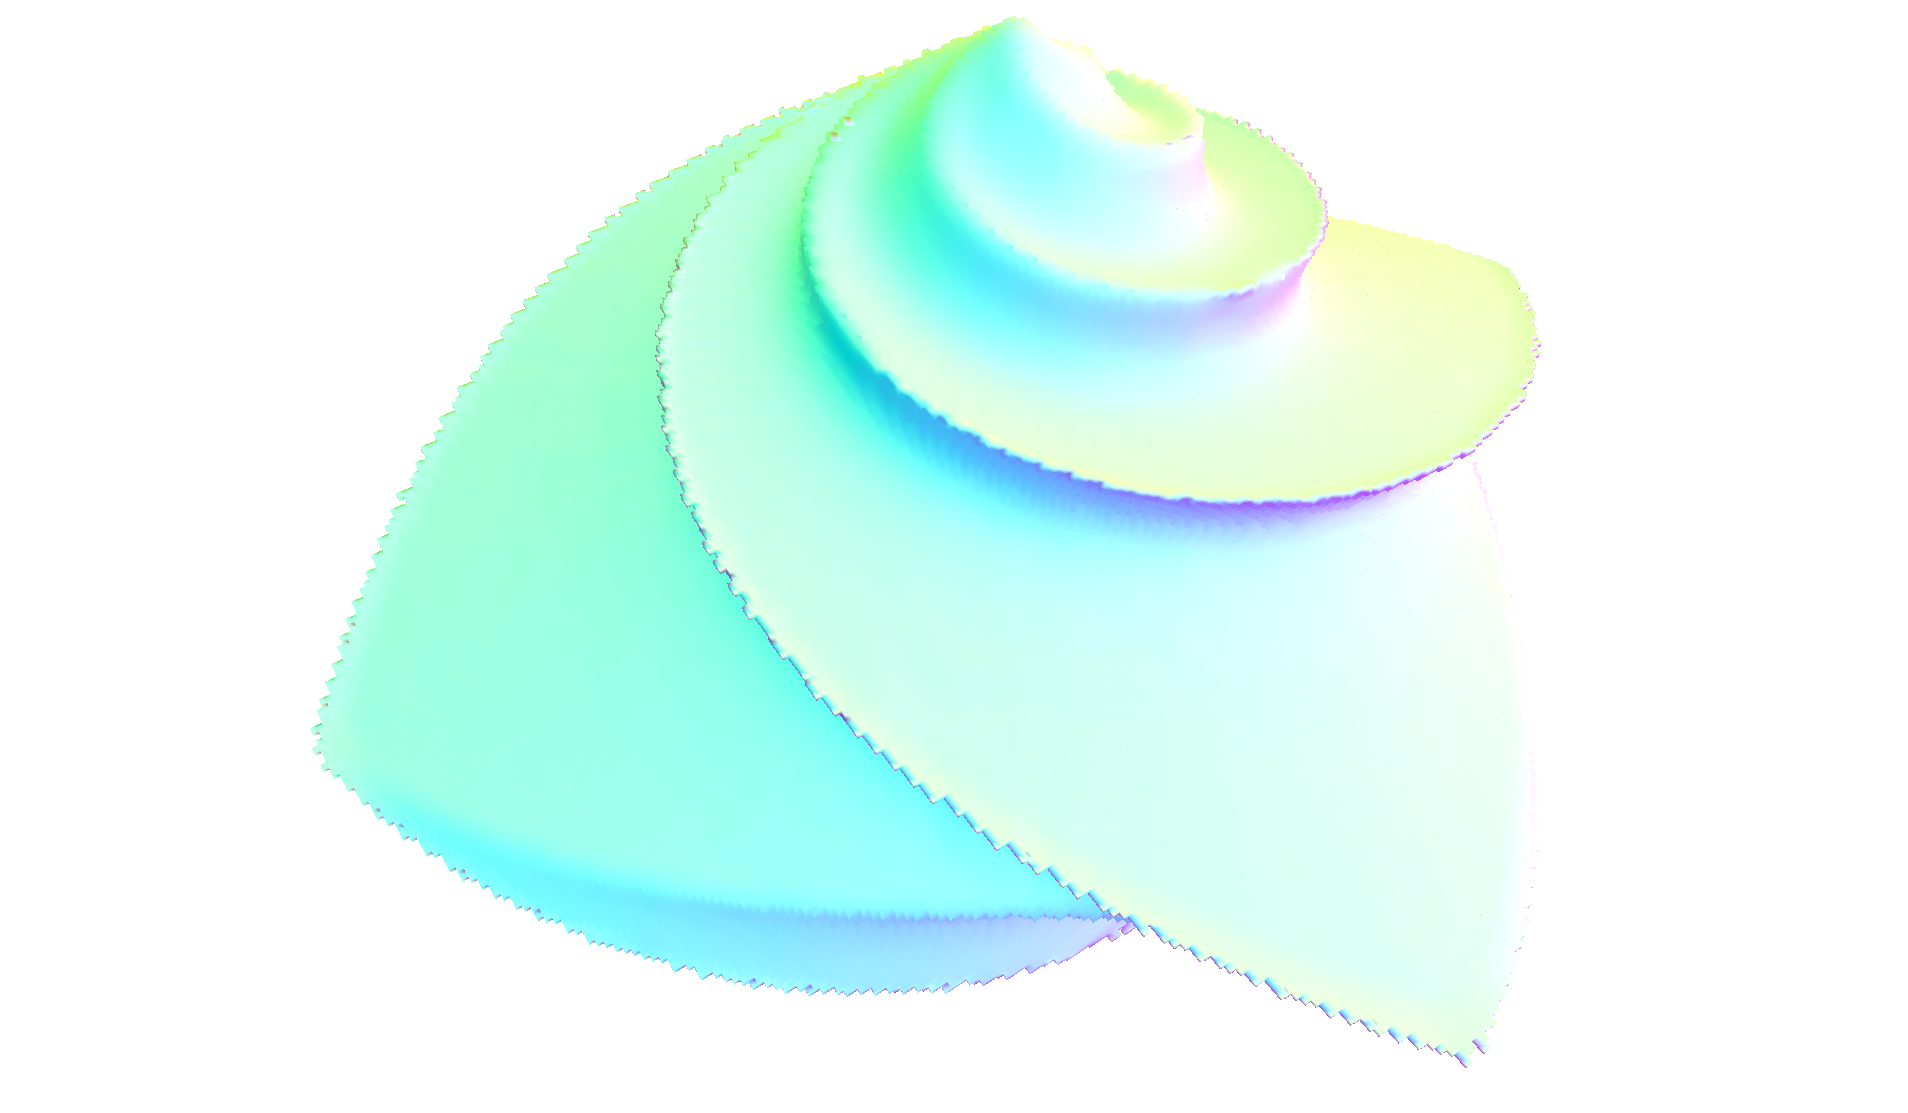
\includegraphics[width=0.4\textwidth]{pictures/octaflower-normal-estimation-smooth-II} \\
            \hline
            \raisebox{18mm}{Ours} &
            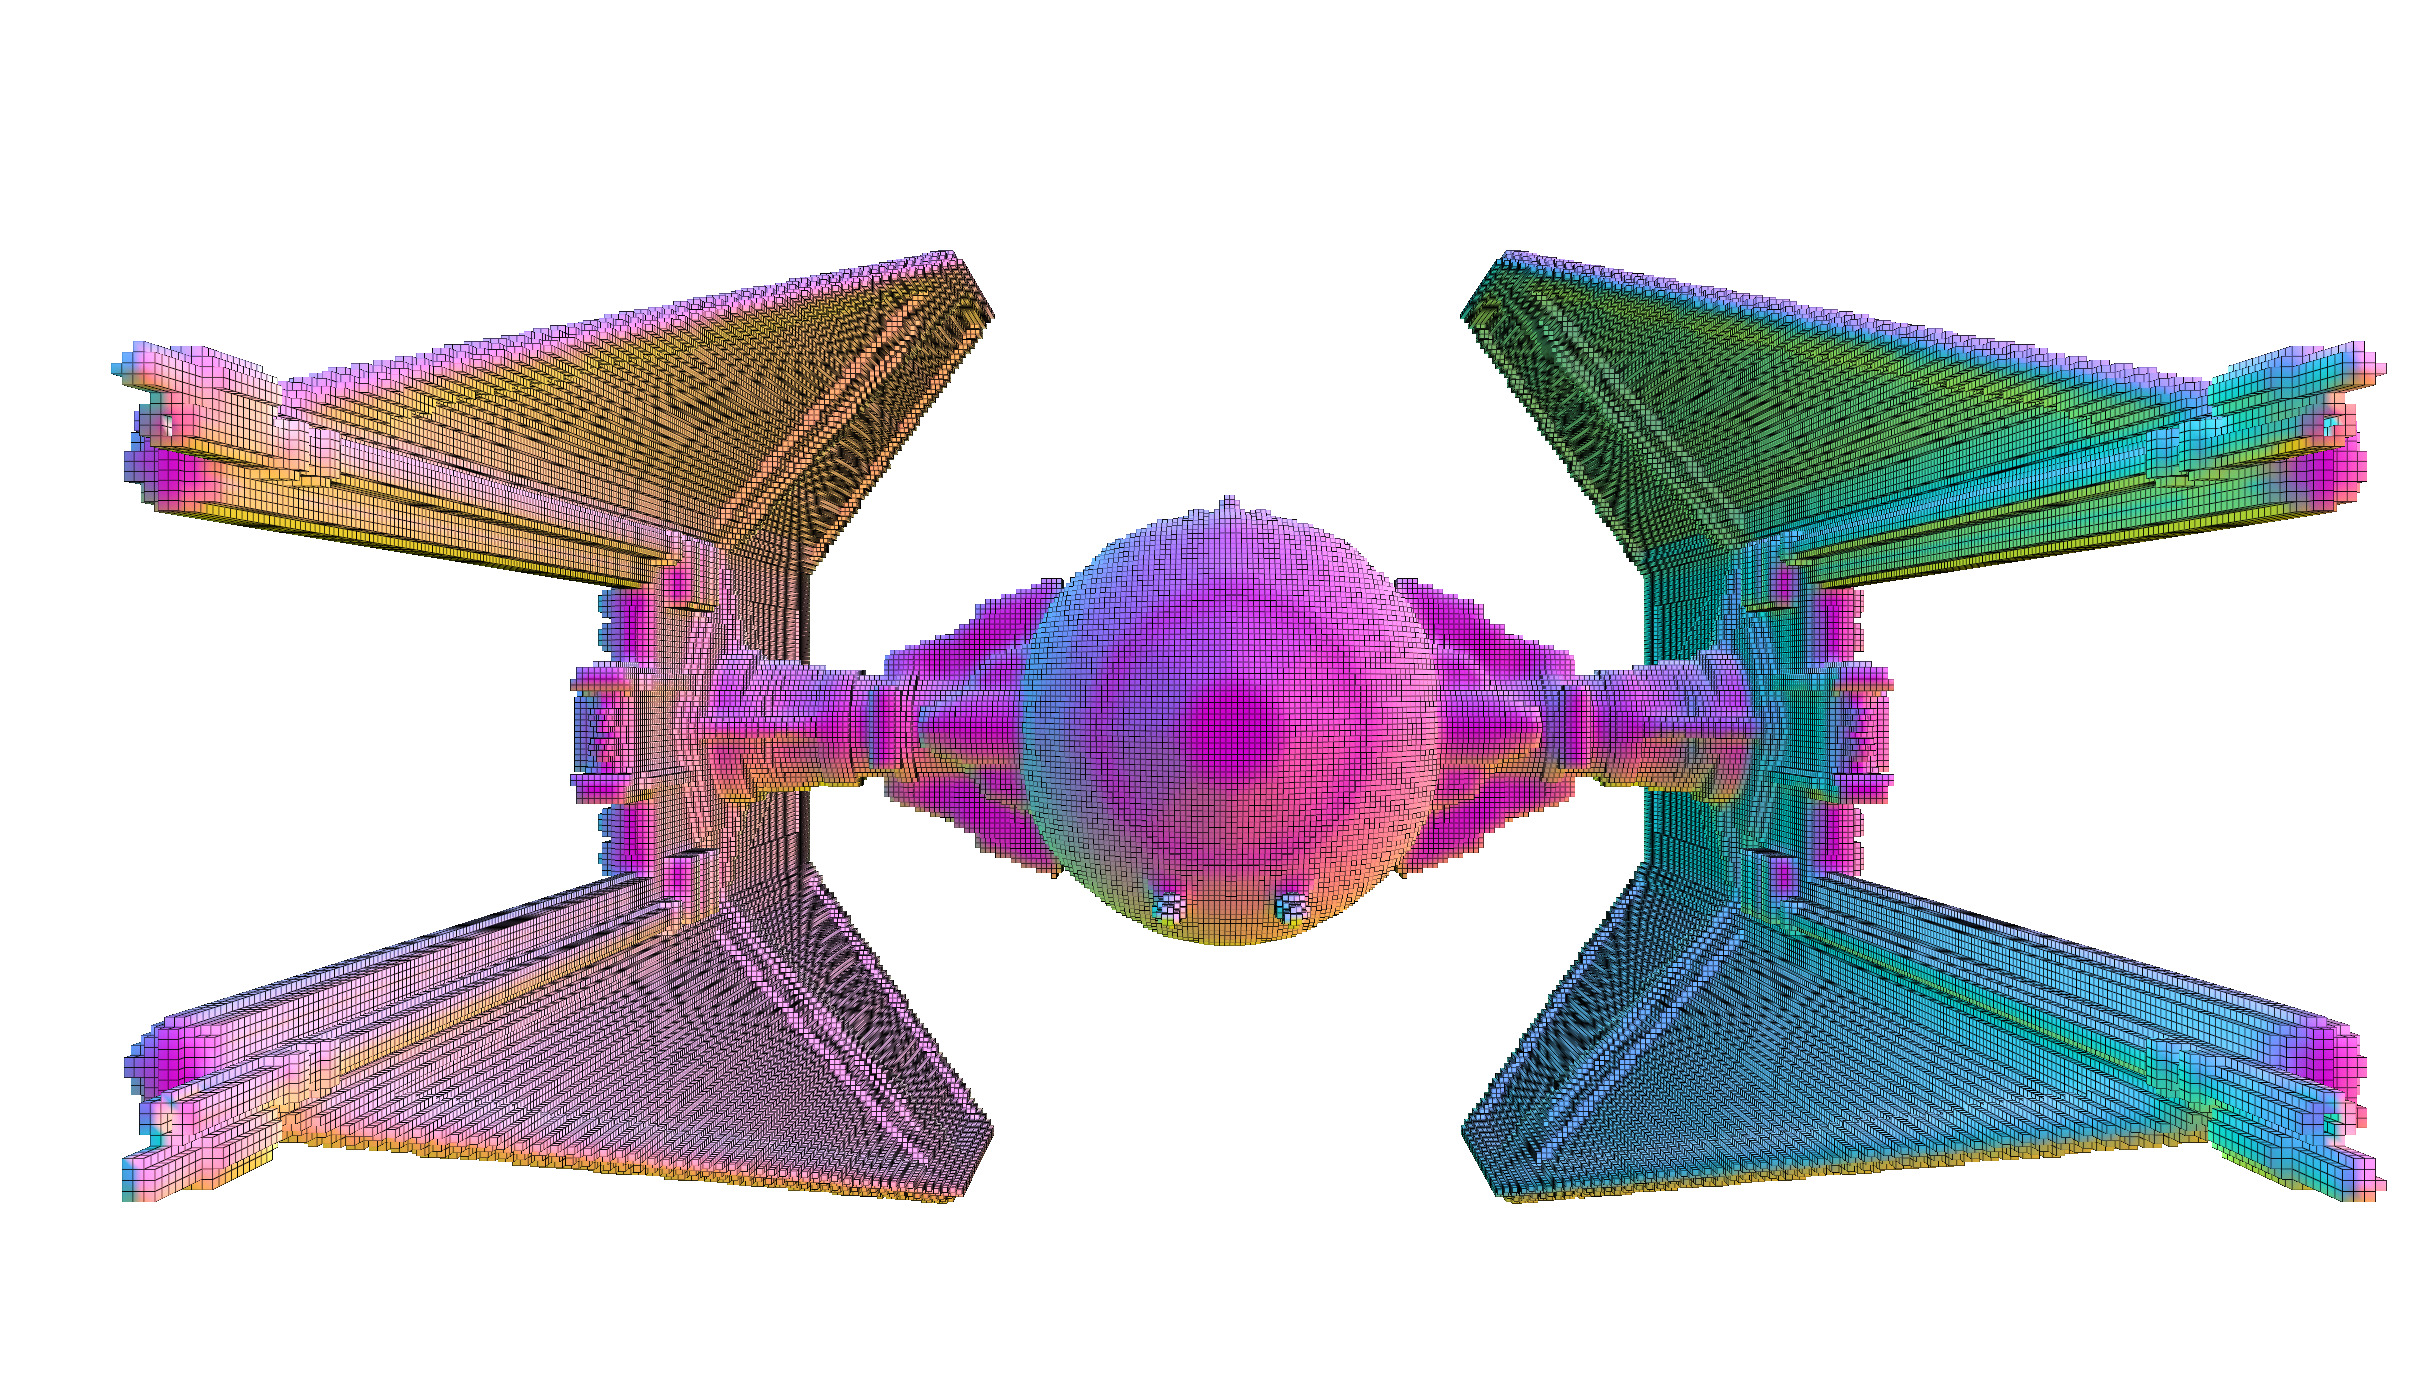
\includegraphics[width=0.43\textwidth]{pictures/tie256-VN-flat-edge} &
            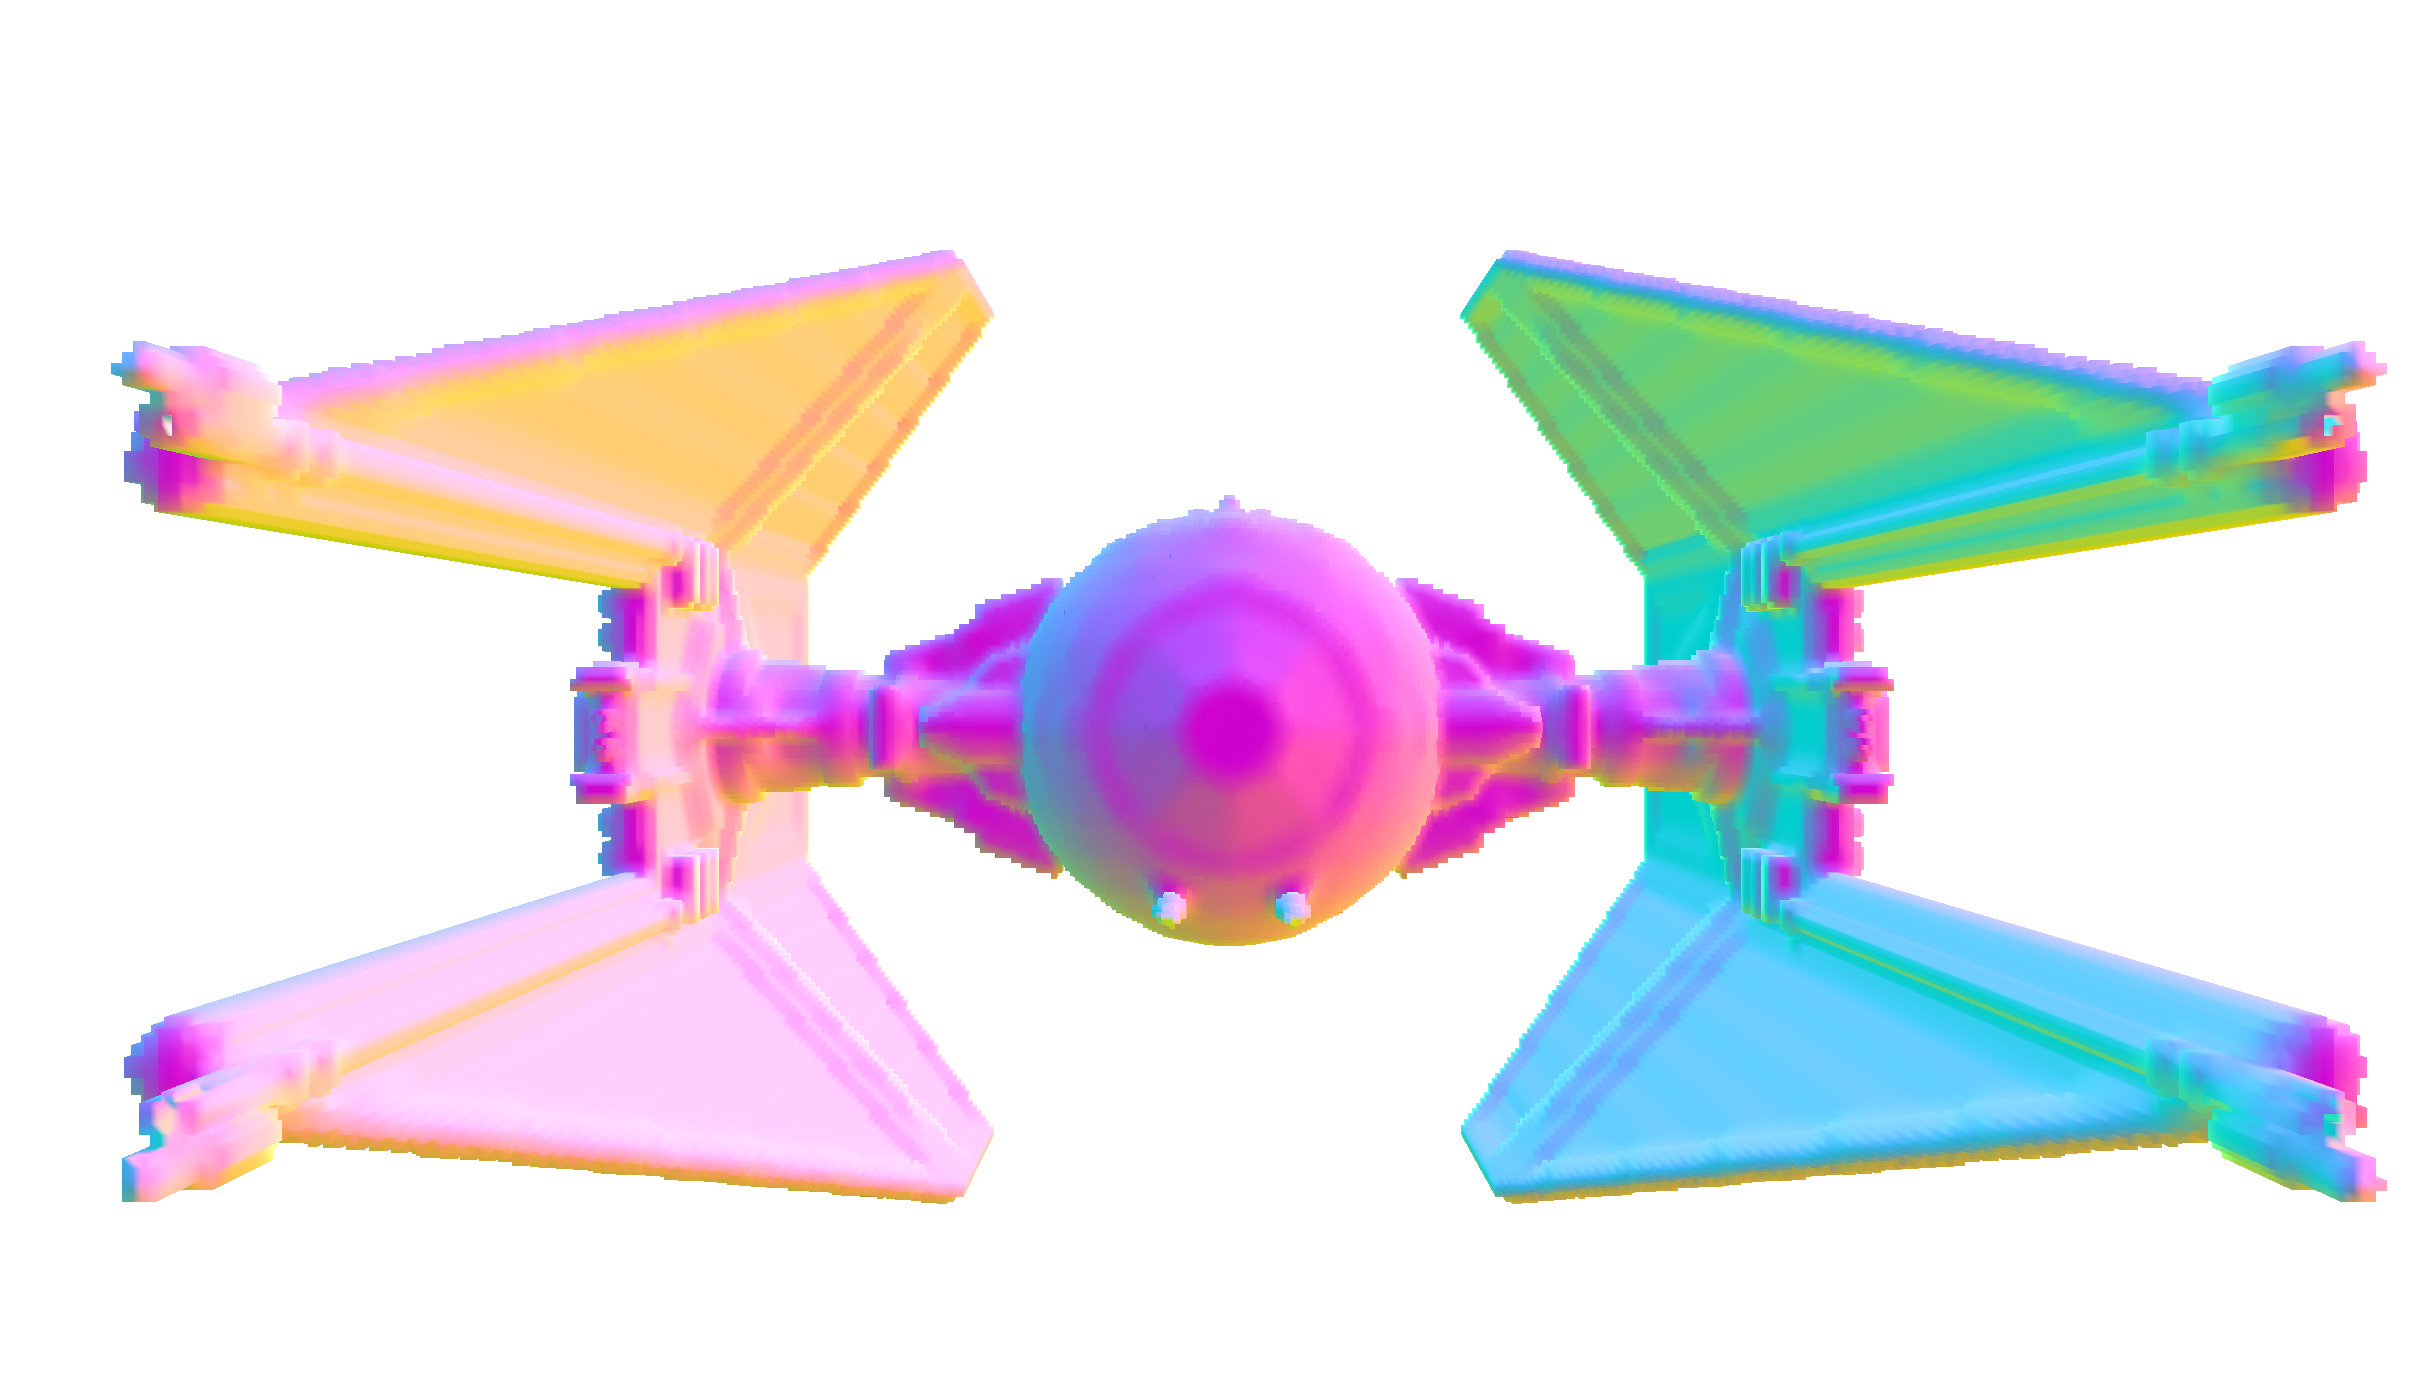
\includegraphics[width=0.43\textwidth]{pictures/tie256-VN-flat} \\
            %% 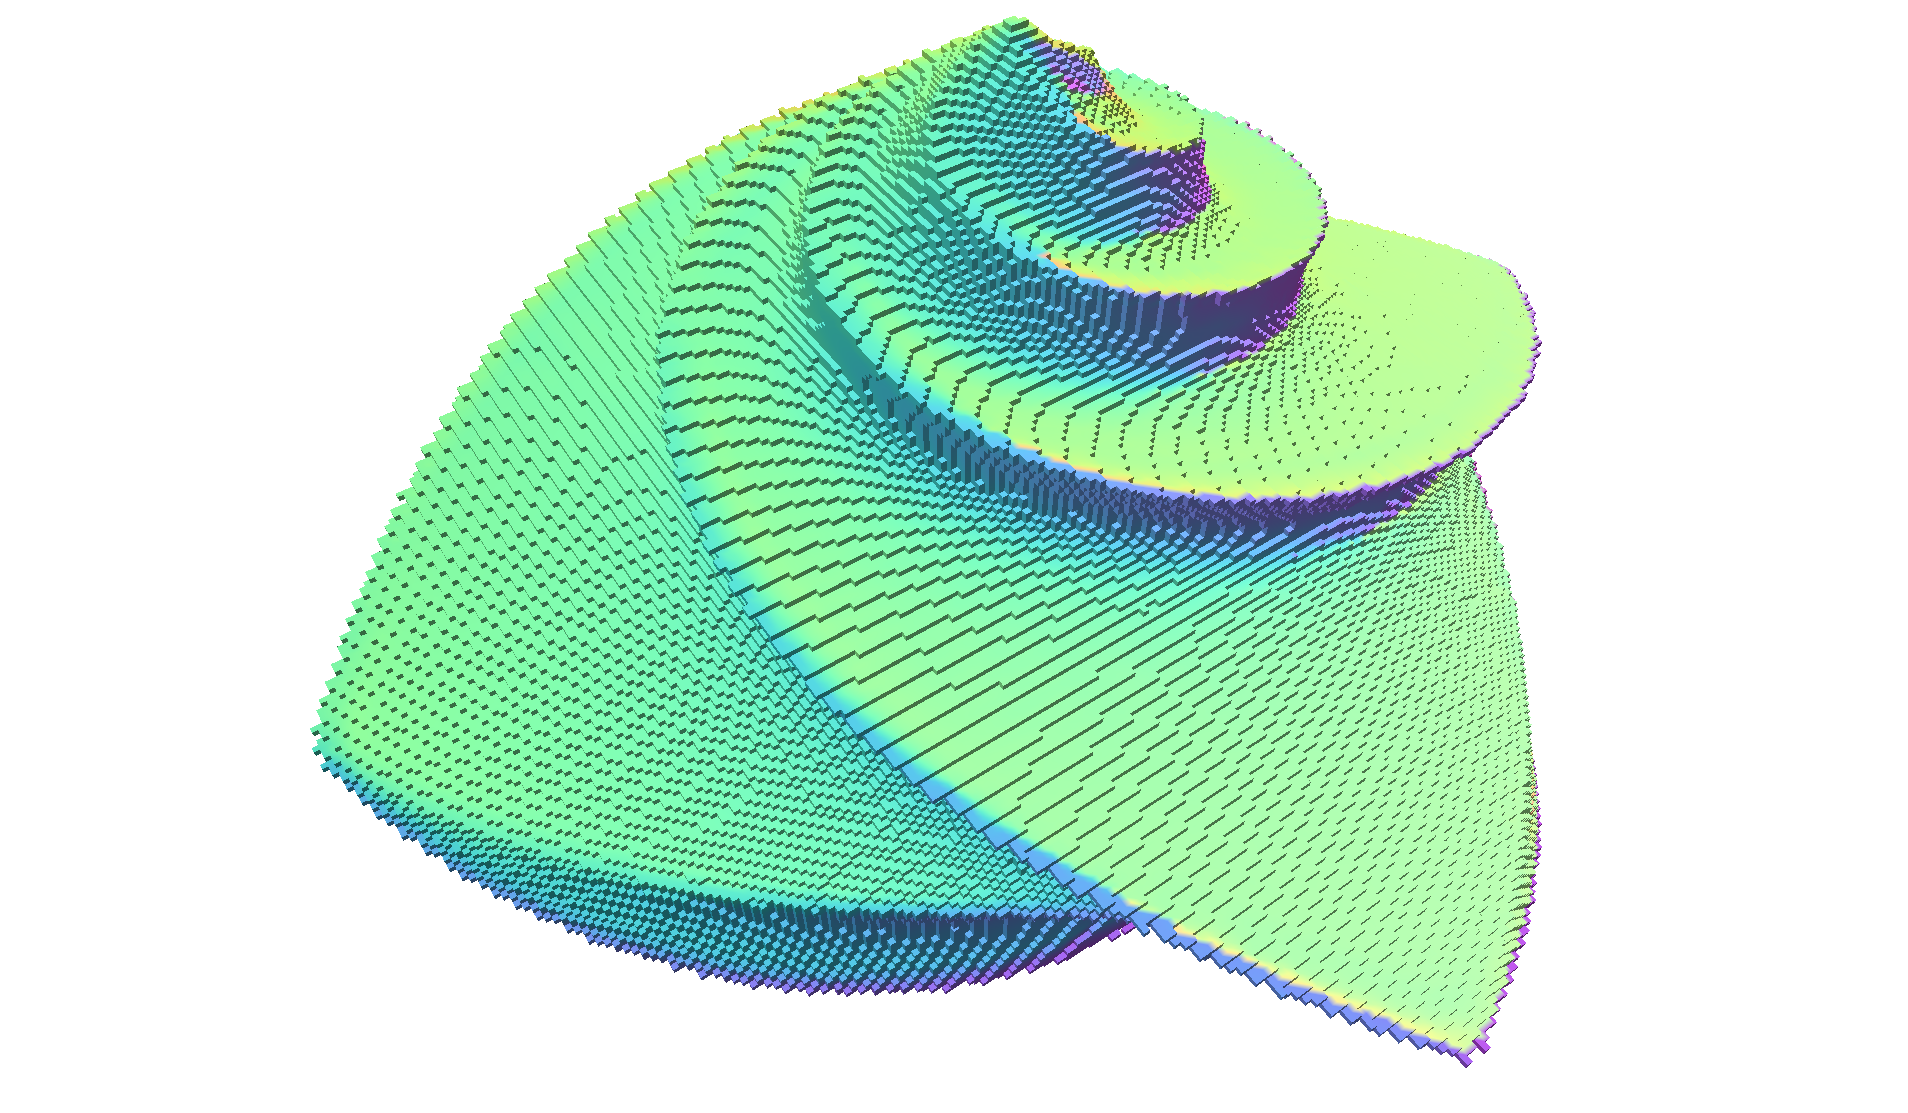
\includegraphics[width=0.4\textwidth]{pictures/octaflower-normal-estimation-cubes-NV} &
            %% 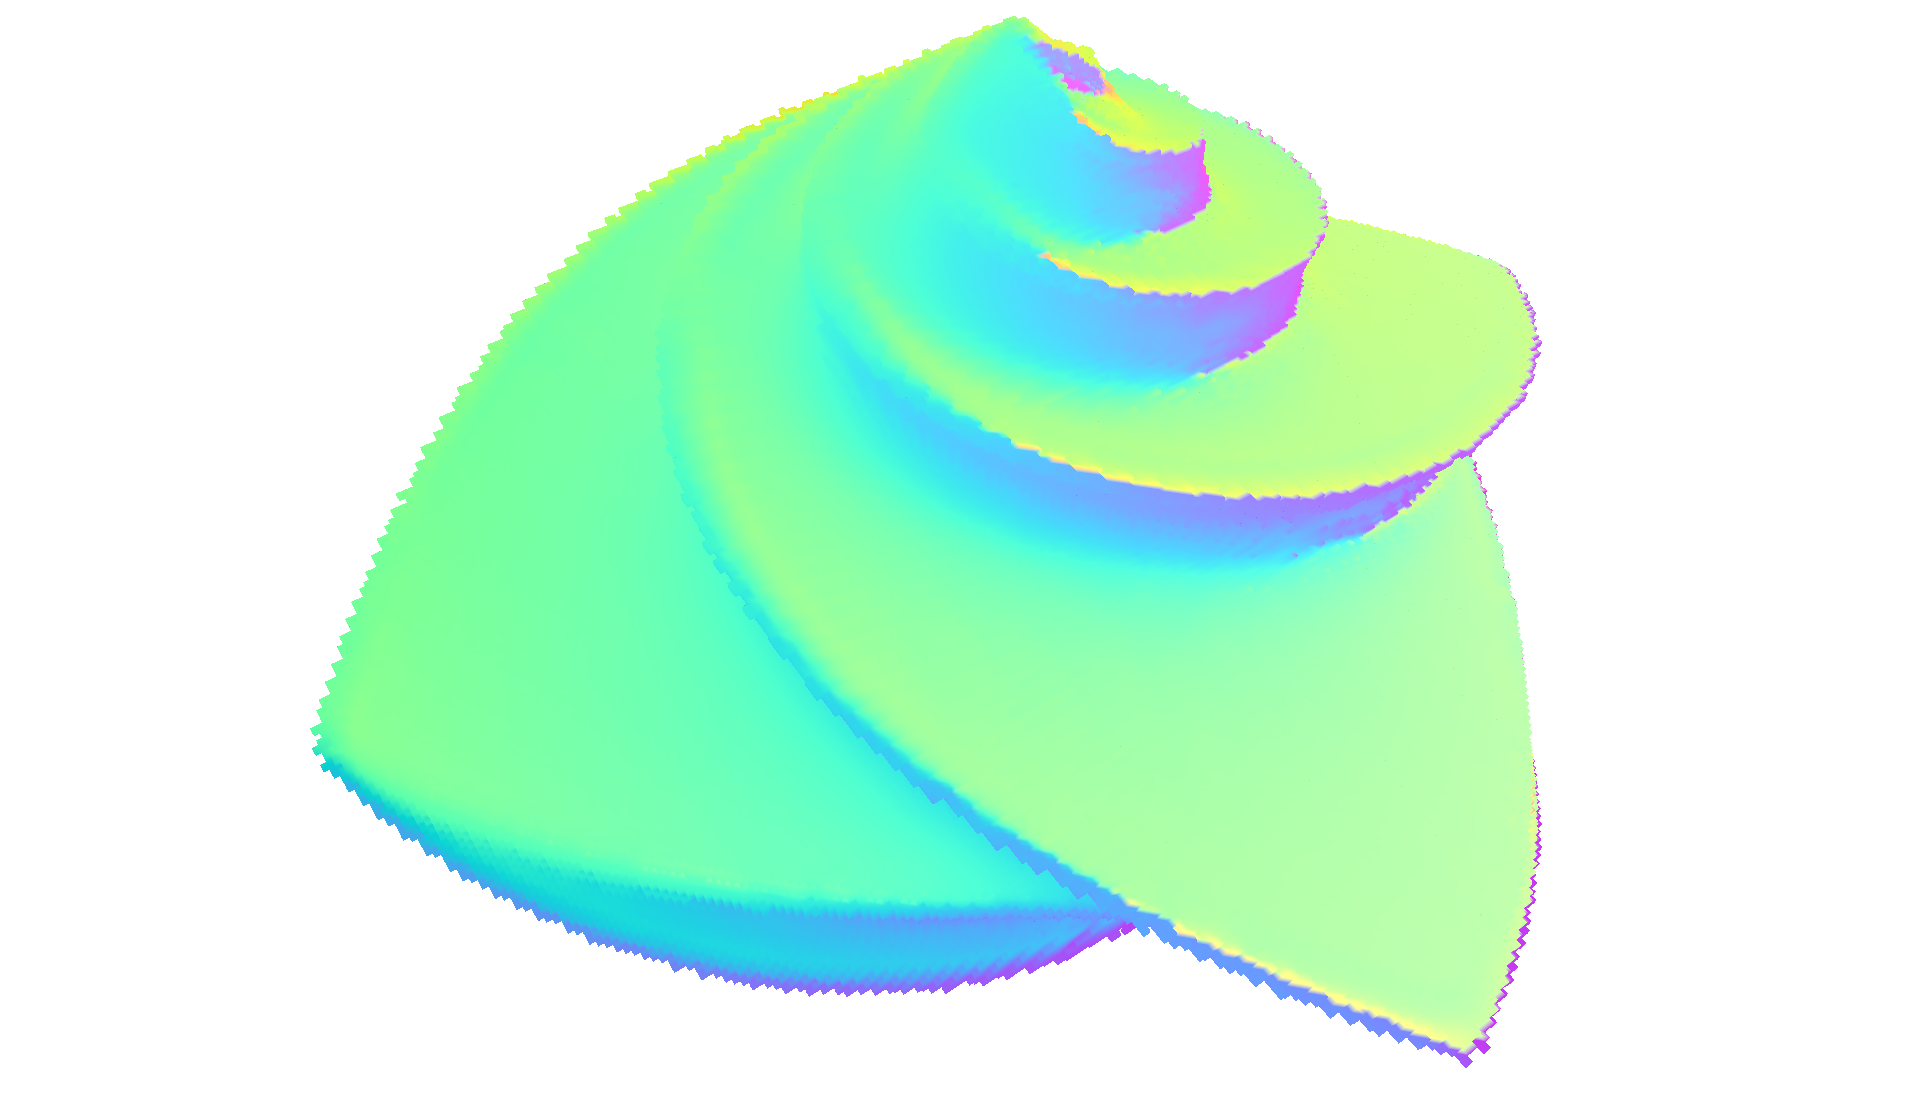
\includegraphics[width=0.4\textwidth]{pictures/octaflower-normal-estimation-smooth-NV} \\
            \hline
        \end{tabular}
        \caption{Examples of normals computed on a chinese dragon, then on an
        octaflower as a color map. First set displays II normals, second set
        uses the visibility algorithm to compute them. The normals are colored
        according to their orientation as $0.5 \cdot (n_i + \mathbbm{1})$. The
        right images are the smooth version of the left images. ``Integral
        Invariant normals'' are computed using a radius of $r=4.5$, while
        our normal estimator are computed using a deviation of $\sigma=4$, and so
        a radius of $r=2\sigma=8$}
        \label{fig:normals-estimation}
    \end{figure}

    %% Then, to compute the curvatures, we use the Corrected Normal Current
    %% estimator~\cite{lachaud:2022-dcg} which are based on the normals computed
    %% above.

    \paragraph{Application to curvature estimation.}
    In order to illustrate better that the visibility normals better
    take into account the sharp features of a digital surface while
    staying meaningfull in digitization of smooth parts, we compare
    the curvature estimates induced by different discrete normal
    estimators. We exploit the \emph{Corrected Normal Current (CNC)
        estimator}, whose theory is detailed in~\cite{lachaud:2022-dcg}
    and which can estimate all kinds of curvatures given positions and
    normals. It produces state-of-the-art curvature estimates on
    polygonal surfaces~\cite{lachaud:2020-cgf}, point clouds~\cite{lachaud:2023-cgf}, and even outperforms Integral Invariant
    curvature estimates~\cite{coeurjolly:2014-cviu} on digital
    surfaces~\cite{lachaud:2022-dcg}. Its implementation is also
    available in    \href{https://dgtal-team.github.io/doc-nightly/moduleCurvatureMeasures.html}{\textsc{DGtal}}.

    Figure~\ref{fig:fig-curvatures} displays the results of CNC curvature
    estimations on the digitization of a piecewise smooth shape
    ``Talking D20'', taken from
    \href{https://ten-thousand-models.appspot.com/detail.html?file_id=1533028}{Thingi10K}.
    We compare the differences obtained by just changing the discrete
    normal estimator (available in the \textsc{DGtal} library):
    (column II normals) Integral Invariant normals with $r=6$, (column
    CTriv normals) convolved trivial normals with $r=6$, (column
    Visibility normals) our proposed estimator (VN) with $\sigma=4$ and
    maximal visibility distance $2\sigma$. These parameters were
    chosen so that the respective computation windows of the different
    estimators are approximately the same.

    II estimator is good along digitization of smooth or flat parts of
    the dice, but presents curious artefacts near sharp features
    induced by the hollowed out numbers: this is due to the nature of
    II normal estimates, which computes a PCA of a ball centered on
    the point of interest and may include points on the other side of
    the saliencies.

    CTriv estimator only performs averaging of trivial normal
    directions along the surface. It behaves much better than II near
    features (although it tends to smooth curvatures) since it does
    not use information from across the gap. However some oscillations
    of the curvatures are distinguishable especially along the flat
    parts, and some curvature estimates are erroneous on smoother
    parts (like the edge above 6 for $\kappa_2$ or several dice
    vertices).

    VN estimator takes the best of the two previous approaches. It
    remains precise and stable on smooth and flat regions, while
    perfectly delineating sharp features and holes, whatever the kind
    of estimated curvatures. Its only drawback is the computation
    time, which is [TO COMPLETE], compared to $2.3$s for II and $0.1s$
    for CTriv.


    \newcommand{\MyZoom}[1]{%
        \begin{tikzpicture}[spy using outlines={circle,magnification=1.8,size=2cm,connect spies}]
        \node[inner sep=0pt] {\pgfimage[width=0.3\textwidth]{#1}};
        \spy[overlay,blue] on (0.4,0.2) in node at (-0.8,0.8);
        \end{tikzpicture}}
    % \newcommand{\MyZoom}[1]{\includegraphics[width=0.3\textwidth]{#1}}

    \begin{figure}
        \begin{center}
            \begin{tabular}{|c||c|c|c|}
                \hline
                Curv. & II normals & CTriv normals & Our normals \\ \hline \hline
                \raisebox{18mm}{$\kappa_1$} &
                \MyZoom{pictures/d20-k1-II.jpg} &
                \MyZoom{pictures/d20-k1-CTriv.jpg}&
                \MyZoom{pictures/d20-k1-VN.jpg}\\ \hline
                \raisebox{18mm}{$\kappa_2$} &
                \MyZoom{pictures/d20-k2-II.jpg} &
                \MyZoom{pictures/d20-k2-CTriv.jpg}&
                \MyZoom{pictures/d20-k2-VN.jpg}\\ \hline
                \raisebox{18mm}{$H$} &
                \MyZoom{pictures/d20-H-II.jpg} &
                \MyZoom{pictures/d20-H-CTriv.jpg}&
                \MyZoom{pictures/d20-H-VN.jpg}\\ \hline
                \raisebox{18mm}{$G$} &
                \MyZoom{pictures/d20-G-II.jpg} &
                \MyZoom{pictures/d20-G-CTriv.jpg}&
                \MyZoom{pictures/d20-G-VN.jpg}\\ \hline
            \end{tabular}
        \end{center}
        \caption{\label{fig:fig-curvatures}Estimation of curvatures using
          Corrected Normal Current estimators \cite{lachaud:2022-dcg}
          with a measure of radius $2$ for the shape ``Dice-20'' of
          Thingi10K database at resolution $256^3$. This estimator is
          parameterized by an input normal estimator: first column by
          ``Integral Invariant normals'' (radius $r=6$), second column
          by ``Convolved Trivial normals'' (radius $k=6$), third
          column by our presented normal estimator (deviation
          $\sigma=4$, radius $r=2\sigma=8$). Per row are displayed the
          estimated curvatures in order: first and second principal
          curvatures $\kappa_1$ and $\kappa_2$, mean curvature $H$,
          Gaussian curvature $G$. The range of curvature between deep
          blue and deep red is $\lbrack -0.1, 0.1 \rbrack$ with white
          color equal to $0$.}
    \end{figure}

%%%%%%%%%%%%%%%%%%%%%%%%%%%%%%%%%%%%%%%%%%%%%%%%%%%%%%%%%%%%%%%%%%%%%%


    \section{Conclusion}


%%%%%%%%%%%%%%%%%%%%%%%%%%%%%%%%%%%%%%%%%%%%%%%%%%%%%%%%%%%%%%%%%%%%%%
    \begin{credits}
        \subsubsection{\ackname}
        This work is partially supported by the French National Research Agency
        within the StableProxies project (ANR-22-CE46-0006).
%% \subsubsection{\discintname}
%% It is now necessary to declare any competing interests or to specifically
%% state that the authors have no competing interests. Please place the
%% statement with a bold run-in heading in small font size beneath the
%% (optional) acknowledgments\footnote{If EquinOCS, our proceedings submission
%% system, is used, then the disclaimer can be provided directly in the system.},
%% for example: The authors have no competing interests to declare that are
%% relevant to the content of this article. Or: Author A has received research
%% grants from Company W. Author B has received a speaker honorarium from
%% Company X and owns stock in Company Y. Author C is a member of committee Z.
    \end{credits}
%
% ---- Bibliography ----
%
% BibTeX users should specify bibliography style 'splncs04'.
% References will then be sorted and formatted in the correct style.
%
    \bibliographystyle{splncs04}
    \bibliography{biblio}

\end{document}
